\chapter{Eksperimen dan Analisis}
\label{chap:eksperimen}

Bab ini memaparkan eksperimen untuk memvalidasi tiga jalur yang dirancang pada Bab~\ref{chap:deskripsi-sistem}, yaitu preprocessing sinyal ECG secara \textit{real-time} di mikrokontroler, inferensi model CNN INT8 di ESP32-S3, dan \textit{pipeline edge-to-cloud} yang tahan terhadap putusnya koneksi. Eksperimen mencakup evaluasi model pada DS2 dan data lintas basis data, kuantisasi INT8, kesetaraan keluaran kode C terhadap Python, kinerja model di perangkat, akuisisi sinyal tubuh, serta pengukuran \textit{pipeline} MQTT dengan sumber sinyal \textit{replay} yang mencakup \textit{streaming} normal dan putusnya koneksi ke \textit{broker}. Pembahasan mencakup parameter eksperimen, karakteristik data, tempat dan waktu ujicoba, spesifikasi peralatan, hasil eksperimen per jalur, dan analisis yang dikaitkan kembali dengan tujuan pada Subbab~\ref{sec:tujuan}.

\section{Parameter Eksperimen}
\label{sec:parameter-eksperimen}

Parameter eksperimen dikelompokkan ke dalam tujuh kategori yang mengikuti tiga jalur pada tujuan penelitian. Target setiap metrik diambil dari rencana pengujian pada Tabel~\ref{tab:pengujian-model} dan Tabel~\ref{tab:pengujian-pipeline} serta uraian pengujian \textit{pipeline}, sehingga hasil pada bab ini dapat dinilai langsung terhadap rencana tersebut. Kategori, metrik, target, dan alasan pemilihannya dirangkum pada Tabel~\ref{tab:parameter-eksperimen}.

\begin{center}
  \setstretch{1.0}
  \setlength{\tabcolsep}{4pt}
  \renewcommand{\arraystretch}{1.15}
  \small
  \begin{longtable}{|>{\RaggedRight\arraybackslash}p{2.5cm}|>{\RaggedRight\arraybackslash}p{3.4cm}|>{\RaggedRight\arraybackslash}p{3.4cm}|>{\RaggedRight\arraybackslash}p{3.5cm}|}
    \caption{Parameter eksperimen per kategori}
    \label{tab:parameter-eksperimen} \\
    \hline
    \rowcolor{headgray}
    \textbf{Kategori} & \textbf{Metrik} & \textbf{Target} & \textbf{Alasan dan Acuan} \\
    \hline
    \endfirsthead
    \hline
    \rowcolor{headgray}
    \textbf{Kategori} & \textbf{Metrik} & \textbf{Target} & \textbf{Alasan dan Acuan} \\
    \hline
    \endhead
    \hline
    \endfoot
    a. Kualitas klasifikasi &
    \textit{Recall}, \textit{precision}, F1-\textit{score}, \textit{specificity}, AUC, dan \textit{confusion matrix} pada DS2, \textit{recall} per kelas AAMI dan per pasien, serta F1 dan \textit{recall} kelas S pada data uji SVDB dan INCART &
    Dilaporkan pada \textit{threshold} hasil kalibrasi data validasi (F1 maksimum). Lintas basis data dilaporkan sebagai pembanding ablasi (Tabel~\ref{tab:pengujian-model}) &
    Pembagian \textit{inter-patient} dan pengelompokan kelas AAMI mengikuti de Chazal~\cite{dechazal_2004} agar sebanding dengan literatur. \textit{Accuracy} dihitung tetapi tidak dijadikan acuan \\
    \hline
    b. Dampak kuantisasi &
    Selisih (\textit{delta}) tiap metrik antara \textit{float32} dan INT8 pada DS2 yang identik &
    $|\Delta \textit{recall}| < 0{,}02$ (Tabel~\ref{tab:pengujian-model}) &
    Ambang ini juga diperiksa otomatis oleh skrip daftar periksa \textit{proof of concept} sehingga dampak kuantisasi diukur, bukan diasumsikan \\
    % sumber: laporan/buku-pa/bab/bab3.tex tab:pengujian-model; model/scripts/check_poc.py tabel_delta() (abs(d_recall) < 0.02)
    \hline
    c. Kinerja di perangkat &
    Latensi inferensi per detak, \textit{tensor arena}, \textit{heap} bebas, pemakaian RAM dan \textit{flash}, serta ukuran model INT8 &
    Latensi lebih kecil dari interval antardetak, muat di SRAM perangkat, dan ukuran model $<$ 25 KB (Tabel~\ref{tab:pengujian-model}) &
    Inferensi harus selesai sebelum detak berikutnya agar \textit{real-time}. Batas 25 KB adalah disiplin rancangan, bukan kapasitas, karena \textit{flash} berukuran 16 MB \\
    % sumber: model/config.py (MAX_MODEL_KB = 25 dan komentarnya); firmware/platformio.ini (ESP32-S3 N16R8, 16MB flash, 8MB PSRAM)
    \hline
    d. Preprocessing di mikrokontroler &
    Selisih keluaran kode C terhadap Python, beban komputasi per sampel, puncak beban, dan jumlah sampel hilang &
    Label akhir identik pada setiap detak acuan, selisih probabilitas $\leq$ 0,02, serta selisih filter dan \textit{z-score} $\leq 10^{-3}$ (Tabel~\ref{tab:pengujian-model}), dan tanpa sampel hilang (Subbab~\ref{subsec:preprocessing-ecg}) &
    Data acuan keluaran Python memastikan C dan Python menghitung hal yang sama. Sampel yang hilang merusak interval R-R yang menjadi masukan cabang ritme \\
    % sumber: laporan/buku-pa/bab/bab3.tex Subbab Akuisisi Sinyal ECG (antrean ISR, sampel tidak hilang); firmware/test/golden_ref.h
    \hline
    e. Akuisisi sinyal tubuh &
    Ayunan sinyal ADC (\textit{count} dan mV), persentase dengung jala-jala 50 Hz, jumlah R-\textit{peak} terdeteksi, dan proporsi BPM dalam rentang wajar &
    Ayunan tersaring mencapai ambang 60 \textit{count}
, interval R-R 300--1500 ms dengan $|\Delta \mathrm{RR}| \leq 200$ ms selama 30 detik (Subbab~\ref{subsec:pipeline-edge-cloud}) &
    \textit{Flag lead-off} AD8232 tidak menjamin adanya sinyal, sehingga ayunan ADC absolut dijadikan acuan \\
    % sumber: laporan/buku-pa/bab/bab3.tex gerbang kualitas (AMBANG_AYUN 60, RR 300-1500 ms, |dRR| <= 200 ms, 30 detik); model/CLAUDE.md Jebakan "Telemetri akuisisi bisa berbohong" butir (1)
    \hline
    f. \textit{Pipeline edge-to-cloud} &
    PDSR, latensi \textit{end-to-end} (median dan p95), jumlah entri \textit{ring buffer}, data hilang, waktu \textit{flush}, dan paket ganda &
    PDSR $\geq$ 95\%, latensi $\leq$ 2 detik, tidak \textit{overflow} dalam $\pm$27.000 rekaman, tanpa kehilangan data, \textit{flush} $\leq$ 60 detik, dan duplikat QoS 1 dikenali (Tabel~\ref{tab:pengujian-pipeline}) &
    Bufer lokal di sisi \textit{edge} mempertahankan kontinuitas data ketika koneksi putus~\cite{resilient_edge_cloud}, sedangkan detak yang hilang bertepatan dengan kejadian aritmia tidak dapat direkonstruksi di sisi \textit{cloud}. Target latensi dinilai pada median, sesuai pencatatan latensi rata-rata pada rencana pengujian, sedangkan p95 dilaporkan agar ekor sebarannya ikut terlihat \\
    % sumber: laporan/buku-pa/bab/bab3.tex tab:pengujian-pipeline
    \hline
    g. Konsumsi daya &
    Arus dan daya rata-rata (mA dan mW) &
    Dilaporkan per mode operasi (Tabel~\ref{tab:pengujian-model}) &
    Konsumsi daya diukur sebagai acuan awal dan tidak dioptimasi (Subbab~\ref{sec:batasan-masalah}) \\
    \hline
  \end{longtable}
\end{center}

Berdasarkan Tabel~\ref{tab:parameter-eksperimen}, kategori b sampai f memiliki target yang dapat diverifikasi secara langsung, baik berupa ambang angka maupun syarat lulus seperti label akhir yang identik pada setiap detak acuan. Kategori a dan g tidak memiliki ambang angka pada rencana pengujian. Kualitas klasifikasi karena itu dilaporkan pada titik operasi hasil kalibrasi data validasi dan dibandingkan dengan penelitian terkait yang memakai protokol \textit{inter-patient} pada analisis hasil, sedangkan konsumsi daya dilaporkan sebagai acuan awal. \textit{Accuracy} tetap dihitung tetapi tidak dijadikan acuan, karena 89,0\% detak DS2 berlabel Normal sehingga menebak Normal untuk seluruh detak sudah menghasilkan \textit{accuracy} sekitar 0,89.
% sumber: model/data/processed/test.npz (49.656 detak, y.mean() = 0,1098, Normal 89,02%); model/CLAUDE.md decision "Metrik yang dipantau" (accuracy tidak dipakai)

\section{Karakteristik Data}
\label{sec:karakteristik-data}

Karakteristik data diuraikan dalam lima butir, yaitu data sekunder untuk pelatihan dan pengujian model, data primer hasil rekaman perangkat, sumber sinyal \textit{replay}, penyelarasan pemrosesan antara komputer dan perangkat, serta data telemetri yang dikirim ke \textit{cloud}.

\subsubsection{Data Sekunder untuk Pelatihan dan Pengujian}

Data sekunder utama adalah MIT-BIH \textit{Arrhythmia Database} yang terdiri atas 48 rekaman dengan frekuensi sampel 360 Hz pada sadapan MLII~\cite{moody_mark_2001}. Rekaman 102 dan 104 dikeluarkan karena tidak memiliki kanal MLII, sedangkan rekaman 107 dan 217 dikeluarkan karena berisi detak alat pacu jantung, sehingga tersisa 44 rekaman. Label anotasi dipetakan ke kelas biner Normal dan Aritmia sesuai Tabel~\ref{tab:pemetaan-label}. Rekaman dibagi menjadi DS1 dan DS2 mengikuti pembagian \textit{inter-patient} de Chazal~\cite{dechazal_2004}, dan lima rekaman DS1, yaitu 101, 114, 201, 220, dan 223, dipisahkan sebagai data validasi (VAL).
% sumber: model/config.py (FS = 360, PACED_EXCLUDED = [102, 104, 107, 217], VAL_RECORDS = [101, 114, 201, 220, 223], DS2 22 rekaman); model/CLAUDE.md Fase 0 (48 record)

Setiap rekaman DS1 ditumpuk menjadi tiga salinan, yaitu satu salinan bersih dan dua salinan yang posisi segmentasinya digeser dengan \textit{jitter} empiris. Besar pergeserannya diambil ulang dari sebaran \textit{error} detektor R-\textit{peak} yang diukur sendiri, mengadaptasi gagasan augmentasi \textit{jitter}~\cite{dias_2021}. DS2 tidak diberi \textit{jitter} sehingga mewakili anotasi tanpa \textit{error} segmentasi. DS2 dipakai sebagai ukuran pada ablasi yang menentukan ukuran \textit{window} dan jumlah salinan \textit{jitter}, sedangkan pemilihan \textit{epoch} dan \textit{threshold} hanya memakai VAL, sehingga angka DS2 pada bab ini bukan data uji yang sepenuhnya belum tersentuh untuk dua keputusan pertama. Selain MIT-BIH, rekaman SVDB (128 Hz) dan INCART (257 Hz) di-\textit{resample} ke 360 Hz, lalu setiap rekaman keempat dalam urutan tersortir disisihkan sebagai data uji \textit{held-out}, yang selanjutnya disebut data uji SVDB dan data uji INCART. Sisa rekaman SVDB dan INCART hanya dipakai melatih varian ablasi, bukan model yang dikuantisasi. Komposisi seluruh himpunan data ditunjukkan pada Tabel~\ref{tab:dataset}.
% sumber: model/config.py (JITTER_MODEL = "empiris", JITTER_SALINAN = 2, SPLIT_SETIAP_KE = 4, DATASETS svdb fs 128 dan incartdb fs 257, komentar Fase A/B DB_LATIH); model/CLAUDE.md decision "Augmentasi jitter", "Model jitter", "Database LATIH" (mitdb saja, mitdb+svdb dipakai HANYA di ablasi) dan "Validation set"; model/artifacts/metrics/ablasi/lintas_db.csv (varian ablasi dievaluasi pada TEST-B dan TEST-C)

\begin{table}[!ht]
  \centering
  \caption{Komposisi himpunan data sekunder}
  \label{tab:dataset}
  \setstretch{1.0}
  \setlength{\tabcolsep}{4pt}
  \renewcommand{\arraystretch}{1.15}
  \small
  \begin{tabular}{|>{\RaggedRight\arraybackslash}p{1.9cm}|>{\RaggedRight\arraybackslash}p{2.9cm}|>{\RaggedRight\arraybackslash}p{3.2cm}|>{\centering\arraybackslash}p{1.5cm}|>{\RaggedRight\arraybackslash}p{3.0cm}|}
    \hline
    \rowcolor{headgray}
    \textbf{Himpunan} & \textbf{Sumber} & \textbf{Jumlah Data} & \textbf{Aritmia (\%)} & \textbf{Kegunaan} \\
    \hline
    DS1 latih & 17 rekaman MIT-BIH & 121.857 baris (40.619 detak $\times$ 3 salinan) & 10,1 & Pelatihan model \\
    \hline
    VAL & 5 rekaman MIT-BIH (bagian DS1) & 31.047 baris (10.349 detak $\times$ 3 salinan) & 10,1 & Pemilihan \textit{epoch} dan kalibrasi \textit{threshold} \\
    \hline
    DS2 & 22 rekaman MIT-BIH & 49.656 detak & 11,0 & Pengujian utama \\
    \hline
    Uji SVDB & 20 rekaman SVDB & 44.704 detak & 15,9 & Uji lintas basis data \\
    \hline
    Uji INCART & 19 rekaman INCART & 41.108 detak & 12,6 & Uji lintas basis data \\
    \hline
  \end{tabular}
\end{table}
% sumber: numpy atas model/data/processed/train.npz (152.904 baris, 22 rekaman, 50.968 detak x 3; VAL 31.047 baris = 10.349 x 3; latih 121.857 = 40.619 x 3; aritmia 10,11%), test.npz (49.656, 22 rekaman, 10,98%), test_svdb.npz (44.704, 20 rekaman, 15,88%), test_incartdb.npz (41.108, 19 rekaman, 12,57%)

Berdasarkan Tabel~\ref{tab:dataset}, DS1 secara keseluruhan memuat 22 rekaman dengan 152.904 baris setelah augmentasi, dan proporsi aritmia pada DS1 maupun DS2 berada di kisaran 10--11\%. Ketidakseimbangan kelas ini menjadi alasan \textit{class weight} dipakai saat pelatihan dan \textit{accuracy} tidak dijadikan acuan. Data uji SVDB dan INCART bersama-sama memuat 85.812 detak dari 39 rekaman \textit{held-out} dengan proporsi aritmia yang lebih tinggi, sehingga keduanya menguji generalisasi terhadap kondisi akuisisi dan sebaran kelas yang berbeda dari MIT-BIH.
% sumber: model/data/processed/train.npz (152.904 baris); model/CLAUDE.md decision "Strategi imbalance" (class_weight balanced) dan "Database LATIH" (85.812 beat, 39 pasien); 44.704 + 41.108 = 85.812

\subsubsection{Data Primer dari Perangkat}

Data primer berupa rekaman sinyal mentah dari modul AD8232 yang dicuplik ADC ESP32-S3 pada 360 Hz dan disimpan sebagai berkas CSV berisi nilai \textit{count} ADC 12-bit, dengan alur perekaman pada Subbab~\ref{subsec:antarmuka-perangkat}. Rekaman yang sempat dijeda terdiri atas beberapa segmen, dan durasinya dihitung dari jumlah sampel seluruh segmen tanpa waktu jeda. Rekaman yang diambil selama pengembangan hanya dipakai untuk menyusun prosedur perekaman dan menguji alat analisis, sehingga tidak dilaporkan sebagai hasil. Data primer yang dilaporkan berasal dari pengujian rekaman resmi, yaitu sebanyak \PlaceholderData{jumlah rekaman} rekaman yang diambil pada \PlaceholderData{tanggal sesi perekaman} dengan durasi \PlaceholderData{durasi terpendek sampai terpanjang} detik per rekaman, atau total sekitar \PlaceholderData{total durasi} detik. Rekaman berasal dari \PlaceholderData{jumlah dan kode subjek} subjek sehat dengan konfigurasi Lead II dan elektroda \textit{wet-gel}. Identitas subjek dianonimkan dan pengambilan data bukan uji klinis, sesuai Batasan Masalah pada Subbab~\ref{sec:batasan-masalah}.
% PLACEHOLDER-DATA data-primer: jumlah rekaman resmi, tanggal sesi, durasi terpendek-terpanjang dan total (detik), jumlah dan kode subjek, beserta konfirmasi persetujuan subjek. Prosedur: model/docs/akuisisi-walkthrough.md §3-§5 (rekam dengan B3: pendek mulai/jeda/lanjut, tahan simpan; make pull -> model/data/recordings/<tanggal-jam>.csv). Hitung: ls model/data/recordings/*.csv | wc -l (hanya rekaman resmi, mulai 13 Okt 2026); durasi = n pada header "# fs=360 n=..." dibagi 360
% sumber: rekaman uji coba 10 Sep - 11 Okt 2026 (27 berkas) diarsipkan di model/data/arsip/rekaman-uji-coba/README.md dan tidak dipakai sebagai hasil; laporan/buku-pa/bab/bab1.tex Batasan Masalah butir 3 dan 4

Penempatan elektroda mengikuti konfigurasi Lead II sebagaimana ditunjukkan pada Gambar~\ref{fig:4-elektroda}.

% PLACEHOLDER-GAMBAR fig:4-elektroda  (foto user, bukan Claude)
% Jenis      : foto dokumentasi, portrait
% Pesan      : letak tiga elektroda wet-gel untuk Lead II
% Elemen     : torso dari bahu sampai pinggang TANPA wajah, tato, atau penanda identitas; RA di bawah selangka kanan; LA di bawah rusuk kiri; RL di bawah rusuk kanan sebagai referensi
% Alur baca  : atas ke bawah, RA, lalu LA, lalu RL
% Teks       : label persis "RA", "LA", "RL"
% Bahan repo : model/docs/akuisisi-walkthrough.md §1
% Ukuran     : height=0.4\textheight,keepaspectratio
\begin{figure}[!ht]
  \centering
  \PlaceholderGambar{Foto dokumentasi}{posisi elektroda RA, LA, dan RL pada torso subjek tanpa wajah}
  \caption{Posisi elektroda Lead II}
  \label{fig:4-elektroda}
\end{figure}

Pada Gambar~\ref{fig:4-elektroda}, sumbu dari RA ke LA meniru sadapan MLII yang dipakai MIT-BIH, sehingga morfologi QRS rekaman perangkat sebanding dengan data latih.
% sumber: model/docs/akuisisi-walkthrough.md §1 (RA bawah selangka kanan, LA bawah rusuk kiri, RL bawah rusuk kanan sebagai referensi; sumbu merah ke kuning meniru MLII)

Rekaman yang tidak memenuhi kriteria kualitas sinyal tetap disimpan karena menjadi bukti dalam mendiagnosis gangguan akuisisi. Kualitas setiap rekaman dinilai dari ayunan sinyal ADC absolut, kandungan dengung jala-jala, dan jumlah R-\textit{peak} terdeteksi, dan hasilnya dibahas pada Subbab~\ref{subsec:hasil-tujuan1}.
% sumber: model/CLAUDE.md Jebakan "Telemetri akuisisi bisa berbohong"; model/docs/akuisisi-walkthrough.md §6 dan §8

\subsubsection{Sumber Sinyal \textit{Replay}}

Untuk menguji jalur hilir secara deterministik tanpa bergantung pada elektroda, perangkat dilengkapi sumber sinyal \textit{replay} yang dipilih dari menu Sumber sinyal (Subbab~\ref{subsec:antarmuka-perangkat}). Sumber yang dipakai pada seluruh pengujian bab ini adalah sinyal mentah data acuan, yaitu 2.400 sampel pertama rekaman 208 dari DS1 atau sekitar 6,67 detik, yang dikonversi sekali menjadi nilai \textit{count} ADC saat \textit{setup}. Ketika \textit{replay} aktif, \textit{timer interrupt} menyalin nilai dari tabel tersebut sebagai pengganti pembacaan ADC, sedangkan filter, deteksi R-\textit{peak}, segmentasi, inferensi, dan pengiriman MQTT tidak berubah sama sekali. Karena hanya sumber sampel yang diganti, hasil pengukuran pada jalur hilir dapat dijadikan acuan untuk sinyal yang berasal dari ADC, dengan catatan syarat stabilisasi dan syarat R-R pada gerbang kalibrasi dilewati selama \textit{replay} dan laju detaknya sekitar 1,6 detak per detik. Sumber \textit{replay} rekaman tersimpan juga tersedia, tetapi tidak dipakai pada pengujian yang dilaporkan.
% sumber: firmware/test/golden_ref.h (record 208 DS1, GOLDEN_N 2400, golden_raw); 2400 / 360 = 6,67 detik; firmware/src/akuisisi.cpp on_timer() dan sim_counts (tabel replay acuan); model/docs/firmware-walkthrough.md §5c "Terukur di board" (11 beat per putaran 6,67 detik, 1,58 beat/detik)

Satu putaran sinyal \textit{replay} memuat 9 detak beranotasi, tetapi perangkat mengeluarkan 11 detak per putaran karena sambungan antarputaran menghasilkan dua detak tambahan. Perhitungan data hilang pada uji \textit{pipeline} memakai angka 11, karena yang dihitung adalah detak yang benar-benar dikirim perangkat. Rekaman 208 juga bersifat aritmik sehingga tidak dapat melewati gerbang R-R pada fase kalibrasi. Pada \textit{firmware} akhir, pelewatan gerbang tersebut melekat pada sumber \textit{replay} dan berhenti begitu sumber kembali ke sensor, sehingga tidak dapat terbawa ke perekaman sinyal tubuh.
% sumber: firmware/test/golden_ref.h (GOLDEN_N_BEAT 9); model/docs/firmware-walkthrough.md §5c "Terukur di board" (11 beat per putaran, akuntansi MQTT pakai 11); model/docs/mqtt-walkthrough.md §3.1b (replay record 208 aritmik, gerbang kalibrasi dilewati selama replay); firmware/src/gerbang.cpp gerbang_nilai_fase() (bypass replay)

\subsubsection{Penyelarasan Pemrosesan antara Komputer dan Perangkat}

Model hanya berlaku di perangkat apabila \textit{window} yang diterimanya identik dengan \textit{window} saat pelatihan. Filter Butterworth pada kedua sisi bersifat kausal dengan koefisien SOS yang sama, karena koefisien untuk kode C dihasilkan otomatis dari Python ke berkas \textit{header} C. Filter kausal menimbulkan \textit{group delay} sebesar 4 sampel, dan pergeseran ini tidak dikoreksi melainkan dipelajari model, sehingga puncak R berada di indeks 132 pada \textit{window} 256 sampel, yaitu 128 sampel sebelum R ditambah 4. Setiap \textit{window} dinormalisasi \textit{z-score} secara mandiri, dan model INT8 beserta \textit{threshold} 0,80 dibawa ke \textit{firmware} melalui berkas \textit{header} C yang juga dihasilkan otomatis.
% sumber: firmware/include/ecg_preproc.h (GENERATED oleh model/scripts/export_golden.py, ECG_WIN_PRE 128, ECG_WIN_POST 128, ECG_GROUP_DELAY 4); model/config.py (R_IN_WINDOW = WIN_PRE + 4); firmware/include/model_int8.h (GENERATED oleh export_model_h.py, ECG_THRESHOLD 0.8f); model/CLAUDE.md Jebakan "Group delay filter kausal"

Di perangkat, posisi R-\textit{peak} berasal dari detektor Pan-Tompkins, bukan dari anotasi. Keluaran detektor karena itu dikompensasi sebesar 38 sampel, dicari puncak sebenarnya dalam rentang $\pm$25 sampel, lalu dikurangi \textit{group delay} 4 sampel, sehingga puncak R mendarat di indeks yang sama dengan data latih. Kesetaraan seluruh rantai ini diuji dengan data acuan (\textit{golden reference}), yaitu keluaran setiap tahap Python pada rekaman 208 yang dibandingkan dengan keluaran kode C.

% sumber: firmware/include/ecg_preproc.h (ECG_PT_OFFSET 38, ECG_PT_REFINE 25, ECG_GROUP_DELAY 4); model/CLAUDE.md decision "Segmentasi on-device"; firmware/test/golden_ref.h

\subsubsection{Data Telemetri}

Data telemetri adalah hasil klasifikasi per detak yang dikirim perangkat ke ThingsBoard dengan struktur \textit{field} sesuai Tabel~\ref{tab:payload-json}. \textit{Field} ts berisi waktu kejadian detak yang dihitung dari posisi R-\textit{peak} dan jam sistem yang disinkronkan, bukan waktu kirim, sehingga detak yang tertahan di bufer tetap membawa waktu kejadiannya. Di dalam \textit{ring buffer} PSRAM, setiap detak disimpan sebagai struktur biner berukuran 40 byte dan baru disusun menjadi JSON saat dikirim. Pengukuran \textit{pipeline} memakai dua sumber data, yaitu telemetri yang dibaca dari REST API ThingsBoard untuk menghitung latensi dan pencacah paket pada \textit{firmware} yang dibaca melalui serial untuk menghitung PDSR.
% sumber: firmware/include/ecg_mqtt.h (ecg_mqtt_beat_t 40 byte, ts = ts_base_ms + beat.ms, PDSR dihitung per paket); dashboard/ukur_pipeline.py (docstring: latensi dari REST ThingsBoard, PDSR dari pencacah firmware lewat serial)

\section{Tempat Ujicoba}
\label{sec:tempat-ujicoba}

Seluruh uji dilakukan di lingkungan non-klinis sesuai Batasan Masalah. Perekaman sinyal tubuh dilakukan di \PlaceholderData{tempat perekaman} dengan subjek duduk diam dan perangkat dicatu \textit{powerbank}, sehingga tidak ada sambungan listrik ke jala-jala selama perekaman. Uji \textit{pipeline} dilakukan pada jaringan WiFi rumah, yaitu ESP32-S3 terhubung ke titik akses yang sama dengan komputer yang menjalankan ThingsBoard di dalam \textit{container} Docker, sehingga \textit{broker} MQTT berada di jaringan lokal, bukan di server publik. Lingkungan ini dipilih karena seluruh komponen \textit{pipeline} dapat dikendalikan sendiri, termasuk pembekuan \textit{broker} untuk meniru putusnya koneksi. Jaringan WiFi tersebut tidak terisolasi dari perangkat lain sehingga \textit{channel contention} tetap dapat terjadi.
% sumber: dashboard/docker-compose.yml (thingsboard/tb-postgres, port 1883 MQTT dan 8080 UI di komputer lokal); model/docs/mqtt-walkthrough.md §7 ("broker ThingsBoard CE di laptop pada jaringan WiFi rumah") dan §7c (kontensi kanal WiFi rumah); model/docs/akuisisi-walkthrough.md §1 dan §3 (powerbank, USB laptop dicabut, subjek duduk diam); laporan/buku-pa/bab/bab1.tex Batasan Masalah butir 4
% PLACEHOLDER-DATA tempat-perekaman: tempat pengujian rekaman sinyal tubuh resmi (laboratorium atau bukan, nama laboratorium bila ada), dicatat penulis saat sesi perekaman resmi

Pelatihan model, ablasi, kuantisasi, dan uji unit kode C yang tidak memerlukan perangkat keras dijalankan di komputer pribadi. Pemisahan ini dimungkinkan karena tahap tersebut hanya membutuhkan data sekunder dan daya komputasi, sedangkan uji yang melibatkan sinyal tubuh dan jaringan memerlukan perangkat keras. Komputer yang sama juga menjalankan ThingsBoard saat uji \textit{pipeline}.


\section{Waktu Ujicoba}
\label{sec:waktu-ujicoba}

Kegiatan eksperimen berlangsung sejak Agustus 2026. Rentang setiap kegiatan pada Tabel~\ref{tab:waktu-ujicoba} disusun dari catatan pengembangan, yaitu riwayat \textit{commit} repositori dan nama berkas rekaman, sehingga dapat berbeda beberapa hari dari tanggal percobaan yang sebenarnya.

\begin{table}[!ht]
  \centering
  \caption{Waktu pelaksanaan kegiatan eksperimen}
  \label{tab:waktu-ujicoba}
  \setstretch{1.0}
  \setlength{\tabcolsep}{4pt}
  \renewcommand{\arraystretch}{1.15}
  \small
  \begin{tabular}{|>{\RaggedRight\arraybackslash}p{8.2cm}|>{\RaggedRight\arraybackslash}p{4.4cm}|}
    \hline
    \rowcolor{headgray}
    \textbf{Kegiatan} & \textbf{Rentang Waktu} \\
    \hline
    Pengembangan model, yaitu penyiapan data, pelatihan, evaluasi, kuantisasi, dan ekspor & 24 Agustus -- 10 September 2026 \\
    % sumber: git log 3747551 (2026-08-24, scaffolding pipeline training) sampai ea78eb7 (2026-09-10, Fase 8)
    \hline
    \textit{Port} preprocessing ke kode C, inferensi di perangkat, alur hidup, dan \textit{firmware} utama & 10 -- 12 September 2026 \\
    % sumber: git log 8eaf44e (2026-09-10, golden reference) sampai 7698c58 (2026-09-12, firmware produksi)
    \hline
    Perekaman uji coba sinyal tubuh untuk menyusun prosedur akuisisi, pada rangkaian \textit{breadboard} dan rangkaian uji dengan peta pin PCB & 10 September -- 11 Oktober 2026 \\
    % sumber: model/data/arsip/rekaman-uji-coba/README.md (27 rekaman uji coba 20260910-1938.csv sampai 20261011-1834.csv, bukan hasil)
    \hline
    Biaya segmentasi di perangkat, ketahanan terhadap \textit{jitter}, dan penguncian \textit{window} & 12 -- 18 September 2026 \\
    % sumber: git log fce7cd1 (2026-09-12, Fase 6b) sampai cf5f5d5 (2026-09-18, retrain window 256)
    \hline
    Persiapan pengukuran daya dan sumber sinyal \textit{replay} & 16 -- 18 September 2026 \\
    % sumber: git log 50dc8d2 (2026-09-16, desain pengukuran daya) sampai 47ca6e6 (2026-09-18, replay golden_raw)
    \hline
    \textit{Dashboard} ThingsBoard dan \textit{pipeline} MQTT & 18 -- 19 September 2026 \\
    % sumber: git log b906903 (2026-09-18, dashboard) sampai 6fc426c (2026-09-19, perbaikan jam HW-6)
    \hline
    Ablasi lintas basis data, fitur, dan regime pelatihan & 19 September 2026 \\
    % sumber: git log 03c77f2 sampai 2acc531 (seluruhnya 2026-09-19)
    \hline
    Pengukuran ulang segmentasi di perangkat dengan model akhir & 13 Oktober 2026 \\
    % sumber: model/docs/segmentasi-deteksi-walkthrough.md §3 ("kondisi ukur: skrip yang sama, 13 Okt 2026")
    \hline
    \textit{Firmware} modular dengan antarmuka perangkat (layar, menu, perekaman berjeda), uji perangkat dan uji integrasi di papan, serta jalur pengukuran daya mandiri, pada rangkaian uji dengan peta pin PCB & 13 Oktober 2026 \\
    % sumber: git log 1fa4235 (2026-10-13, satu main.cpp pin map PCB, test perangkat), 9ba6498 (2026-10-13, main.cpp dipecah per modul), b012fa6 (2026-10-13, tangga ukur daya mandiri), 7476063 dan bca5773 (2026-10-13, menu), f6042b5 (2026-10-13, REC/JEDA di layar, rekam dengan jeda, board 29/29 dan native 23/23)
    \hline
    Pengujian rekaman sinyal tubuh resmi & \PlaceholderData{tanggal sesi} \\
    % PLACEHOLDER-DATA waktu-rekaman: tanggal setiap sesi pengujian rekaman resmi (mulai 13 Oktober 2026), dari nama berkas model/data/recordings/<tanggal-jam>.csv hasil make pull
    \hline
  \end{tabular}
\end{table}

Berdasarkan Tabel~\ref{tab:waktu-ujicoba}, pengembangan model mendahului pekerjaan perangkat keras, dan sebagian kegiatan berjalan beririsan karena hasil satu jalur langsung dipakai jalur lain. Hasil yang dilaporkan pada bab ini dikumpulkan sampai 13 Oktober 2026, kecuali hasil pengujian rekaman sinyal tubuh resmi yang dilaksanakan sesudah prosedur perekamannya ditetapkan pada tanggal tersebut. Pengujian \textit{pipeline} terverifikasi di perangkat pada 19 September 2026, dan segmentasi di perangkat diukur ulang dengan model akhir pada 13 Oktober 2026. Konsumsi daya tidak diukur dalam rentang tersebut, sebagaimana diuraikan pada Subbab~\ref{subsec:hasil-tujuan2}.
% sumber: git log 6fc426c (2026-09-19, perbaikan jam yang menuntaskan uji pipeline); model/data/recordings/README.md (rekaman resmi dimulai 13 Okt 2026); model/docs/segmentasi-deteksi-walkthrough.md §3 (13 Okt 2026)


\section{Spesifikasi Peralatan Ujicoba}
\label{sec:spesifikasi-peralatan}

Peralatan yang digunakan terdiri atas perangkat keras dan perangkat lunak. Spesifikasi perangkat keras beserta kegunaannya ditunjukkan pada Tabel~\ref{tab:perangkat-keras-uji}.

\begin{table}[!ht]
  \centering
  \caption{Spesifikasi perangkat keras ujicoba}
  \label{tab:perangkat-keras-uji}
  \setstretch{1.0}
  \setlength{\tabcolsep}{4pt}
  \renewcommand{\arraystretch}{1.15}
  \small
  \begin{tabular}{|>{\RaggedRight\arraybackslash}p{2.6cm}|>{\RaggedRight\arraybackslash}p{5.4cm}|>{\RaggedRight\arraybackslash}p{4.6cm}|}
    \hline
    \rowcolor{headgray}
    \textbf{Komponen} & \textbf{Spesifikasi} & \textbf{Kegunaan} \\
    \hline
    Mikrokontroler & ESP32-S3 N16R8 (\textit{flash} 16 MB, PSRAM 8 MB), \textit{board} PlatformIO 4d\_systems\_esp32s3\_gen4\_r8n16 & Akuisisi, preprocessing, inferensi, dan pengiriman MQTT \\
    % sumber: firmware/platformio.ini (board, komentar 16MB flash 8MB PSRAM)
    \hline
    Sensor & Modul AD8232, single-lead Lead II, elektroda \textit{wet-gel} & Akuisisi sinyal tubuh \\
    \hline
    Perakitan & Rangkaian uji dengan peta pin PCB pada Tabel~\ref{tab:pin-map}, yaitu AD8232, TFT ST7789, modul \textit{buzzer} pasif A18009, tiga tombol, INA219, dan LED \textit{NeoPixel} bawaan papan & Uji perangkat, uji integrasi, dan perekaman sinyal tubuh \\
    % sumber: firmware/include/perangkat.h (pin map PCB, ADC1_CHANNEL_0 = GPIO 1); firmware/README.md (board di atas PCB rev1, pin map); riwayat pin rangkaian uji coba di model/data/arsip/rekaman-uji-coba/README.md
    \hline
    Perakitan awal & \textit{Breadboard} dengan keluaran AD8232 ke GPIO 8 dan LO+/LO$-$ ke GPIO 17/7 & Uji model di perangkat dan uji \textit{pipeline} pada September 2026 \\
    % sumber: riwayat pin breadboard (KANAL_EKG ADC1_CHANNEL_7 = GPIO 8, LO+ 17, LO- 7) di versi lama firmware/src/main.cpp sebelum git 1fa4235; uji test_inference 18 Sep dan uji pipeline 19 Sep 2026 memakai sinyal replay sehingga tidak bergantung pin ADC
    \hline
    Catu daya & \textit{Powerbank} saat perekaman sinyal tubuh, USB komputer saat uji \textit{pipeline} dan uji perangkat, sel 18650 melalui TP4056 dan konverter DC-DC saat pengukuran daya & Menghindari dengung jala-jala 50 Hz dari catu USB komputer selama perekaman, dan menghindari arus USB yang ikut mencatu papan selama pengukuran daya \\
    % sumber: model/docs/akuisisi-walkthrough.md §1 (daya powerbank) dan §7 (dengung besar bila USB laptop tertancap)
    \hline
    Pengukur daya & Modul INA219 dengan \textit{shunt} 0,1 ohm pada sisi baterai & Terbaca melalui I2C dan lulus uji perangkat, menunggu perakitan pada jalur catu baterai untuk pengukuran daya \\
    % sumber: firmware/include/ina219.h, firmware/src/ina219.cpp; firmware/src/tampilan.cpp (arus/tegangan INA219 ditampilkan di layar); firmware/test/test_hw_ina219 (I2C terdeteksi di board)
    \hline
    Komputer & Intel Core i5-12450H (12 \textit{thread}), memori 15 GiB, Debian GNU/Linux 13 & Pelatihan model, ablasi, uji unit kode C, dan \textit{broker} ThingsBoard \\
    % sumber: lscpu (Model name 12th Gen Intel(R) Core(TM) i5-12450H, CPU(s) 12); free -h (Mem total 15Gi); /etc/os-release (Debian GNU/Linux 13 (trixie))
    \hline
    Jaringan & Titik akses WiFi lokal & Menghubungkan perangkat dengan \textit{broker} \\
    \hline
  \end{tabular}
\end{table}

Berdasarkan Tabel~\ref{tab:perangkat-keras-uji}, uji model di perangkat dan uji \textit{pipeline} pada September 2026 memakai rakitan \textit{breadboard} awal, sedangkan uji perangkat dan uji integrasi pada Oktober 2026 memakai rangkaian dengan peta pin PCB. Perbedaan rakitan ini tidak memengaruhi hasil uji model dan uji \textit{pipeline}, karena keduanya memakai sinyal \textit{replay} yang menggantikan pembacaan ADC. Konsumsi daya belum diukur karena INA219 belum dirakit pada jalur catu baterai, walaupun pembacaannya sudah berjalan di \textit{firmware}.
 Komputer yang sama dipakai untuk pengembangan model dan untuk menjalankan \textit{broker}, sehingga kinerja \textit{broker} perlu diukur tersendiri dan tidak diasumsikan.

Rakitan perangkat dengan peta pin PCB yang dipakai pada uji perangkat dan perekaman sinyal tubuh ditunjukkan pada Gambar~\ref{fig:4-foto-rakitan}.

% PLACEHOLDER-GAMBAR fig:4-foto-rakitan  (foto user, bukan Claude)
% Jenis      : foto perangkat, landscape
% Pesan      : susunan fisik rakitan perangkat yang dipakai uji perangkat dan perekaman
% Elemen     : papan ESP32-S3 N16R8; modul AD8232 dengan kabel elektroda RA LA RL; layar TFT ST7789 menyala menampilkan layar pemantauan;
%              modul buzzer pasif A18009; tombol B1 B2 B3; modul INA219; catu (powerbank atau sel 18650 + TP4056 + konverter DC-DC)
% Alur baca  : kiri ke kanan, dari catu daya, ESP32-S3 dengan layar dan tombol, lalu AD8232 dan kabel elektroda
% Teks       : label opsional pada foto persis "ESP32-S3", "AD8232", "TFT", "Buzzer", "B1", "B2", "B3", "INA219", "RA", "LA", "RL"
% Bahan repo : firmware/include/perangkat.h (pin map); firmware/README.md bagian Pin map dan Rangkaian catu baterai; model/docs/akuisisi-walkthrough.md §1
% Ukuran     : width=\linewidth,keepaspectratio. Tanpa orang, wajah, atau identitas
% KONFIRMASI PENULIS: rakitan fisik ini PCB rev1 atau breadboard dengan peta pin PCB; sesuaikan caption bila perlu
\begin{figure}[!ht]
  \centering
  \PlaceholderGambar{Foto perangkat}{rakitan ESP32-S3 dengan AD8232, TFT, \textit{buzzer}, tombol, INA219, dan kabel elektroda}
  \caption{Rakitan perangkat pada ujicoba}
  \label{fig:4-foto-rakitan}
\end{figure}

Pada Gambar~\ref{fig:4-foto-rakitan}, keluaran AD8232 dihubungkan ke ESP32-S3 bersama layar TFT, modul \textit{buzzer}, tombol B1 sampai B3, dan INA219, sedangkan kabel elektroda RA, LA, dan RL keluar dari modul AD8232 menuju subjek.

Versi perangkat lunak yang digunakan ditunjukkan pada Tabel~\ref{tab:perangkat-lunak-uji}.

\begin{table}[!ht]
  \centering
  \caption{Versi perangkat lunak ujicoba}
  \label{tab:perangkat-lunak-uji}
  \setstretch{1.0}
  \setlength{\tabcolsep}{4pt}
  \renewcommand{\arraystretch}{1.15}
  \small
  \begin{tabular}{|>{\RaggedRight\arraybackslash}p{4.4cm}|>{\RaggedRight\arraybackslash}p{3.4cm}|>{\RaggedRight\arraybackslash}p{4.8cm}|}
    \hline
    \rowcolor{headgray}
    \textbf{Perangkat Lunak} & \textbf{Versi} & \textbf{Kegunaan} \\
    \hline
    Python & 3.11.9 & Pengembangan model \\
    \hline
    TensorFlow & 2.21.0 & Pelatihan dan kuantisasi INT8 \\
    \hline
    NumPy & 2.4.6 & Komputasi metrik \\
    \hline
    SciPy & 1.17.1 & Filter Butterworth \\
    \hline
    wfdb & 4.3.1 & Membaca basis data PhysioNet \\
    % sumber: model/.venv/bin/python -c "import tensorflow,numpy,scipy,wfdb; print(...)" -> 2.21.0 2.4.6 1.17.1 4.3.1; model/.python-version 3.11.9
    \hline
    pyserial & 3.5 & Membaca rekaman dan mengukur \textit{pipeline} lewat serial \\
    % sumber: model/.venv/bin/python -c "import serial; print(serial.__version__)" -> 3.5; model/requirements.txt (pyserial); dashboard/ukur_pipeline.py dan model/scripts/pull_recording.py
    \hline
    PlatformIO Core & 6.2.0 & \textit{Build}, \textit{flash}, dan uji \textit{firmware} \\
    % sumber: pio --version
    \hline
    Platform espressif32 & 7.0.1 & Platform ESP32-S3 \\
    \hline
    Arduino-ESP32 & 2.0.17 (paket 3.20017.241212) & \textit{Framework firmware} \\
    % sumber: pio pkg list -e esp32-s3 (espressif32 @ 7.0.1, framework-arduinoespressif32 @ 3.20017.241212); ~/.platformio/packages/framework-arduinoespressif32/cores/esp32/core_version.h (ARDUINO_ESP32_GIT_DESC 2.0.17)
    \hline
    Chirale\_TensorFLowLite & 2.0.0 & Inferensi TensorFlow Lite Micro \\
    % sumber: pio pkg list -e esp32-s3 (Chirale_TensorFLowLite @ 2.0.0)
    \hline
    ThingsBoard CE & tb-postgres 4.2.1.1 & \textit{Broker} MQTT, \textit{rule engine}, dan \textit{dashboard} \\
    % sumber: dashboard/docker-compose.yml (image: thingsboard/tb-postgres:4.2.1.1)
    \hline
    Docker & 29.5.3 & Menjalankan ThingsBoard \\
    % sumber: docker --version
    \hline
  \end{tabular}
\end{table}

Tabel~\ref{tab:perangkat-lunak-uji} mencantumkan versi setiap perangkat lunak secara persis karena berkas kebutuhan Python pada repositori tidak mematok versi pustaka. Dengan versi tersebut, eksperimen dapat diulang pada lingkungan yang sama.
% sumber: model/requirements.txt (numpy, scipy, wfdb, tensorflow tanpa nomor versi)

\subsection{Validitas Pengukuran}
\label{subsec:validitas-pengukuran}

Beberapa alat ukur pada eksperimen ini terbukti dapat memberi angka yang salah tanpa pesan kesalahan apa pun. Empat sumber \textit{error} pengukuran yang ditemukan selama pengembangan beserta penanganannya diuraikan pada butir berikut, sehingga angka pada hasil eksperimen dapat dinilai keabsahannya.
\begin{enumerate}
  \item Membuka \textit{port} serial me-\textit{reset} perangkat. Pustaka pyserial menegaskan sinyal DTR dan RTS saat \textit{port} dibuka sehingga ESP32-S3 \textit{reset}, dan pengaturan yang sudah dikirim seperti \textit{replay} ikut hilang. Penanganannya adalah menonaktifkan DTR dan RTS sebelum \textit{port} dibuka, lalu memverifikasi keadaan perangkat dari balasannya dan dari ayunan sinyal, bukan mengasumsikannya.
  % sumber: model/CLAUDE.md Jebakan "Membuka port serial me-reset board"; dashboard/ukur_pipeline.py (s.dtr = s.rts = False sebelum s.open())
  \item Jam beresolusi satu detik menyamar sebagai latensi. Basis waktu semula dihitung dari fungsi time() yang beresolusi satu detik, sehingga \textit{error} pembulatan hingga satu detik masuk ke setiap ts dan berubah setiap kali perangkat dinyalakan ulang. Penanganannya adalah mengganti sumber waktu dengan gettimeofday() yang beresolusi milidetik, sedangkan alat ukur di komputer mengoreksi selisih jam antara perangkat dan komputer.
  % sumber: model/CLAUDE.md Jebakan "time() beresolusi 1 detik"; git log 6fc426c
  \item Ukuran \textit{build} bergantung pada kredensial WiFi. Tanpa berkas kredensial, kompilator membuang seluruh tumpukan WiFi sebagai kode mati, sehingga pemakaian RAM dan \textit{flash} terbaca 26,4\% dan 8,0\%, sedangkan dengan kredensial terisi menjadi 33,1\% dan 13,4\%. Penanganannya adalah mengukur ukuran \textit{build} pada konfigurasi yang sama dengan yang dipakai dan mencatat kondisi \textit{build} bersama angkanya.
  % sumber: model/CLAUDE.md Jebakan "Angka RAM/Flash bisa berbohong kalau kredensial belum ada" (26,4% / 8,0% vs 33,1% / 13,4%)
  \item Ohmmeter pada rangkaian bertegangan memberi angka yang salah. Hambatan antara elektroda RA dan LA terbaca mendekati 0 ohm sehingga sempat disimpulkan terjadi hubung singkat, padahal pengukuran ulang dengan daya dimatikan menunjukkan ribuan ohm. Penanganannya adalah mengukur hambatan hanya ketika rangkaian tidak bertegangan dan menjadikan ayunan sinyal ADC absolut sebagai acuan kualitas sinyal.
  % sumber: model/CLAUDE.md Jebakan "Telemetri akuisisi bisa berbohong" butir (3)
\end{enumerate}

Keempat butir tersebut memiliki pola yang sama, yaitu alat ukur gagal tanpa memberi tanda. Oleh karena itu, keadaan alat ukur diverifikasi sebelum angkanya diterima, dan satu kesimpulan awal tentang latensi dikoreksi setelah verifikasi tersebut.

\section{Hasil Eksperimen}
\label{sec:hasil-eksperimen}

Hasil eksperimen disusun per tujuan pada Subbab~\ref{sec:tujuan}, bukan per urutan waktu pengerjaan, sehingga setiap hasil dapat langsung dinilai terhadap tujuan yang dijawabnya. Subbab berikutnya memaparkan jalur preprocessing \textit{real-time} untuk Tujuan 1 pada Subbab~\ref{subsec:hasil-tujuan1}, jalur model TinyML \textit{on-device} untuk Tujuan 2 pada Subbab~\ref{subsec:hasil-tujuan2}, dan jalur \textit{pipeline edge-to-cloud} yang resilien untuk Tujuan 3 pada Subbab~\ref{subsec:hasil-tujuan3}. Rancangan pada Bab~\ref{chap:deskripsi-sistem} telah memuat bentuk akhir sistem, tetapi beberapa bagiannya berbeda dari rancangan pada proposal karena diubah berdasarkan hasil pengukuran. Perbedaan tersebut dirangkum pada Tabel~\ref{tab:perubahan-rancangan}.

% [!htbp]: tabel setinggi satu halaman hanya bisa di halaman float, [!ht] menahan seluruh tabel sesudahnya
\begin{table}[!htbp]
  \centering
  \caption{Perubahan rancangan dari proposal}
  \label{tab:perubahan-rancangan}
  \setstretch{1.0}
  \setlength{\tabcolsep}{4pt}
  \renewcommand{\arraystretch}{1.15}
  \footnotesize
  \begin{tabular}{|>{\RaggedRight\arraybackslash}p{2.0cm}|>{\RaggedRight\arraybackslash}p{2.9cm}|>{\RaggedRight\arraybackslash}p{3.7cm}|>{\RaggedRight\arraybackslash}p{4.0cm}|}
    \hline
    \rowcolor{headgray}
    \textbf{Aspek} & \textbf{Proposal} & \textbf{Realisasi} & \textbf{Alasan} \\
    \hline
    Ukuran \textit{window} & 250 sampel (90 sebelum R, 160 sesudah R) & 256 sampel (128 sebelum R, 128 sesudah R), puncak R di indeks 132 & Ablasi tiga \textit{seed} menunjukkan \textit{recall} kelas S naik seiring bertambahnya konteks sebelum R \\
    % sumber: laporan/proposal-pa/bab/bab3.tex baris 55; model/config.py (WIN_PRE 128, WIN_POST 128, R_IN_WINDOW = WIN_PRE + 4); model/CLAUDE.md decision "Ukuran window"
    \hline
    \textit{Threshold} & 0,5 (dapat dikalibrasi) & 0,80, dikalibrasi ulang pada VAL dengan kriteria F1 maksimum (sebelumnya 0,35) & VAL ikut diberi \textit{jitter} sehingga sebaran probabilitas bergeser, sedangkan kriteria kalibrasi tetap \\
    % sumber: laporan/proposal-pa/bab/bab3.tex baris 202; model/config.py THRESHOLD = 0.80; model/CLAUDE.md decision "Threshold"
    \hline
    Augmentasi & Tidak ada & \textit{Jitter} empiris dua salinan, hanya pada DS1~\cite{dias_2021} & F1 DS2 naik dari 0,5660 menjadi 0,6354 (tiga \textit{seed}) walaupun DS2 tidak diberi \textit{jitter} \\
    % sumber: model/config.py (JITTER_MODEL "empiris", JITTER_SALINAN 2); model/CLAUDE.md Fase 6c dan decision "Augmentasi jitter" (0,5660 -> 0,6354, 3 seed)
    \hline
    Ukuran model & $<$ 20 KB & 22,94 KB dengan batas 25 KB & Varian \textit{deploy} yang benar di TensorFlow Lite Micro lebih besar, dan \textit{flash} 16 MB membuat batas ini soal disiplin rancangan \\
    % sumber: laporan/proposal-pa/bab/bab3.tex baris 212 dan 228; model/artifacts/metrics/fase7_delta.csv (ukuran_kb 22.94); model/config.py MAX_MODEL_KB = 25; model/CLAUDE.md decision "Batas ukuran model"
    \hline
    Model \textit{deploy} & GlobalAverage\allowbreak Pooling1D & DepthwiseConv1D(32) berbobot 1/32 dan kepala Conv1D \textit{kernel} 1 & Operasi MEAN di TensorFlow Lite Micro salah hitung tanpa pesan kesalahan (PC 0,973, perangkat 0,336) \\
    % sumber: laporan/proposal-pa/bab/bab3.tex baris 187; model/src/model.py build_deploy_model() (kernel_size=langkah = panjang sesudah tiga pooling 256->128->64->32, bobot 1.0/langkah, Conv1D(1, 1)); model/artifacts/model_int8.tflite (tensor gap_dw depthwise [1,1,32,32]); "(31)" di model/CLAUDE.md sisa window 250; model/CLAUDE.md decision "Model yang dikuantisasi" (PC 0,973 vs device 0,336), "Pengganti GlobalAveragePooling", "Flatten/Reshape di model deploy"
    \hline
    \textit{Dropout} & Dense 16 dengan Dropout & Dense 16 tanpa \textit{dropout}, 6.417 parameter & \textit{Dropout} menurunkan \textit{recall} VAL dari 0,700 menjadi 0,274--0,651 \\
    % sumber: laporan/proposal-pa/bab/bab3.tex baris 190-191; model/artifacts/model_fp32.keras (count_params() = 6417, tanpa lapisan Dropout); model/CLAUDE.md decision "Dropout Dense 16" (0.0 -> 0,700; 0.2 -> 0,274; 0.3 -> 0,359; 0.5 -> 0,651)
    \hline
    Transmisi & Per rekaman secara \textit{real-time}, \textit{batch} 50--100 rekaman hanya saat \textit{reconnect} & Semua detak yang lolos gerbang kualitas masuk antrean PSRAM lebih dahulu, paket berisi paling banyak 50 detak, PUBACK dipungut tanpa \textit{blocking} & Menunggu PUBACK di dalam \textit{loop} menghilangkan 4.493 sampel ADC dan merusak interval R-R \\
    % sumber: laporan/proposal-pa/bab/bab3.tex baris 265-285; firmware/include/ecg_mqtt.h (ECG_MQTT_BATCH_N 50); firmware/src/klasifikasi.cpp publikasi() (ecg_mqtt_antre_isi untuk setiap detak); firmware/src/ecg_mqtt.cpp baris 129-133 dan 416-423; model/CLAUDE.md Jebakan "Menunggu jaringan di dalam loop" (4.493 sampel hilang)
    \hline
    \textit{Ring buffer} & Partisi sekitar 4 MB, sekitar 150 byte per rekaman & 40 byte per entri, 27.000 entri atau sekitar 1,08 MB PSRAM & Yang disimpan adalah struktur biner, sedangkan JSON baru disusun saat dikirim \\
    % sumber: laporan/proposal-pa/bab/bab3.tex baris 250-252; firmware/include/ecg_mqtt.h (ECG_MQTT_ANTRE_TARGET 27000, ecg_mqtt_beat_t 40 byte, 27.000 x 40 = 1,08 MB)
    \hline
    Pengukuran daya & INA219 atau \textit{USB power meter} saat inferensi kontinu & INA219 di sisi baterai, enam tingkat beban dijalankan mandiri oleh perangkat & Catu USB ikut mencatu papan sehingga arus di sisi baterai tidak mewakili konsumsi \\
    % sumber: laporan/proposal-pa/bab/bab3.tex baris 592; firmware/README.md bagian Catu daya dan pengukuran arus dan Ukur daya tanpa laptop; model/docs/firmware-walkthrough.md §5d
    \hline
    Antarmuka perangkat & Tidak dirinci & Layar, LED kualitas sinyal, \textit{buzzer}, tiga tombol dengan menu, dan perekaman berjeda & Perekaman sinyal tubuh dan pengukuran daya harus dapat dijalankan tanpa komputer \\
    % sumber: laporan/proposal-pa/bab/bab3.tex (tidak memuat layar, buzzer, tombol, atau menu); laporan/buku-pa/bab/bab3.tex subsec:antarmuka-perangkat; firmware/README.md bagian Pemakaian di perangkat
    \hline
    Lintas basis data & Diarsipkan & SVDB dan INCART dipakai sebagai data uji \textit{held-out} untuk ablasi & Ikut melatih tidak terbukti menaikkan F1 DS2, sedangkan 39 rekaman \textit{held-out} menambah daya pisah ablasi \\
    % sumber: laporan/proposal-pa/bab/bab3.tex baris 108-112 (ARSIP cross-database); model/CLAUDE.md decision "Database LATIH" (svdb -0,065, gabungan +0,005 bukan sinyal, 39 pasien) dan Jebakan "Ambang 0,04" (set uji lebih besar menaikkan daya pisah)
    \hline
  \end{tabular}
\end{table}

Berdasarkan Tabel~\ref{tab:perubahan-rancangan}, perubahan pada sisi model, yaitu \textit{window}, augmentasi, dan \textit{dropout}, diambil dari ablasi, sedangkan \textit{threshold} dikalibrasi ulang pada data validasi dengan kriteria yang tidak berubah. Perubahan pada model \textit{deploy} dan ukuran model berasal dari perilaku TensorFlow Lite Micro yang baru terlihat setelah keluaran perangkat dibandingkan dengan data acuan. Perubahan pada transmisi berasal dari pengukuran di perangkat, yaitu sampel yang hilang ketika \textit{loop} menunggu jaringan, sedangkan perubahan pada \textit{ring buffer} adalah keputusan menyimpan entri sebagai struktur biner 40 byte dan bukan JSON sekitar 200 byte, sehingga kapasitas 27.000 entri hanya memakan 1,08 MB PSRAM. Pemakaian SVDB dan INCART sebagai data uji \textit{held-out} diputuskan dari hasil ablasi lintas basis data. Perubahan pada pengukuran daya dan antarmuka perangkat berasal dari kebutuhan menjalankan pengukuran daya dan perekaman sinyal tubuh tanpa kabel USB komputer yang ikut mencatu papan. Bukti setiap perubahan dipaparkan pada hasil per jalur berikut.
% sumber: firmware/include/ecg_mqtt.h (ecg_mqtt_beat_t 40 byte, ECG_MQTT_ANTRE_TARGET 27000, 27.000 x 40 = 1,08 MB); laporan/buku-pa/bab/bab3.tex (ecg_mqtt_payload diukur di PC, satu rekaman JSON 200 byte tipikal dan 215 byte terburuk); model/CLAUDE.md decision "Database LATIH"

\subsection{Jalur Preprocessing \textit{Real-Time} (Tujuan 1)}
\label{subsec:hasil-tujuan1}

Subbab ini memaparkan jawaban atas Tujuan 1 pada Subbab~\ref{sec:tujuan}, yaitu mengimplementasikan algoritma preprocessing ECG ringan yang mampu berjalan secara \textit{real-time} pada mikrokontroler berdaya rendah. Keberhasilannya dinilai dari keluaran kode C yang identik dengan Python dalam toleransi pada Tabel~\ref{tab:pengujian-model}, beban pemrosesan yang lebih kecil daripada anggaran waktu per sampel, dan tidak adanya sampel yang hilang. Hasilnya dipaparkan dalam enam butir, yaitu verifikasi preprocessing di Python, \textit{port} ke bahasa C beserta uji kesetaraannya, alur hidup beserta beban komputasi, uji perangkat dan integrasi di papan, segmentasi di perangkat, dan akuisisi sinyal tubuh.

\subsubsection{Verifikasi Preprocessing di Python}

Butir ini bertujuan memastikan bahwa tiga tahap preprocessing jalur pelatihan, yaitu pembacaan R-\textit{peak} dari anotasi MLII, filter \textit{bandpass} kausal, dan segmentasi \textit{window}, yang padanannya di perangkat ditunjukkan pada Gambar~\ref{fig:alir-preprocessing}, berjalan benar di Python sebelum dipindahkan ke bahasa C, karena keluaran Python menjadi acuan bagi kode C. Verifikasi dilakukan pada rekaman 100 MIT-BIH yang berisi 650.000 sampel dan 2.273 anotasi detak, kemudian diulang pada rekaman 114 yang kanal MLII-nya berada di kolom kedua. Pada sepuluh detik pertama rekaman 100 terdapat 13 detak beranotasi, yaitu 12 berlabel N dan satu berlabel A, sedangkan sinyal mentahnya berada di sekitar $-0{,}3$ mV dan bukan di sekitar nol sehingga perlu dipusatkan kembali oleh filter.
% sumber: perhitungan ulang dengan model/.venv memakai model/src/io_mitdb.py load_record dan model/src/preprocessing.py pada rekaman 100 (650.000 sampel, 2.273 anotasi, simbol A N V) dan 114 (1.879 anotasi); model/CLAUDE.md Fase 0 (rekaman 114 MLII indeks kolom 1)
% sumber: perhitungan ulang rekaman 100 (13 anotasi pada 10 detik pertama, simbol N x12 dan A x1, rata-rata sinyal mentah -0,3063 mV)

Pengaruh filter \textit{bandpass} Butterworth kausal orde 4 pada rentang 0,5--40 Hz diperiksa melalui Gambar~\ref{fig:hasil-filter}, yang membandingkan sinyal rekaman 100 sebelum dan sesudah penyaringan pada domain waktu, spektrogram, dan kerapatan spektral daya.

\begin{figure}[!ht]
  \centering
  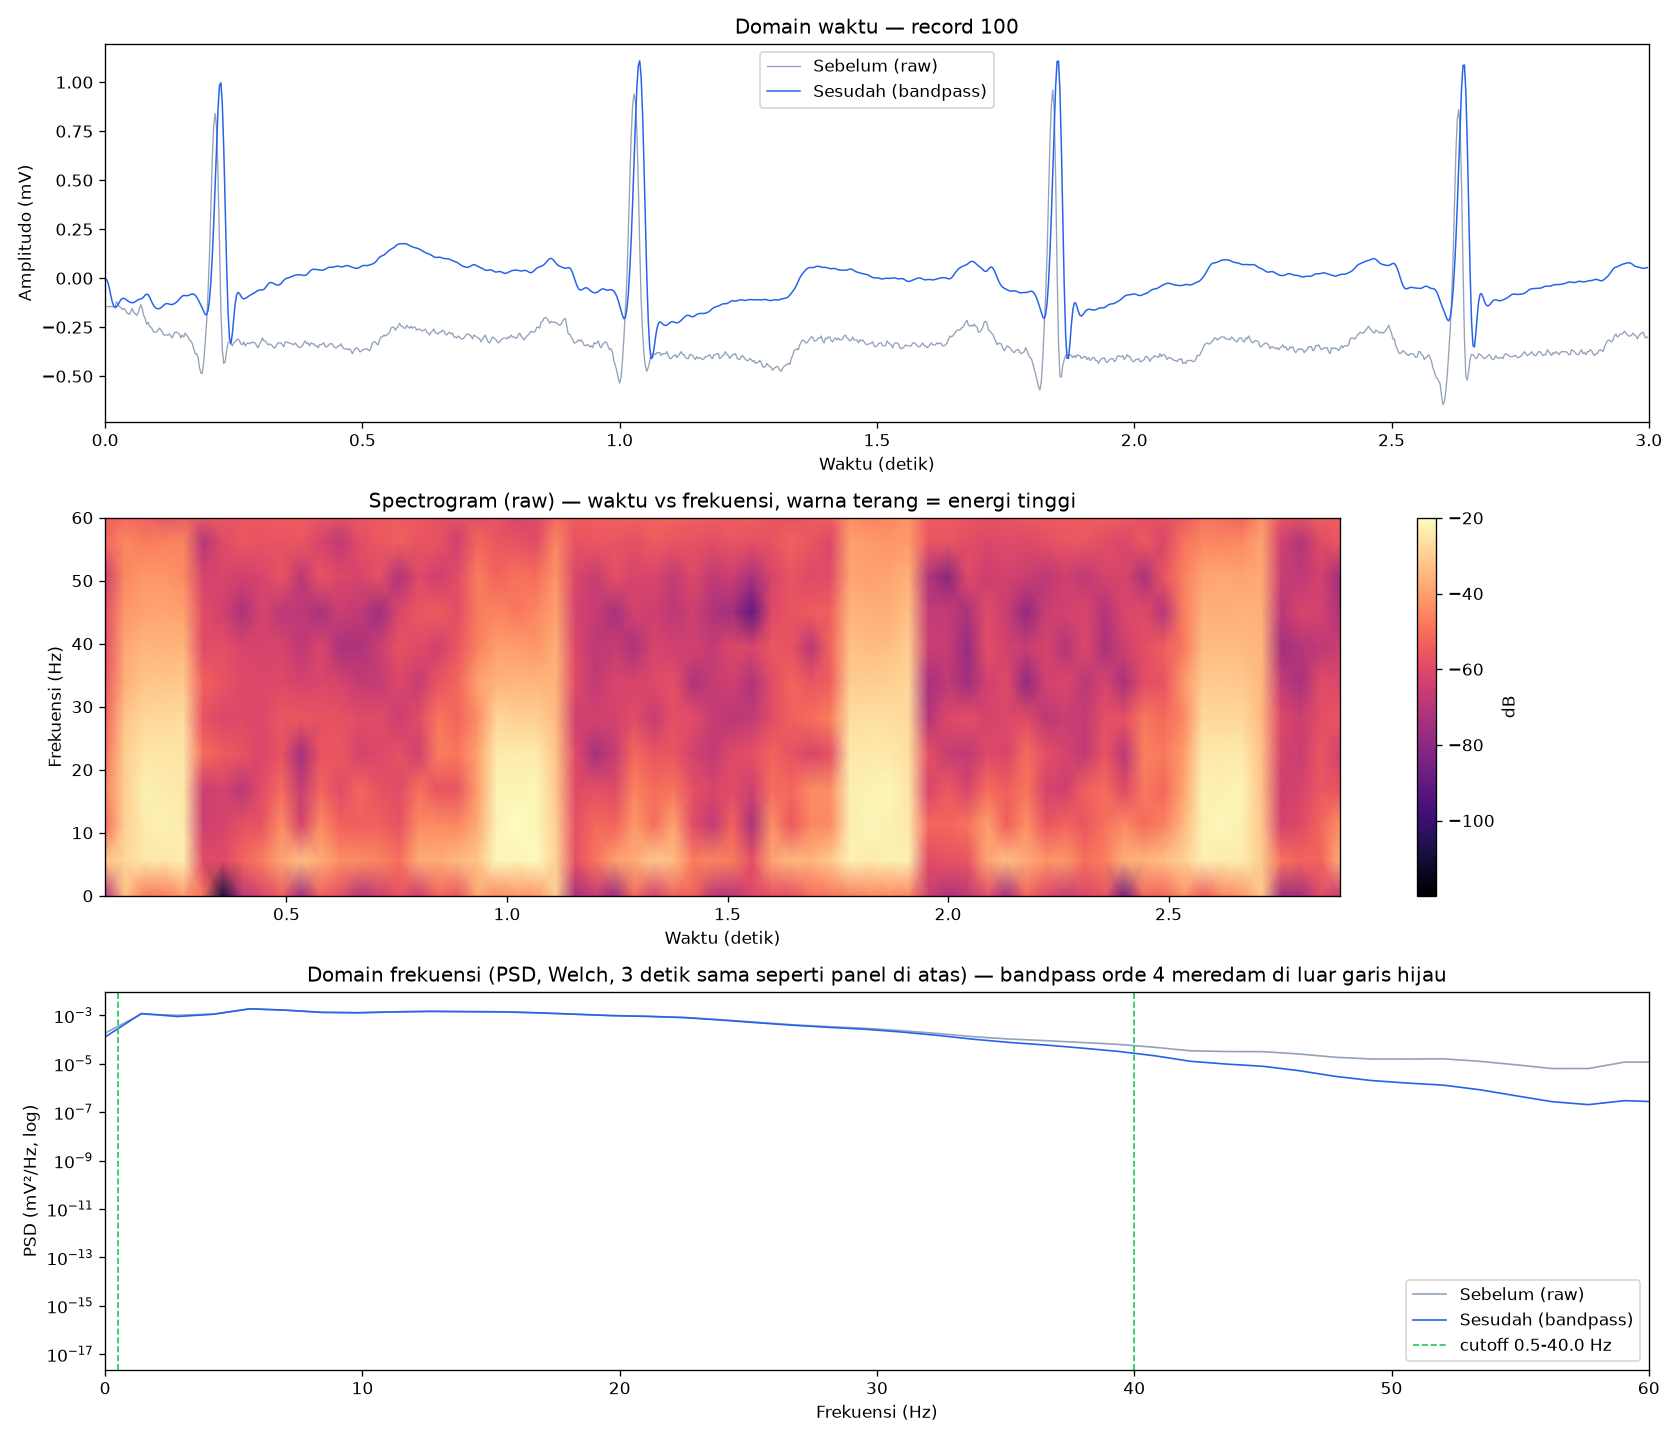
\includegraphics[width=\linewidth,height=0.5\textheight,keepaspectratio]{fase1_100.png}
  \caption{Sinyal rekaman 100 sebelum dan sesudah filter \textit{bandpass} kausal}
  \label{fig:hasil-filter}
\end{figure}

Gambar~\ref{fig:hasil-filter} terdiri atas tiga panel. Pada panel atas, filter memusatkan sinyal di sekitar nol, yaitu rata-rata berubah dari $-0{,}3063$ mV menjadi 0,0000 mV, sedangkan gelombang P, kompleks QRS, dan gelombang T tetap utuh. Simpangan baku sinyal hanya turun dari 0,1932 mV menjadi 0,1840 mV atau sekitar 4,8\%, sehingga filter berperan sebagai pembersih dan bukan pemangkas morfologi. Puncak R pada sinyal tersaring tampak sedikit di kanan puncak pada sinyal mentah, yaitu \textit{group delay} sebesar 4 sampel atau sekitar 11 ms yang sengaja tidak dikoreksi. Panel tengah memperlihatkan spektrogram sinyal mentah dengan energi tertinggi mengumpul pada saat kompleks QRS dan pada frekuensi rendah. Pada panel bawah, kurva kerapatan spektral daya sesudah filter berimpit dengan kurva sebelum filter pada frekuensi rendah, lalu terpisah menjelang 40 Hz dan semakin jauh di bawahnya hingga 60 Hz.
% sumber: gambar laporan/buku-pa/gambar/fase1_100.png (dibuka dan dibaca); perhitungan ulang rekaman 100 (mean -0,3063 -> 0,0000, std 0,1932 -> 0,1840 = -4,8%); model/src/preprocessing.py design_bandpass_sos() (matriks 4 x 6, empat biquad); model/CLAUDE.md Fase 1 dan jebakan "Group delay filter kausal" (4 sampel / 360 Hz = 11,1 ms)

Hasil segmentasi \textit{window} 256 sampel beserta normalisasi \textit{z-score}, yang rancangannya ditunjukkan pada Gambar~\ref{fig:segmentasi}, diperiksa secara numerik pada rekaman 100. Sebanyak 2.273 anotasi menghasilkan 2.271 \textit{window} karena dua detak di tepi rekaman tidak memiliki cukup sampel. Setiap \textit{window} membentang 128 sampel atau sekitar 0,36 detik pada tiap sisi anotasi, dan seluruhnya berukuran 256 sampel dengan rata-rata mendekati nol serta simpangan baku 1,0000 setelah \textit{z-score}. Median indeks puncak R adalah 132 dan seluruh 2.271 \textit{window} memiliki puncak (nilai mutlak terbesar) dalam $\pm$2 sampel dari indeks tersebut.
% sumber: perhitungan ulang rekaman 100 dengan model/src/preprocessing.py segment_beats dan zscore_per_window (2.271 window, bentuk (2271, 256), median indeks puncak 132,0, seluruhnya dalam 132 +- 2, std z-score 1,0000); model/config.py (WIN_PRE 128, FS 360, 128/360 = 0,36 detik)

Ketiga tahap dinilai berjalan sesuai rancangan, sehingga keluarannya dipakai sebagai acuan uji kesetaraan kode C pada butir berikutnya. Verifikasi pada butir ini hanya mencakup rekaman 100 dan 114. Pada rekaman 114, simpangan baku turun dari 0,3755 mV menjadi 0,3480 mV (7,3\%), seluruh 1.879 anotasi menghasilkan \textit{window}, dan 99,8\% \textit{window} memiliki puncak R dalam $\pm$2 sampel dari indeks 132.
% sumber: perhitungan ulang rekaman 114 (std 0,3755 -> 0,3480 = -7,3%, 1.879 window dengan 0 dibuang, 99,8% dalam 132 +- 2); model/CLAUDE.md Fase 1 (std 114 0,3755 -> 0,3480)

\subsubsection{\textit{Port} ke Bahasa C dan Uji Kesetaraan}

Butir ini bertujuan membuktikan bahwa kode C di ESP32-S3 menghitung hal yang sama dengan Python. Pembuktiannya memakai data acuan, yaitu keluaran setiap tahap Python berpresisi \textit{float64} pada 2.400 sampel pertama rekaman 208 DS1 yang disimpan sebagai berkas \textit{header} C dan ikut dikompilasi bersama kode uji. Keluaran kode C berpresisi \textit{float32} dibandingkan dengan acuan tersebut tahap demi tahap dan tidak hanya pada hasil akhir, sehingga tahap yang meleset langsung terlihat. Tahap yang dibandingkan beserta toleransinya ditunjukkan pada Tabel~\ref{tab:uji-kesetaraan-tahap}.
% sumber: firmware/test/golden_ref.h (GOLDEN_N 2400, komentar "golden ini float64 (scipy), device float32", GOLDEN_TOL_FILTER 1e-3, GOLDEN_TOL_ZSCORE 1e-3, GOLDEN_TOL_PROB 2e-2); firmware/test/test_preproc/test_preproc.cpp

\begin{table}[!ht]
  \centering
  \caption{Tahap uji kesetaraan kode C terhadap data acuan Python}
  \label{tab:uji-kesetaraan-tahap}
  \setstretch{1.0}
  \setlength{\tabcolsep}{4pt}
  \renewcommand{\arraystretch}{1.15}
  \small
  \begin{tabular}{|>{\RaggedRight\arraybackslash}p{4.2cm}|>{\RaggedRight\arraybackslash}p{3.0cm}|>{\RaggedRight\arraybackslash}p{3.2cm}|>{\centering\arraybackslash}p{2.2cm}|}
    \hline
    \rowcolor{headgray}
    \textbf{Tahap} & \textbf{Pembanding} & \textbf{Toleransi} & \textbf{Hasil} \\
    \hline
    Filter \textit{bandpass}, sekali jalan & 2.400 sampel & $10^{-3}$ & Lulus \\
    \hline
    Filter \textit{bandpass}, \textit{streaming} per blok 64 sampel & 2.400 sampel & $10^{-3}$ & Lulus \\
    \hline
    Segmentasi dan \textit{z-score} & 9 \textit{window} 256 sampel & $10^{-3}$ & Lulus \\
    \hline
    Rantai utuh dari sinyal mentah ke \textit{z-score} & 9 \textit{window} 256 sampel & $10^{-3}$ & Lulus \\
    \hline
    Fitur interval R-R & 7 detak & $10^{-4}$ & Lulus \\
    \hline
    Deteksi R-\textit{peak} Pan-Tompkins & 11 puncak & 1 sampel & Lulus \\
    \hline
    Penyelarasan puncak R di dalam \textit{window} & Seluruh puncak yang \textit{window}-nya muat & Indeks 132 $\pm$2 sampel & Lulus \\
    \hline
    Probabilitas model INT8 di perangkat & 7 detak & $\leq$ 0,02 dan label identik & Lulus \\
    \hline
  \end{tabular}
\end{table}
% sumber: firmware/test/test_preproc/test_preproc.cpp (test_bandpass, test_bandpass_streaming blok 64, test_window_zscore, test_pipeline_utuh, test_rr_features 1e-4 untuk GOLDEN_RR_FIRST 2 sampai 8 = 7 detak, test_detect_r GOLDEN_N_DETEKSI 11 toleransi 1, test_align_r_menaruh_puncak_di_r_idx R_IDX = 128 + 4 toleransi 2); firmware/test/test_inference/test_inference.cpp (test_inferensi_cocok_dengan_pc, GOLDEN_TOL_PROB, label sama); hasil pio test -e native (23 kasus lulus) dan model/CLAUDE.md HW-1 (pio test -e esp32-s3 16/16 pada 18 Sep 2026); git log f6042b5 (13 Okt 2026, board 29/29, native 23/23)

Berdasarkan Tabel~\ref{tab:uji-kesetaraan-tahap}, seluruh tahap lulus. Uji unit kode C yang dijalankan di komputer tanpa perangkat menghasilkan 23 kasus uji lulus dari 23, dengan 11 di antaranya milik uji preprocessing dan sisanya milik uji MQTT dan INA219. Deteksi R-\textit{peak} di kode C menemukan 11 puncak yang sama dengan Python, seluruhnya dalam toleransi 1 sampel. Selisih filter akibat presisi \textit{float32} tercatat sekitar $2 \times 10^{-4}$ pada amplitudo sekitar 0,4, jauh di bawah toleransi $10^{-3}$, dan uji rantai utuh menunjukkan selisih pada \textit{window} ber-\textit{z-score} tetap di bawah $10^{-3}$. Uji probabilitas model dijalankan terpisah di ESP32-S3.
% sumber: pio test -e native (SUMMARY "23 test cases: 23 succeeded", test_preproc 11 baris PASSED, test_mqtt dan test_ina219 PASSED); firmware/test/golden_ref.h (komentar toleransi filter "terukur ~2e-4 pada amplitudo ~0,4"); model/CLAUDE.md HW-1 dan HW-6 (esp32-s3 16/16 pada 18 Sep 2026); git log f6042b5 (13 Okt 2026, native 23/23, board 29/29)

Kesetaraan pada keluaran akhir dinilai dari probabilitas Aritmia model INT8 pada tujuh detak acuan rekaman 208. Dua detak pertama tidak diuji karena belum memiliki fitur R-R sebelumnya. Keputusan akhir identik pada ketujuh detak, yaitu lima detak berlabel Aritmia berada di atas \textit{threshold} 0,80 dan dua detak berlabel Normal berada di bawahnya. Uji di ESP32-S3 pada 18 September 2026 lulus 16 kasus dari 16, dan rangkaian uji di papan yang sudah diperluas dengan uji perangkat dijalankan ulang pada 13 Oktober 2026 dengan hasil 29 kasus lulus dari 29, termasuk uji probabilitas ini. Catatan uji 18 September hanya mencatat satu detak yang berbeda dari PC, yaitu detak ketujuh pada rekaman 208 yang berlabel Normal dengan probabilitas 0,0820 di perangkat dan 0,0859 di PC. Selisih satu kuantum INT8 ini bernilai 1/256 atau sekitar 0,0039, sekitar seperlima toleransi 0,02, dan tidak mengubah label. Probabilitas keenam detak lainnya tidak disimpan sebagai berkas \textit{log}, sehingga kesamaannya disimpulkan dari catatan tersebut dan dari lulusnya uji pada toleransi 0,02, bukan dari pembacaan nilai per detak.
% sumber: firmware/test/golden_ref.h (golden_prob_int8 indeks 2 sampai 8 = 0,99609375 0,01953125 0,99609375 0,98828125 0,0859375 0,99609375 0,99609375; golden_sym N F V N V V N V V; golden_label 1 0 1 1 0 1 1 untuk indeks 2 sampai 8; detak ketujuh = indeks 6 = 0,0859375; GOLDEN_THRESHOLD 0,8f); firmware/include/model_int8.h (ECG_OUT_SCALE 0.00390625 = 1/256); model/CLAUDE.md HW-1 "angka diperbarui 18 Sep 2026, window 256" (pio test -e esp32-s3 16/16, satu beat beda 1 kuantum INT8, 0,0820 vs 0,0859); 0,00390625 / 0,02 = 0,195. Nilai perangkat per detak tidak tersimpan sebagai berkas log.

Uji kesetaraan ini juga berfungsi sebagai pengaman yang terbukti bekerja. Perbandingan terhadap data acuan inilah yang mengungkap bahwa operasi MEAN pada TensorFlow Lite Micro menghasilkan probabilitas 0,336 di perangkat padahal 0,973 di PC tanpa pesan kesalahan apa pun, sebagaimana tercatat pada Tabel~\ref{tab:perubahan-rancangan}. Keterbatasannya, acuan hanya berasal dari satu rekaman aritmik sepanjang 6,67 detik dengan detak berkelas N, F, dan V, sehingga tidak mencakup kelas S. Kesetaraan diuji dengan sinyal \textit{replay} karena hanya sinyal yang keluaran setiap tahapnya sudah diketahui yang dapat dibandingkan tahap demi tahap, sedangkan filter dan detektor yang diuji adalah kode yang sama yang memproses sinyal tubuh.
% sumber: model/CLAUDE.md jebakan "TFLite Micro menghitung op MEAN beda" (PC 0,9727 vs device 0,3359) dan decision "Model yang dikuantisasi" (PC 0,973 vs device 0,336), selaras dengan tab:perubahan-rancangan di atas; firmware/test/golden_ref.h (golden_sym tanpa S, GOLDEN_N 2400 / 360 = 6,67 detik)

\subsubsection{Alur Hidup dan Beban Komputasi}

Butir ini bertujuan memastikan bahwa seluruh rantai preprocessing dapat berjalan secara \textit{real-time} di ESP32-S3 tanpa kehilangan sampel, yaitu beban rata-rata per sampel lebih kecil daripada 2.778 $\mu$s atau 1/360 detik dan jumlah sampel yang hilang nol. Pengukuran memutar ulang sinyal acuan sampel demi sampel seolah-olah datang dari ADC pada 360 Hz, sedangkan waktu setiap panggilan pemrosesan dicatat dengan penghitung mikrodetik perangkat. Alur hidup yang diuji dimulai dari \textit{timer interrupt} atau \textit{interrupt service routine} (ISR) 360 Hz yang menaruh setiap sampel ke antrean 256 sampel, lalu \textit{loop} utama menguras antrean dan memprosesnya sampai inferensi per detak, sebagaimana ditunjukkan pada Gambar~\ref{fig:alir-preprocessing}.
% sumber: firmware/test/test_inference/test_inference.cpp test_alur_hidup (anggaran 2778 us, micros(), golden_raw diputar per sampel); model/CLAUDE.md HW-3; firmware/src/akuisisi.cpp on_timer() dan loop(); firmware/include/ecg_live.h (ECG_LIVE_RING 4 * ECG_FS, ECG_LIVE_TIAP ECG_FS); model/docs/firmware-walkthrough.md bagian 5c

Hasil pengukuran ditunjukkan pada Tabel~\ref{tab:beban-komputasi}.

\begin{table}[!ht]
  \centering
  \caption{Beban komputasi dan antrean pada alur hidup}
  \label{tab:beban-komputasi}
  \setstretch{1.0}
  \setlength{\tabcolsep}{4pt}
  \renewcommand{\arraystretch}{1.15}
  \small
  \begin{tabular}{|>{\RaggedRight\arraybackslash}p{4.4cm}|>{\RaggedRight\arraybackslash}p{3.4cm}|>{\RaggedRight\arraybackslash}p{4.8cm}|}
    \hline
    \rowcolor{headgray}
    \textbf{Besaran} & \textbf{Nilai} & \textbf{Kondisi Pengukuran} \\
    \hline
    Anggaran waktu per sampel & 2.778 $\mu$s & 1/360 detik \\
    \hline
    Beban rata-rata & 82 $\mu$s per sampel (3,0\% anggaran) & \textit{Replay} sinyal acuan 2.400 sampel di perangkat, model \textit{window} 250 \\
    \hline
    Puncak beban sesaat (\textit{burst}) & 33,4 ms (sekitar 12 kali anggaran) & Deteksi R-\textit{peak} dan inferensi bersamaan, model \textit{window} 250 \\
    \hline
    Kapasitas antrean minimum menurut perhitungan & 13 sampel & Dihitung dari puncak \textit{burst} \\
    \hline
    Antrean saat \textit{burst} & 12 sampel & \textit{Firmware} produksi tanpa elektroda, ADC membaca derau, model \textit{window} 250 \\
    \hline
    Antrean puncak & 21 dari 256 sampel & \textit{Firmware} produksi dengan \textit{replay} sinyal acuan, model \textit{window} 256 \\
    \hline
    Sampel hilang & 0 & Kedua pengukuran \textit{firmware} produksi di atas \\
    \hline
  \end{tabular}
\end{table}
% sumber: model/CLAUDE.md HW-3 (82 us/sampel dari 2778 us = 3,0%, burst 33,4 ms, antrean min 13), HW-4 (antrean 12 saat burst, sampel hilang 0), HW-7 Replay (antrean puncak 21/256, sampel hilang 0); model/docs/firmware-walkthrough.md bagian 5b dan 5c (burst 33.428 us, 12x anggaran satu sampel); 1/360 s = 2.777,8 us

Berdasarkan Tabel~\ref{tab:beban-komputasi}, beban rata-rata hanya 82 $\mu$s per sampel atau 3,0\% dari anggaran 2.778 $\mu$s, sehingga secara rata-rata pemrosesan sangat longgar. Beban tersebut tidak merata. Deteksi R-\textit{peak} yang berjalan atas bufer empat detik dan inferensi detak yang baru ditemukan terjadi bersamaan, sehingga satu sampel dapat memakan 33,4 ms atau sekitar 12 kali anggaran. Apabila ADC dibaca di \textit{loop} yang sama dengan pemrosesan, sekitar 12 sampel akan hilang setiap kali deteksi berjalan dan interval R-R rusak. Karena itu ADC dibaca di ISR dan antrean menampung sedikitnya 13 sampel saat \textit{burst}. Antrean berukuran 256 sampel atau sekitar 0,71 detik memberi ruang jauh lebih besar daripada kebutuhan tersebut. Pada \textit{firmware} produksi, antrean terisi 12 sampel saat \textit{burst}, mendekati 13 hasil perhitungan, dan tidak ada sampel yang hilang. Perangkat mengeluarkan 11 detak per putaran \textit{replay} sepanjang 6,67 detik atau sekitar 1,6 detak per detik dengan pola probabilitas yang identik pada setiap putaran.
% sumber: model/CLAUDE.md HW-3, HW-4, HW-7 Replay (11 beat per putaran 6,67 detik, 11 / 6,67 = 1,65 beat/detik, pola p identik tiap putaran); model/CLAUDE.md jebakan "Beban alur hidup bursty" dan "Menunggu jaringan di dalam loop" (antrean 256 sampel @360 Hz = 711 ms); 256 / 360 = 0,711 detik

Pada pengujian \textit{replay} ditemukan satu kegagalan yang tidak langsung terlihat, yaitu konversi nilai sinyal acuan dari \textit{float} ke \textit{count} ADC di dalam ISR membuat \textit{board} mengalami \textit{panic} bertipe \textit{coprocessor exception} pada detik ke-18,49 sehingga lolos uji singkat. Penyebabnya, ESP32 tidak menyimpan register FPU saat masuk ISR, dan penanganannya adalah mengonversi seluruh sinyal acuan ke tabel bilangan bulat sekali di \textit{setup} dengan tambahan pemakaian RAM dari 21,2\% menjadi 22,7\% untuk tabel sebesar 4.800 byte. Karena \textit{board} yang me-\textit{reset} diam-diam membuat \textit{replay} nonaktif dan pengukuran melaporkan derau ADC, status \textit{replay} diverifikasi dari ayunan sinyal, sebagaimana dibahas pada Subbab~\ref{subsec:validitas-pengukuran}.
% sumber: model/CLAUDE.md jebakan "Float di dalam ISR membunuh ESP32" (EXCCAUSE 0x00000004, detik 18, sim_counts); model/docs/firmware-walkthrough.md (panic di detik 18,49, RAM 21,2% -> 22,7%, sim_counts 4.800 byte); firmware/src/akuisisi.cpp (sim_counts dan on_timer)

Berdasarkan hasil tersebut, alur hidup dinilai memenuhi syarat \textit{real-time} pada sinyal \textit{replay}, yaitu beban rata-rata jauh di bawah anggaran dan sampel hilang nol. Beban rata-rata 82 $\mu$s dan puncak 33,4 ms diukur pada versi model \textit{window} 250 dan belum diukur ulang pada \textit{window} 256. Antrean puncak pada \textit{window} 256 tercatat 21 sampel, lebih tinggi daripada 12 sampel pada versi lama dan setara dengan sekitar 58 ms sampel yang tertahan. Kenaikan ini tidak dapat dijelaskan oleh pertambahan waktu inferensi per detak dari 26,0 ms menjadi 26,6 ms dan penyebabnya belum ditelusuri. Meskipun demikian, 21 sampel baru sekitar 8\% kapasitas antrean 256 sampel dan sampel hilang tetap nol. Pengukuran ini belum mencakup sinyal tubuh dan belum mencakup beban saat WiFi dan MQTT aktif.
% sumber: model/CLAUDE.md HW-1 (26,6 ms per detak, dari 26,0), HW-3 (versi window 250), HW-4 (antrean 12 saat burst), HW-7 Replay (antrean puncak 21/256 pada window 256, sampel hilang 0); 21 / 360 = 0,0583 detik = 58 ms; 21 / 256 = 8,2%

\subsubsection{Uji Perangkat dan Integrasi di Papan}

Butir ini bertujuan memastikan setiap komponen perangkat berfungsi dan jalur \textit{real-time} tetap tidak kehilangan sampel ketika layar, \textit{buzzer}, dan INA219 ikut bekerja, mengikuti rencana pengujian perangkat keras pada Subbab~\ref{sec:rencana-pengujian}. Seluruh rangkaian uji di papan dijalankan pada 13 Oktober 2026 dengan rangkaian berpeta pin PCB, dan hasilnya per rangkaian uji ditunjukkan pada Tabel~\ref{tab:uji-papan}.
% sumber: git log f6042b5 (2026-10-13, "board 29/29, native 23/23") dan 07a5a07 (2026-10-13, "board: 29/29 test perangkat, native 23/23"); firmware/README.md bagian Test (jumlah per suite)

\begin{table}[!ht]
  \centering
  \caption{Hasil rangkaian uji di ESP32-S3 pada 13 Oktober 2026}
  \label{tab:uji-papan}
  \setstretch{1.0}
  \setlength{\tabcolsep}{4pt}
  \renewcommand{\arraystretch}{1.15}
  \small
  \begin{tabular}{|>{\RaggedRight\arraybackslash}p{3.0cm}|>{\centering\arraybackslash}p{1.5cm}|>{\RaggedRight\arraybackslash}p{6.6cm}|>{\centering\arraybackslash}p{1.4cm}|}
    \hline
    \rowcolor{headgray}
    \textbf{Rangkaian Uji} & \textbf{Kasus} & \textbf{Yang Diverifikasi} & \textbf{Hasil} \\
    \hline
    Preprocessing & 11 & Kesetaraan tahap demi tahap terhadap data acuan (Tabel~\ref{tab:uji-kesetaraan-tahap}) & Lulus \\
    \hline
    Inferensi & 5 & Probabilitas model INT8 sama dengan komputer, latensi, dan \textit{tensor arena} & Lulus \\
    \hline
    Integrasi & 5 & Sinyal acuan melalui \textit{timer interrupt}, antrean, deteksi, dan inferensi dengan layar, INA219, dan \textit{buzzer} aktif, yaitu tanpa sampel hilang, detak terdeteksi tiap putaran, laju jantung dalam 3 bpm dari anotasi, dan label sama dengan komputer & Lulus \\
    \hline
    Layar & 2 & Inisialisasi TFT dan transfer SPI satu layar penuh & Lulus \\
    \hline
    ADC dan \textit{lead-off} & 2 & ADC terbaca dan pewaktu menghasilkan 360 sampel per detik & Lulus \\
    \hline
    Tombol & 2 & Ketiga pin berlogika HIGH saat diam dan uji tombol berakhir tepat pada batas waktunya & Lulus \\
    \hline
    \textit{Buzzer} & 1 & Pin tersambung ke pembangkit nada setelah SPI layar terpasang, diam pada logika HIGH & Lulus \\
    \hline
    INA219 & 1 & Modul menjawab di I2C dengan bacaan dalam rentang fisik & Lulus \\
    \hline
    Jumlah & 29 & & 29 lulus \\
    \hline
  \end{tabular}
\end{table}
% sumber: firmware/README.md tabel Test dan baris "board 29 (test_preproc 11, test_inference 5, test_hw_integrasi 5, test_hw_tft 2, test_hw_adc 2, test_hw_tombol 2, test_hw_buzzer 1, test_hw_ina219 1)"; jumlah RUN_TEST per suite di firmware/test/test_*/; firmware/test/test_hw_integrasi/ (n_lewat == 0, PUTARAN 3, HR beda <= 3 bpm, label sama PC); git log f6042b5 (board 29/29)

Berdasarkan Tabel~\ref{tab:uji-papan}, seluruh 29 kasus lulus, dan uji unit di komputer pada tanggal yang sama juga lulus 23 kasus dari 23. Hasil terpenting adalah uji integrasi, karena pengukuran beban pada Tabel~\ref{tab:beban-komputasi} belum mencakup layar dan \textit{buzzer}, sedangkan uji integrasi menunjukkan sampel hilang tetap nol ketika gelombang digambar dan bip dibunyikan selama tiga putaran sinyal acuan. Uji integrasi juga memeriksa laju jantung yang ditampilkan, yaitu berselisih paling banyak 3 bpm dari interval R-R anotasi, dan label setiap detak yang sama dengan komputer. Cakupannya perlu dicatat. Uji otomatis tidak menilai bunyi \textit{buzzer}, warna layar, dan tekanan tombol sungguhan, karena hal tersebut memerlukan pengamatan manusia dan diperiksa melalui menu Tes perangkat yang hasilnya tidak dicatat sebagai berkas. Uji integrasi juga dijalankan tanpa WiFi dan MQTT, sehingga beban radio pada jalur \textit{real-time} hanya teramati pada uji \textit{pipeline} (Subbab~\ref{subsec:hasil-tujuan3}).

Penguncian sesi perekaman pada Subbab~\ref{subsec:antarmuka-perangkat} diuji terpisah dengan menyuntikkan tekanan tombol dan perintah melalui serial ke perangkat yang sedang berjalan, dalam tujuh skenario, yaitu menu terkunci saat merekam, menu tetap terkunci saat dijeda, perubahan sumber, mode daya, pelewatan kalibrasi, WiFi, dan \textit{broker} ditolak saat merekam, perekaman ditolak saat sumber \textit{replay}, perekaman ditolak saat menu terbuka, jeda dan lanjut diakhiri penyimpanan, serta menu dapat dibuka kembali sesudah rekaman disimpan. Ketujuh skenario lulus pada dua putaran dengan sampel hilang nol selama sesi perekaman.
% sumber: git log 5088bb6 (2026-10-13, kunci sesi rekam: uji_alur_rekam.py 7/7 LULUS 2 putaran, sampel hilang 0 selama sesi rekam, pio test esp32-s3 29/29, native 23/23); model/scripts/uji_alur_rekam.py (skenario a-g, tombol disuntik lewat serial t/T); git log f6042b5 (native 23/23); firmware/test/test_hw_integrasi/ (PUTARAN 3, TFT digambar dan buzzer dibunyikan di loop uji, tanpa WiFi); firmware/README.md ("Bunyi buzzer dan isi layar dinilai langsung", menu Tes perangkat); bab4 tab:beban-komputasi (diukur tanpa antarmuka)

\subsubsection{Segmentasi di Perangkat}

Butir ini bertujuan mengukur biaya yang timbul ketika posisi R-\textit{peak} berasal dari detektor Pan-Tompkins di perangkat, bukan dari anotasi seperti pada pelatihan, yaitu berapa banyak detak yang terlewat dan seberapa besar klasifikasi terpengaruh. Pengukuran memakai DS2 dengan rangkaian koreksi posisi yang sama dengan kode C, yaitu kompensasi 38 sampel, penyelarasan ke puncak sinyal dalam $\pm$25 sampel, dan pengurangan \textit{group delay} 4 sampel. Nilai 38 sampel adalah median selisih antara deteksi dan anotasi pada DS1 dengan simpangan baku 13 sampel, sehingga DS2 hanya dipakai untuk mengukur dan tidak untuk memilih parameter. Angka klasifikasi diukur pada model akhir, yaitu \textit{window} 256 sampel dan \textit{threshold} 0,80, dan pada model acuan berukuran \textit{window} 250 sampel dengan \textit{threshold} 0,35 sebagai pembanding, sedangkan angka \textit{sensitivity} detektor tidak melibatkan model.
% sumber: model/docs/segmentasi-deteksi-walkthrough.md §1 dan §3 (offset median 38 sampel dikalibrasi di DS1; dua model: baseline window 90/160 threshold 0,35 dan model berlaku window 128/128 threshold 0,80, diukur ulang 13 Okt 2026 dengan model/scripts/eval_detected_segmentation.py); model/CLAUDE.md decision "Segmentasi on-device" (std 13 sampel); firmware/include/ecg_preproc.h (ECG_PT_OFFSET 38, ECG_PT_REFINE 25, ECG_GROUP_DELAY 4)

Keluaran detektor jatuh di sebelah kanan anotasi pasangannya, yaitu pada garis dasar sesudah kompleks QRS dan bukan pada puncak R. Pada sepuluh detik pertama rekaman 100, seluruh 13 anotasi memiliki 13 deteksi pasangan tanpa deteksi yang terlewat maupun berlebih. Pada keseluruhan rekaman 100, median selisih posisi adalah 40 sampel atau sekitar 0,11 detik, sejalan dengan median 38 sampel dari DS1. Keterlambatan ini sistematis, sehingga dapat dikompensasi dengan satu konstanta, sedangkan penyelarasan ke puncak sinyal menyerap sisa variasinya.
% sumber: perhitungan ulang rekaman 100 dengan model/src/preprocessing.py pan_tompkins_detect (13 anotasi dan 13 deteksi pada 10 detik pertama, median selisih 40 sampel, std 12,1 sampel, 99,9% dalam 38 +- 25; 40/360 = 0,11 detik)

Detektor tidak melewatkan detak dengan peluang yang sama pada semua kelas, sebagaimana ditunjukkan pada Tabel~\ref{tab:sensitivity-detektor}.

\begin{table}[!ht]
  \centering
  \caption{\textit{Sensitivity} detektor Pan-Tompkins per kelas AAMI pada DS2}
  \label{tab:sensitivity-detektor}
  \setstretch{1.0}
  \setlength{\tabcolsep}{4pt}
  \renewcommand{\arraystretch}{1.15}
  \small
  \begin{tabular}{|>{\RaggedRight\arraybackslash}p{4.2cm}|>{\RaggedRight\arraybackslash}p{4.6cm}|>{\centering\arraybackslash}p{3.0cm}|}
    \hline
    \rowcolor{headgray}
    \textbf{Kelas} & \textbf{Keterangan} & \textbf{\textit{Sensitivity}} \\
    \hline
    N & Normal & 0,9614 \\
    \hline
    S & Supraventrikular, datang prematur & 0,6494 \\
    \hline
    V & Ventrikular & 0,9146 \\
    \hline
    F & Fusi & 0,9820 \\
    \hline
    S, V, F, dan Q gabungan & Seluruh aritmia & 0,8296 \\
    \hline
    Seluruh detak & 47.074 terdeteksi dan 2.638 terlewat & 0,9469 \\
    \hline
  \end{tabular}
\end{table}
% sumber: model/docs/segmentasi-deteksi-walkthrough.md bagian 3 dan 4 (47.074 terdeteksi, 2.638 terlewat, sensitivity 0,9469; per kelas N 0,9614, S 0,6494, V 0,9146, F 0,9820, Normal vs Aritmia 0,9614 vs 0,8296); model/scripts/eval_detected_segmentation.py (aritmia = S V F Q); diukur dengan detektor yang sama sebelum window dikunci 256, perhitungannya hanya dari pasangan deteksi dan anotasi sehingga tidak melibatkan model

Berdasarkan Tabel~\ref{tab:sensitivity-detektor}, detektor menemukan 96,14\% detak Normal tetapi hanya 82,96\% detak aritmia, dan kelas S menjadi yang paling sering terlewat dengan \textit{sensitivity} 0,6494. Penjelasan yang paling sesuai bersifat struktural, yaitu detak supraventrikular datang prematur, sedangkan Pan-Tompkins menutup deteksi selama periode refraktori 200~ms sesudah detak sebelumnya, sehingga detak yang datang terlalu cepat berpeluang terblokir. Penjelasan ini belum diuji dengan mengubah periode refraktori.
% sumber: model/docs/segmentasi-deteksi-walkthrough.md §4 (sebab struktural: beat S prematur terblokir periode refraktori 200 ms, PT_REFRACTORY_MS di model/config.py; trade-off refraktori belum diukur)

Dampak segmentasi hasil detektor terhadap klasifikasi ditunjukkan pada Tabel~\ref{tab:segmentasi-deteksi}. \textit{Recall} sistem memakai penyebut seluruh detak aritmia asli, termasuk yang tidak pernah terdeteksi, sedangkan \textit{recall}, \textit{precision}, dan F1 lainnya dihitung pada detak yang terdeteksi.

\begin{table}[!ht]
  \centering
  \caption{Klasifikasi DS2 dengan segmentasi anotasi dan segmentasi hasil detektor}
  \label{tab:segmentasi-deteksi}
  \setstretch{1.0}
  \setlength{\tabcolsep}{4pt}
  \renewcommand{\arraystretch}{1.15}
  \small
  \begin{tabular}{|>{\RaggedRight\arraybackslash}p{3.0cm}|>{\centering\arraybackslash}p{2.2cm}|>{\centering\arraybackslash}p{2.2cm}|>{\centering\arraybackslash}p{2.2cm}|>{\centering\arraybackslash}p{2.2cm}|}
    \hline
    \rowcolor{headgray}
    \textbf{Metrik} & \textbf{Acuan, anotasi} & \textbf{Acuan, detektor} & \textbf{Akhir, anotasi} & \textbf{Akhir, detektor} \\
    \hline
    \textit{Recall} & 0,6661 & 0,6821 & 0,6996 & 0,7279 \\
    \hline
    \textit{Precision} & 0,4919 & 0,4794 & 0,6235 & 0,5869 \\
    \hline
    F1 & 0,5659 & 0,5631 & 0,6594 & 0,6499 \\
    \hline
    \textit{Recall} sistem & 0,6661 & 0,5656 & 0,6996 & 0,6035 \\
    \hline
  \end{tabular}
\end{table}
% sumber: model/docs/segmentasi-deteksi-walkthrough.md §3 tabel A (recall, precision, F1 baseline anotasi/deteksi dan berlaku anotasi/deteksi) dan blok B (recall sistem: baseline 3.084 / 5.453 = 0,5656, berlaku 3.291 / 5.453 = 0,6035); model/artifacts/metrics/fase6b_segmentasi_deteksi.csv memuat baris model acuan (f1 0,565903 / 0,563082, recall_sistem 0,666055 / 0,565560)

Berdasarkan Tabel~\ref{tab:segmentasi-deteksi}, F1 dengan segmentasi detektor berselisih kurang dari 0,01 dari F1 dengan segmentasi anotasi pada kedua model, yaitu 0,6499 dibandingkan 0,6594 pada model akhir, sehingga segmentasi di perangkat tidak merusak klasifikasi selama ketiga koreksi posisi diterapkan. \textit{Recall} sistem model akhir turun dari 0,6996 menjadi 0,6035 karena 3.291 dari 5.453 detak aritmia asli yang tertangkap, dan seluruh penurunan ini berasal dari detak yang tidak pernah sampai ke model. Detektor juga menghasilkan 2.194 deteksi palsu, dan 50,4\% di antaranya diklasifikasi Aritmia oleh model akhir sehingga menambah 1.106 alarm palsu.
% sumber: model/docs/segmentasi-deteksi-walkthrough.md §3 blok B dan C (berlaku: 3.291 dari 5.453 tertangkap; 2.194 deteksi palsu, 50,4% diklasifikasi Aritmia = 1.106 alarm palsu tambahan); 0,6996 - 0,6035 = 0,0961

Butir ini menunjukkan bahwa segmentasi di perangkat layak, dan biayanya terletak pada detektor, bukan pada model. Detektor melewatkan sekitar 5\% detak secara keseluruhan dan sekitar sepertiga detak kelas S, sedangkan klasifikasi pada detak yang terdeteksi setara dengan klasifikasi pada segmentasi anotasi. Ketergantungan model terhadap posisi R yang presisi ditangani dengan latihan ber-\textit{jitter} pada jalur model, yang dipaparkan pada Subbab~\ref{subsec:hasil-tujuan2}.
% sumber: tab:sensitivity-detektor (sensitivity seluruh detak 0,9469, S 0,6494), tab:segmentasi-deteksi; model/docs/jitter-walkthrough.md (latih ulang dengan jitter)

\subsubsection{Akuisisi Sinyal Tubuh}

Butir ini bertujuan menilai apakah modul AD8232 menghasilkan sinyal tubuh yang layak menjadi masukan jalur preprocessing. Rekaman diambil dengan konfigurasi Lead II, elektroda \textit{wet-gel}, dan daya dari \textit{powerbank} agar perangkat tidak tersambung ke jala-jala selama perekaman. Setiap rekaman dinilai dengan lima ukuran, yaitu ayunan sinyal ADC absolut, persentase dengung 50 Hz terhadap energi pita ECG 0,5--40 Hz, jumlah R-\textit{peak} yang ditemukan Pan-Tompkins, proporsi interval R-R yang setara 30 sampai 200 detak per menit, dan autokorelasi energi pita QRS. Pada rekaman yang dijeda, R-\textit{peak}, interval R-R, dan autokorelasi dihitung per segmen sehingga tidak ada interval R-R yang melintasi jeda. Ayunan dalam mV dihitung sebagai ekuivalen masukan AD8232, yaitu jumlah \textit{count} dikalikan 0,757 mV per \textit{count} dari ADC 12-bit dengan atenuasi 11 dB, lalu dibagi \textit{gain} AD8232 sekitar 1.100. Dengan konversi ini, ECG sehat berayun sekitar 2 mV atau sekitar 3.000 \textit{count}, sedangkan ayunan di bawah sekitar 0,1 mV atau 150 \textit{count} berarti tidak ada biopotensial sama sekali. Sebuah rekaman diberi status Berhasil bila dengung kurang dari 15\%, autokorelasi lebih dari 0,25, dan lebih dari 90\% interval R-R berada pada rentang 30 sampai 200 detak per menit. Status Bersinyal diberikan pada rekaman yang berayun sebesar ECG sehat dan memiliki interval R-R yang wajar tetapi tidak memenuhi syarat autokorelasi, sedangkan status Gagal diberikan pada rekaman yang ayunannya di bawah 150 \textit{count}, yang dilaporkan \textit{lead-off} sepanjang rekaman, atau yang dengungnya mendominasi. Jumlah sampel jenuh dilaporkan sebagai keterangan dan bukan sebagai penentu status. Kriteria ini adalah kriteria analisis \textit{offline}, sedangkan gerbang kualitas waktu nyata pada Tabel~\ref{tab:parameter-eksperimen}, yaitu ayunan tersaring 60 \textit{count} dan interval R-R 300--1500 ms, dipakai pada jalur \textit{pipeline}, dan baru syarat ayunannya yang diuji pada Subbab~\ref{subsec:hasil-tujuan3}. Hasil pengujian rekaman resmi ditunjukkan pada Tabel~\ref{tab:kualitas-rekaman}.
% sumber: model/CLAUDE.md jebakan "Telemetri akuisisi bisa berbohong" (konversi 12-bit + atten 11 dB = 0,757 mV/count, gain AD8232 sekitar 1100, EKG sehat sekitar 2 mV sekitar 3000 count, di bawah sekitar 0,1 mV sekitar 150 count tidak ada biopotensial); model/docs/akuisisi-walkthrough.md bagian 1 (USB laptop vs power bank) dan bagian 6 (ukuran dan ambang); firmware/src/perangkat.cpp (ADC_WIDTH_BIT_12, ADC_ATTEN_DB_12, nama lain atenuasi 11 dB); model/scripts/analyze_recording.py (masuk_akal 30-200 bpm; muat() dan analisis_segmen() memisah segmen pada baris jeda)
% sumber: kriteria status: model/scripts/analyze_recording.py main() (dengung < 0,15 dari pita ECG, autokorelasi > 0,25, masuk_akal > 0,9) dan model/docs/akuisisi-walkthrough.md bagian 6; ambang 150 count dari model/CLAUDE.md jebakan "Telemetri akuisisi bisa berbohong"; gerbang waktu nyata AMBANG_AYUN 60 dan RR 300-1500 ms dari baris sumber tab:parameter-eksperimen baris e (bab3.tex gerbang kualitas)

\begin{table}[!ht]
  \centering
  \caption{Kualitas rekaman AD8232 pada pengujian rekaman resmi (nama rekaman memakai jam penarikan berkas)}
  \label{tab:kualitas-rekaman}
  \setstretch{1.0}
  \setlength{\tabcolsep}{2.5pt}
  \renewcommand{\arraystretch}{1.15}
  \footnotesize
  \begin{tabular}{|>{\centering\arraybackslash}p{1.5cm}|>{\centering\arraybackslash}p{1.2cm}|>{\centering\arraybackslash}p{1.9cm}|>{\centering\arraybackslash}p{1.5cm}|>{\centering\arraybackslash}p{1.1cm}|>{\centering\arraybackslash}p{1.5cm}|>{\centering\arraybackslash}p{1.2cm}|>{\RaggedRight\arraybackslash}p{2.3cm}|}
    \hline
    \rowcolor{headgray}
    \textbf{Rekaman} & \textbf{Durasi (detik)} & \textbf{Ayunan (\textit{count} / mV)} & \textbf{Dengung (\%)} & \textbf{R-\textit{peak}} & \textbf{Auto-\newline korelasi} & \textbf{BPM Wajar (\%)} & \textbf{Status} \\
    \hline
    \multicolumn{8}{|l|}{\textit{Sesi} \PlaceholderData{tanggal sesi dan rangkaian}} \\
    \hline
    \multicolumn{8}{|>{\RaggedRight\arraybackslash}p{13.3cm}|}{\PlaceholderData{satu baris per rekaman resmi berisi jam penarikan, durasi, ayunan dalam \textit{count} dan mV, dengung 50 Hz, jumlah R-\textit{peak}, autokorelasi, BPM wajar, serta status Berhasil, Bersinyal, atau Gagal beserta jumlah sampel jenuh}} \\
    \hline
  \end{tabular}
\end{table}
% PLACEHOLDER-DATA tab-kualitas-rekaman: satu baris per rekaman resmi (>= 13 Okt 2026), dikelompokkan per sesi (baris \multicolumn tanggal sesi dan rangkaian). Prosedur: model/docs/akuisisi-walkthrough.md §3-§6. Skrip: make pull lalu make analisis FILE=data/recordings/<nama>.csv (model/scripts/analyze_recording.py). Kolom: Rekaman (jam tarik HHMM) | Durasi = n/360 | Ayunan = max-min ADC mentah, mV = count x 0,757 / 1100 | Dengung = energi 49-51 Hz per energi 0,5-40 Hz | R-peak Pan-Tompkins | Autokorelasi = kekuatan puncak denyut_autokorelasi | BPM wajar = persen RR setara 30-200 bpm | Status menurut kriteria paragraf di atas + jumlah sampel jenuh (0 atau 4095) dan lead-off dari header "lepas=". Hapus kedua baris \multicolumn placeholder setelah diisi
% sumber: rekaman uji coba 10 Sep - 11 Okt 2026 tidak dimasukkan (arsip model/data/arsip/rekaman-uji-coba/, bukan hasil)

Berdasarkan Tabel~\ref{tab:kualitas-rekaman}, \PlaceholderData{jumlah rekaman berstatus Berhasil, Bersinyal, dan Gagal dari seluruh rekaman resmi}. \PlaceholderData{uraian rekaman Berhasil, yaitu ayunan dalam \textit{count} dan mV, jumlah R-\textit{peak} per durasi dan setara detak per menit, autokorelasi beserta BPM periode dominannya, dengung, dan jumlah sampel jenuh dibandingkan terhadap kriteria}. \PlaceholderData{uraian rekaman Bersinyal dan Gagal beserta ukuran yang tidak memenuhi kriteria}.
% PLACEHOLDER-DATA uraian-kualitas-rekaman: diisi dari keluaran terminal make analisis FILE=data/recordings/<nama>.csv untuk setiap baris tab:kualitas-rekaman (baris ADC/clipping, dengung 50Hz, denyut autokorelasi @ bpm, R-peak, BPM); ambang 0,25 dan 15% dari model/docs/akuisisi-walkthrough.md §6

Rekaman berhasil dan rekaman gagal dibandingkan secara visual pada Gambar~\ref{fig:rekaman-berhasil}, yang menampilkan rekaman \PlaceholderData{nama rekaman Berhasil} pada bagian atas dan rekaman \PlaceholderData{nama rekaman Gagal} pada bagian bawah.

% PLACEHOLDER-DATA fig-rekaman-berhasil: plot data (bukan ilustrasi), dua grafik hasil make analisis FILE=data/recordings/<nama>.csv -> model/artifacts/metrics/akuisisi/akuisisi_<nama>.png, satu rekaman Berhasil (atas) dan satu rekaman Gagal (bawah) dari pengujian resmi. Salin dengan scripts/export_artifacts.sh --laporan setelah daftar figurnya diperbarui. Ganti \fbox dengan dua \includegraphics[height=0.3\textheight,keepaspectratio]{akuisisi_<nama>.png} dipisah \\[2pt]. Bila tidak ada rekaman Gagal, tampilkan satu rekaman Berhasil dan sesuaikan caption serta paragraf
\begin{figure}[!ht]
  \centering
  \fbox{\parbox[c][5cm][c]{0.85\linewidth}{\centering\small
    \PlaceholderData{grafik analisis rekaman Berhasil di atas dan rekaman Gagal di bawah, masing-masing tiga panel}}}
  \caption{Rekaman AD8232 yang berhasil (atas) dan yang gagal (bawah), enam detik pertama}
  \label{fig:rekaman-berhasil}
\end{figure}

Gambar~\ref{fig:rekaman-berhasil} terdiri atas dua kelompok yang masing-masing memiliki tiga panel, yaitu ADC mentah, sinyal sesudah \textit{bandpass} dengan garis merah pada setiap R-\textit{peak} hasil Pan-Tompkins, dan spektrum dengan pita merah untuk dengung 50 Hz serta pita hijau untuk pita ECG. \PlaceholderData{pengamatan per panel pada rekaman Berhasil, yaitu puncak QRS dan garis dasar dalam \textit{count}, jumlah R-\textit{peak} dalam enam detik beserta jarak antarpuncak, dan puncak 50 Hz pada spektrum}. \PlaceholderData{pengamatan per panel pada rekaman Gagal}. Filter \textit{bandpass} hanya meredam 50 Hz sebesar 9,3 dB, yaitu penguatan 0,342, sehingga dengung yang masuk ke ADC tetap dapat tampak sebagai gerigi pada garis dasar sesudah penyaringan.
% PLACEHOLDER-DATA pengamatan-grafik-rekaman: dibaca langsung dari grafik akuisisi_<nama>.png rekaman resmi pada Gambar fig:rekaman-berhasil
% sumber: tiga panel dari model/scripts/analyze_recording.py (ADC mentah, bandpass + garis R-peak, spektrum pita 50 Hz merah dan pita EKG hijau; model/docs/akuisisi-walkthrough.md §5); model/docs/akuisisi-walkthrough.md §2 (bandpass meredam 50 Hz -9,3 dB, gain 0,342) dan perhitungan ulang sosfreqz atas model/src/preprocessing.py design_bandpass_sos() pada 50 Hz (gain 0,3422 = -9,31 dB)

Prosedur perekaman pada pengujian ini, yaitu catu daya \textit{powerbank}, elektroda baru yang ditempel sekali, dan penilaian kualitas dari ayunan ADC absolut, disusun dari perekaman uji coba selama pengembangan. Perekaman uji coba tersebut memakai rangkaian yang masih berubah sehingga tidak dilaporkan sebagai hasil. \PlaceholderData{penelusuran penyebab rekaman Gagal pada pengujian resmi dengan mengubah satu variabel per percobaan, bila ada rekaman Gagal}.
% PLACEHOLDER-DATA penyebab-rekaman-gagal: diisi bila pengujian resmi menghasilkan rekaman Gagal; tabel gejala dan pemeriksaan di model/docs/akuisisi-walkthrough.md §7. Hapus kalimat placeholder bila seluruh rekaman Berhasil
% sumber: model/docs/akuisisi-walkthrough.md §1 (powerbank, elektroda sekali tempel), §6 (ayunan ADC absolut sebagai wasit) dan §8 (rekaman uji coba, arsip model/data/arsip/rekaman-uji-coba/)

Rekaman gagal juga dapat memperlihatkan jebakan telemetri. Pan-Tompkins tetap melaporkan R-\textit{peak} karena ambangnya adaptif terhadap sinyal yang ada, sehingga keadaan tanpa sinyal bukan kondisi yang dikenalinya. Pada \textit{firmware}, tanpa elektroda dan tanpa \textit{replay}, alat mengeluarkan sekitar 2 detak per detik dengan 57\% di antaranya diklasifikasi Aritmia. \PlaceholderData{contoh rekaman Gagal pada pengujian resmi yang tetap melaporkan R-\textit{peak}, yaitu jumlah R-\textit{peak}, durasi, dan setara detak per menit, bila ada}. Keberadaan detak karena itu tidak dapat dijadikan penentu kualitas sinyal, dan ayunan ADC absolut dipakai sebagai gerbang kualitas pada jalur \textit{pipeline} (Subbab~\ref{subsec:hasil-tujuan3}).
% PLACEHOLDER-DATA rekaman-gagal-rpeak: dari baris "R-peak N dalam T detik" keluaran make analisis atas rekaman resmi berstatus Gagal; hapus kalimat bila tidak ada
% sumber: model/CLAUDE.md jebakan "Tanpa elektroda, alat mengarang aritmia: ~2 beat/detik, 57% ARITMIA" dan "Telemetri akuisisi bisa berbohong"; model/docs/akuisisi-walkthrough.md bagian 6

Dengan demikian, \PlaceholderData{kesimpulan kelayakan sinyal tubuh sebagai masukan jalur preprocessing, yaitu jumlah rekaman yang memenuhi kriteria kualitas dari jumlah sesi dan rangkaian yang dipakai}.
% PLACEHOLDER-DATA kesimpulan-akuisisi: diturunkan dari tab:kualitas-rekaman setelah terisi; status Tujuan 1 pada tab:ketercapaian dan subsec:analisis-tujuan1 ikut dinilai ulang

\subsection{Jalur Model TinyML \textit{On-Device} (Tujuan 2)}
\label{subsec:hasil-tujuan2}

Subbab ini menjawab Tujuan 2 pada Subbab~\ref{sec:tujuan}, yaitu menerapkan model TinyML terkuantisasi INT8 untuk deteksi aritmia secara \textit{on-device} pada ESP32-S3 tanpa ketergantungan pada komputasi \textit{cloud}. Targetnya mengikuti Tabel~\ref{tab:pengujian-model}, yaitu kualitas klasifikasi DS2 pada \textit{threshold} hasil kalibrasi VAL, selisih \textit{recall} akibat kuantisasi di bawah 0,02, latensi di bawah interval antardetak, model di bawah 25 KB yang muat di memori, serta daya per mode operasi. Hasilnya dipaparkan dalam tujuh butir berikut.
% sumber: laporan/buku-pa/bab/bab1.tex Tujuan butir 2; laporan/buku-pa/bab/bab3.tex tab:pengujian-model (|delta recall| < 0,02, ukuran < 25 KB, latensi < interval antardetak, daya per mode operasi)

\subsubsection{Pelatihan dan Pemilihan Titik Operasi}

Butir ini bertujuan memperoleh model dan titik operasinya dengan \textit{epoch} dan \textit{threshold} yang ditentukan hanya dari VAL. Model \textit{hybrid} dengan 6.417 parameter dilatih pada 121.857 baris DS1, yaitu 40.619 detak beserta dua salinan ber-\textit{jitter}, dengan konfigurasi pada Subbab~\ref{subsec:model-tinyml}, sedangkan VAL sebanyak 31.047 baris dipakai untuk \textit{early stopping} dan kalibrasi \textit{threshold}. Perjalanan pelatihan ditunjukkan pada Gambar~\ref{fig:hasil-latih}.
% sumber: laporan/buku-pa/bab/bab4.tex tab:dataset dan tab:perubahan-rancangan (DS1 latih 121.857 = 40.619 x 3, VAL 31.047, 6.417 parameter); model/config.py (BATCH_SIZE 64, EARLY_STOP_PATIENCE 8, EARLY_STOP_MONITOR val_auc)

\begin{figure}[H]
  \centering
  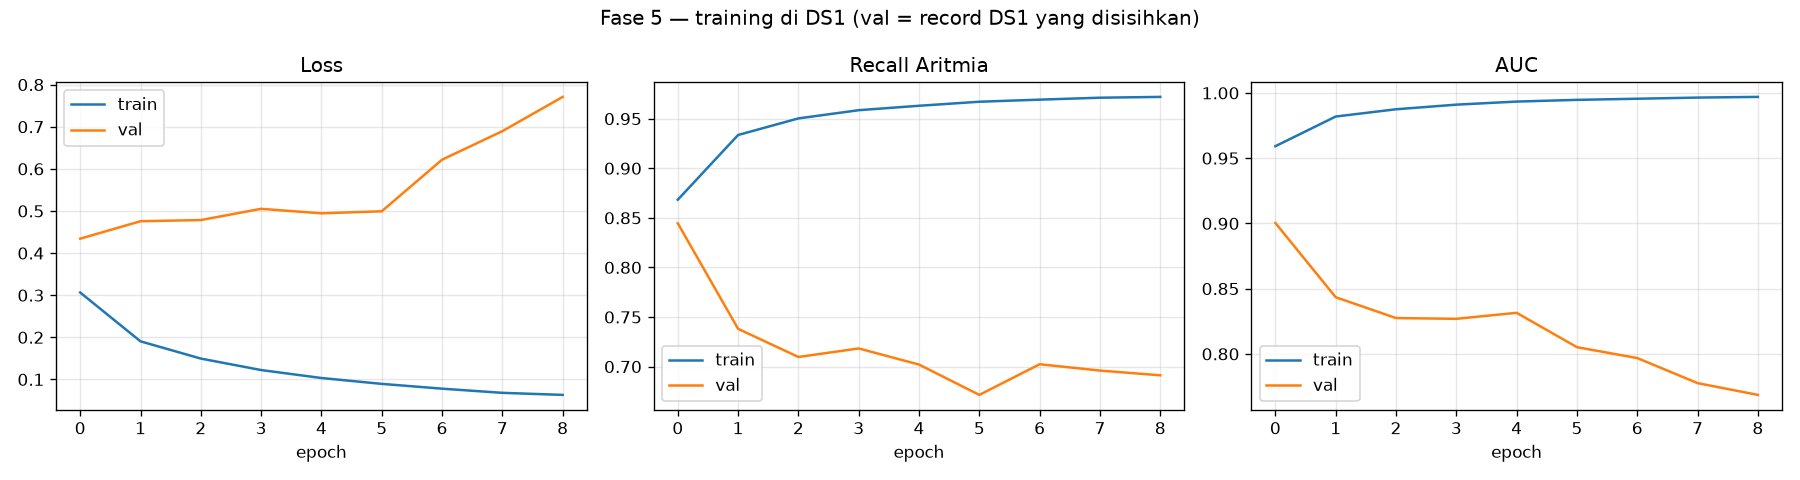
\includegraphics[width=\linewidth,keepaspectratio]{fase5_training.png}
  \caption{Kurva \textit{loss}, \textit{recall} Aritmia, dan AUC selama pelatihan model pada DS1}
  \label{fig:hasil-latih}
\end{figure}

Gambar~\ref{fig:hasil-latih} memperlihatkan kurva data latih berwarna biru yang terus membaik. Pada kurva VAL berwarna jingga, \textit{loss} naik dari sekitar 0,43 menjadi sekitar 0,77, \textit{recall} pada \textit{threshold} bawaan 0,5 turun dari sekitar 0,85 menjadi sekitar 0,69, dan AUC memuncak sekitar 0,90 pada \textit{epoch} 0, yaitu \textit{epoch} pertama karena penomoran dimulai dari nol, lalu turun hingga sekitar 0,77 pada \textit{epoch} 8. Karena AUC validasi tidak pernah melampaui nilai \textit{epoch} 0, \textit{early stopping} mengembalikan bobot \textit{epoch} 0, sehingga model yang dipakai adalah hasil satu \textit{epoch} pelatihan. Penyebabnya diduga jumlah langkah gradien, karena augmentasi tiga salinan membuat satu \textit{epoch} berisi 1.905 langkah, yaitu 121.857 baris dibagi ukuran \textit{batch} 64, yang sudah cukup bagi 6.417 parameter untuk menyesuaikan diri dengan data latih. \textit{Threshold} kemudian dipilih dari \textit{sweep} 0,05 sampai 0,95 pada VAL dengan kriteria F1 maksimum dan \textit{recall} sebagai penentu bila selisih F1 kurang dari 0,005. Nilai 0,80 memberi F1 VAL tertinggi sebesar 0,6917 dan 0,85 memberi 0,6886 dengan selisih kurang dari 0,005, sehingga keduanya dibandingkan dengan \textit{recall} dan 0,80 menang dengan 0,6539 dibandingkan 0,6141.
% sumber: gambar laporan/buku-pa/gambar/fase5_training.png (dibuka dan dibaca, sumbu epoch 0 sampai 8, biru = train, jingga = val; val loss 0,43 ke 0,77, val recall 0,85 ke 0,69, val AUC 0,90 ke 0,77); model/src/train.py (metrics.Recall dengan threshold bawaan 0,5, EarlyStopping restore_best_weights); model/docs/arsip/2026-09-19-faseG-changelog.md bagian 2 (1.905 langkah gradien per epoch, val_auc memuncak di epoch 0); 121.857 / 64 = 1.904,02 sehingga 1.905 langkah
% sumber: model/scripts/calibrate_threshold.py (sapuan 0,05-0,95 langkah 0,05, F1_TIE_MARGIN 0,005, pilih recall tertinggi di antara kandidat); model/artifacts/metrics/fase5_threshold_sweep.csv (0,80: f1 0,691724 recall 0,653920; 0,85: f1 0,688583 recall 0,614085); model/config.py THRESHOLD = 0.80

\subsubsection{Evaluasi pada DS2}

Butir ini bertujuan mengukur kemampuan model pada pasien yang tidak pernah dilihat saat pelatihan. Model \textit{float32} dievaluasi pada 49.656 detak DS2 dari 22 pasien, termasuk 5.450 detak Aritmia, pada \textit{threshold} 0,80 dengan metrik pada Persamaan~\ref{eq:metrik} di Subbab~\ref{subsec:evaluasi-metrik}, dan hasilnya ditunjukkan pada Tabel~\ref{tab:hasil-ds2}.
% sumber: model/artifacts/metrics/fase6_per_record_fp32.csv (22 rekaman, jumlah n_beat 49.656, jumlah n_aritmia 5.450); model/scripts/eval_fp32.py (threshold dari config.THRESHOLD, tidak disetel di DS2)

\begin{table}[!ht]
  \centering
  \caption{Hasil klasifikasi model \textit{float32} pada DS2 dengan \textit{threshold} 0,80}
  \label{tab:hasil-ds2}
  \setstretch{1.0}
  \setlength{\tabcolsep}{4pt}
  \renewcommand{\arraystretch}{1.15}
  \small
  \begin{tabular}{|>{\RaggedRight\arraybackslash}p{2.6cm}|>{\centering\arraybackslash}p{2.2cm}|>{\RaggedRight\arraybackslash}p{4.4cm}|>{\centering\arraybackslash}p{2.2cm}|}
    \hline
    \rowcolor{headgray}
    \textbf{Sel} & \textbf{Jumlah Detak} & \textbf{Metrik} & \textbf{Nilai} \\
    \hline
    TP & 3.813 & \textit{Recall} & 0,6996 \\
    \hline
    FN & 1.637 & \textit{Precision} & 0,6235 \\
    \hline
    FP & 2.302 & \textit{Specificity} & 0,9479 \\
    \hline
    TN & 41.904 & F1 & 0,6594 \\
    \hline
    \multicolumn{2}{|l|}{} & AUC & 0,9334 \\
    \hline
    \multicolumn{2}{|l|}{} & \textit{Accuracy} (bukan acuan) & 0,9207 \\
    \hline
  \end{tabular}
\end{table}
% sumber: model/artifacts/metrics/fase6_metrics_fp32.csv (threshold 0.80, tp 3813, fn 1637, fp 2302, tn 41904, accuracy 0,920674, precision 0,623549, recall 0,699633, specificity 0,947926, f1 0,659403, auc 0,933448)

Berdasarkan Tabel~\ref{tab:hasil-ds2}, model mendeteksi 3.813 dari 5.450 detak Aritmia dan mengenali 41.904 dari 44.206 detak Normal. \textit{Precision} 0,6235 berarti sekitar 38\% alarm adalah alarm palsu, sedangkan AUC 0,9334 menunjukkan pemisahan kelas yang tidak bergantung pada \textit{threshold}. \textit{Accuracy} 0,9207 hanya sekitar 3 poin di atas hasil menebak Normal untuk seluruh detak (Subbab~\ref{subsec:evaluasi-metrik}). Per kelas AAMI, yang dihitung ulang dengan menjalankan model \textit{float32} pada DS2 beserta simbol AAMI-nya, \textit{recall} kelas V, S, dan F masing-masing 0,9248, 0,4390, dan 0,0670 dari 3.219, 1.836, dan 388 detak, sedangkan 7 detak kelas Q tidak ditampilkan. Kelas S lemah karena bentuk kompleks QRS-nya mirip Normal dan pembedanya terletak pada waktu kedatangan serta gelombang P, yang menjadi alasan cabang ritme ditambahkan.
% sumber: fase6_metrics_fp32.csv; 41.904 + 2.302 = 44.206 detak Normal; 2.302 / (3.813 + 2.302) = 0,3765; tebak Normal 44.206 / 49.656 = 0,8902 dan 0,9207 - 0,8902 = 0,0305; per kelas dari perhitungan ulang dengan model/.venv atas model/artifacts/model_fp32.keras pada model/data/processed/test.npz, simbol dari model/data/processed/per_record/<rekaman>.npz dipetakan dengan config.AAMI_MAP, threshold 0,80 (S 806/1.836 = 0,4390, V 2.977/3.219 = 0,9248, F 26/388 = 0,0670, Q 4/7, jumlah terdeteksi 3.813 = TP)

\textit{Recall} per pasien dihitung pada 21 rekaman yang memiliki aritmia, karena rekaman 212 tidak memuat aritmia. Mediannya 0,9167, tetapi \textit{recall} tingkat detak terseret dua rekaman, yaitu rekaman 232 yang berisi 1.381 detak S dengan \textit{recall} 0,3541 dan rekaman 213 yang didominasi 362 detak F dengan \textit{recall} 0,2246. Keduanya menyumbang 83,4\% dari 1.637 detak terlewat. Keterbatasannya, \textit{epoch} dan \textit{threshold} hanya memakai VAL, tetapi ukuran \textit{window} dan jumlah salinan \textit{jitter} dipilih dari ablasi yang dinilai pada DS2, sehingga DS2 bukan tolok ukur yang tidak tersentuh untuk kedua keputusan itu dan angkanya berpotensi sedikit optimistis.
% sumber: model/.venv/bin/python atas model/artifacts/metrics/fase6_per_record_fp32.csv (aturan: hanya rekaman n_aritmia > 0, rekaman 212 n_aritmia 0 dikeluarkan; 21 rekaman, median recall 0,9167, 11 rekaman >= 0,9; 232 recall 0,3541 n_aritmia 1.381 fn 892; 213 recall 0,2246 n_aritmia 610 fn 473; 1.365 / 1.637 = 0,834; 1.381 / 5.450 = 0,253); komposisi kelas dari model/data/processed/per_record/232.npz (S 1.381, N 397) dan 213.npz (F 362, V 220, S 28); model/docs/arsip/2026-09-18-robustness-changelog.md (ablasi window dan salinan dinilai F1 DS2, threshold dari VAL)

\subsubsection{Ketahanan terhadap \textit{Error} Segmentasi}

Butir ini bertujuan mengukur penyimpangan posisi R hasil detektor terhadap anotasi beserta dampaknya pada model. Rangkaian yang identik dengan kode C, yaitu Pan-Tompkins, kompensasi 38 sampel, penyelarasan ke puncak dalam $\pm$25 sampel, dan pengurangan \textit{group delay} 4 sampel, dijalankan pada DS1 karena sebarannya kemudian dipakai untuk melatih. Selisih setiap deteksi terhadap anotasinya, yang disebut residu, ditunjukkan pada Gambar~\ref{fig:residu-jitter}.
% sumber: model/docs/jitter-walkthrough.md bagian 2 (rantai pan_tompkins_detect, haluskan, pair_detected, DS1 saja); firmware/include/ecg_preproc.h (ECG_PT_OFFSET 38, ECG_PT_REFINE 25, ECG_GROUP_DELAY 4)

\begin{figure}[H]
  \centering
  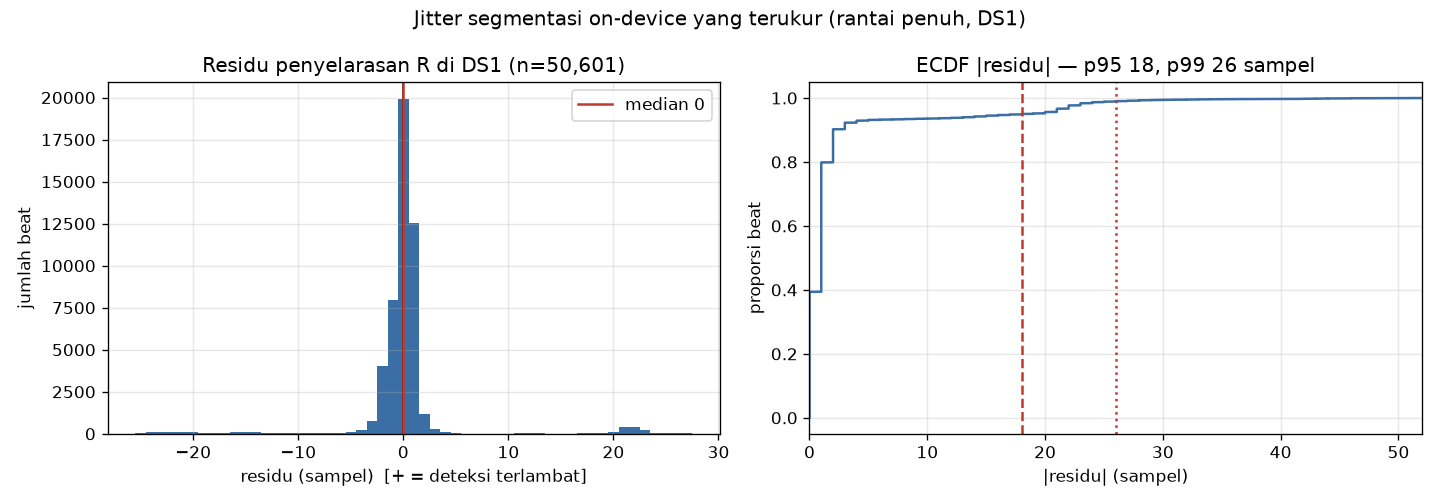
\includegraphics[width=\linewidth,keepaspectratio]{jitter_residu.png}
  \caption{Sebaran residu posisi R-\textit{peak} hasil detektor terhadap anotasi pada DS1}
  \label{fig:residu-jitter}
\end{figure}

Gambar~\ref{fig:residu-jitter} memperlihatkan histogram residu 50.601 pasangan deteksi dan anotasi pada panel kiri serta fungsi distribusi kumulatif empiris (ECDF) nilai mutlaknya pada panel kanan. Intinya sangat tajam di sekitar median 0, yaitu 79,9\% detak meleset paling banyak 1 sampel, tetapi ekornya berat dengan persentil ke-95 dan ke-99 sebesar 18 dan 26 sampel yang ditandai garis vertikal, serta residu terbesar 54 sampel atau sekitar 150 ms. Ekor ini terkumpul pada rekaman berderau 108, 203, dan 207. Bentuk ini berbeda dari \textit{jitter} seragam $\pm$18 sampel pada Dias et al.~\cite{dias_2021}, sehingga augmentasi mengambil ulang residu terukur (Subbab~\ref{subsec:augmentasi-jitter}).
% sumber: gambar laporan/buku-pa/gambar/jitter_residu.png (dibuka dan dibaca); model/artifacts/metrics/jitter/residu_ds1.npy (50.601 residu, median 0, |r| <= 1 0,7985, |r| <= 2 0,9022, p95 18, p99 26, maks 54); model/artifacts/metrics/jitter/jitter_residu.csv (std 108 14,771, 203 10,792, 207 17,434); 54 / 360 = 0,150 detik; model/docs/jitter-walkthrough.md bagian 2 (paper memakai jitter seragam delta <= 18 sampel)

Pada model lama, yaitu \textit{window} 250 sampel tanpa augmentasi dengan \textit{threshold} 0,35, menggeser posisi R pada DS2 mengikuti sebaran ini menurunkan F1 dari 0,5659 menjadi 0,4534, sedangkan AUC hanya turun dari 0,8866 menjadi 0,8586, sehingga urutan probabilitas nyaris utuh dan yang rusak adalah titik operasinya. Pergeseran seragam 4 sampel saja sudah menurunkan F1 menjadi 0,3170, karena tiga lapisan \textit{max pooling} berukuran 2 membuat pergeseran 4 sampel setara setengah \textit{bin pooling}. Model karena itu dilatih ulang dengan dua salinan DS1 ber-\textit{jitter} empiris, dan pada model hasil latih ulang tersebut F1 dengan segmentasi detektor hanya berselisih 0,0095 dari F1 dengan segmentasi anotasi (Tabel~\ref{tab:segmentasi-deteksi}).

% sumber: rerata lima seed dari model/artifacts/metrics/jitter/sweep_jitter_dasar.csv (n 49.654 = DS2 versi window 250; delta 0: f1 0,5659 auc 0,8866; delta 4 seragam: f1 0,3170; empiris: f1 0,4534 auc 0,8586); model/docs/jitter-walkthrough.md bagian 4 (model Fase 5 threshold 0,35, kerusakan pada titik operasi); model/CLAUDE.md jebakan "Model runtuh kalau R-peak meleset 4 sampel" (stride total 8)

\subsubsection{Ablasi dan Keputusan Rancangan}

Butir ini bertujuan memastikan setiap perubahan rancangan didukung pengukuran. Setiap varian melewati rantai yang sama, yaitu menyusun DS1 sesuai varian, melatih, mengalibrasi \textit{threshold} pada VAL, lalu mengukur DS2, dengan satu pengaturan yang diubah, paling sedikit tiga \textit{seed}, dan hasil berupa rerata beserta setengah rentang. Selisih F1 di bawah 0,04 tidak dianggap bermakna, karena penjadwalan \textit{thread} oneDNN membuat hasil berubah walaupun \textit{seed} sama, dan rerata tiga \textit{seed} konfigurasi terkunci pun bergeser dari 0,6911 menjadi 0,6535 saat diulang pada pengulangan kedua. F1 model akhir sebesar 0,6594 berada dalam rentang pengulangan kedua, yaitu 0,6261 sampai 0,6821. Vonis Dikunci diberikan pada varian yang dipakai, Ditolak pada varian yang tidak dipakai karena lebih buruk, menukar kelas yang lebih penting, atau menambah biaya tanpa selisih bermakna, dan Bukan sinyal pada selisih F1 di bawah ambang tanpa bukti manfaat maupun biaya tambahan. Sebagian varian dilatih dengan rekaman SVDB atau INCART di luar data uji SVDB dan INCART, tetapi model akhir hanya dilatih dengan DS1 MIT-BIH. Hasil yang menentukan keputusan dirangkum pada Tabel~\ref{tab:ablasi}.
% sumber: model/docs/jitter-walkthrough.md bagian 5 (rantai ablasi, threshold per varian dari VAL, ukur DS2); model/scripts/ringkas_ablasi.py (SEED_MINIMAL 3, rerata dan setengah-rentang, AMBANG = 0.04); model/docs/arsip/2026-09-18-robustness-changelog.md bagian B2 (0,6209 vs 0,5882); keluaran ringkas_ablasi.py (w128b 0,6911, t8_lr1e3 0,6535); model/artifacts/metrics/ablasi/ablasi.csv (seed 42, 7, 13, ditambah 21, 34, 55 pada sebagian varian; t8_lr1e3 per seed 0,626084, 0,682129, 0,652266); model/artifacts/metrics/fase6_metrics_fp32.csv (f1 0,659403); model/src/dataset.py bagi_train_test (held-out sorted()[::4], sisanya ke latih); model/CLAUDE.md decision "Database LATIH" (mitdb saja)

\begin{table}[!ht]
  \centering
  \caption{Ringkasan ablasi yang menentukan keputusan rancangan, dinilai pada DS2}
  \label{tab:ablasi}
  \setstretch{1.0}
  \setlength{\tabcolsep}{3pt}
  \renewcommand{\arraystretch}{1.15}
  \small
  \begin{tabular}{|>{\RaggedRight\arraybackslash}p{2.1cm}|>{\RaggedRight\arraybackslash}p{3.3cm}|>{\centering\arraybackslash}p{0.8cm}|>{\centering\arraybackslash}p{2.6cm}|>{\centering\arraybackslash}p{1.1cm}|>{\centering\arraybackslash}p{1.1cm}|>{\RaggedRight\arraybackslash}p{1.3cm}|}
    \hline
    \rowcolor{headgray}
    \textbf{ID} & \textbf{Yang Diubah} & \textbf{\textit{Seed}} & \textbf{F1 DS2} & \textbf{\textit{Recall} S} & \textbf{AUC} & \textbf{Vonis} \\
    \hline
    A1 & 90/160, tanpa augmentasi & 3 & 0,5660 $\pm$0,0202 & 0,2683 & 0,8870 & Acuan \\
    \hline
    A2 & 90/160, \textit{jitter} $\times$2 & 3 & 0,6354 $\pm$0,0428 & 0,2712 & 0,9084 & Dikunci \\
    \hline
    A3 & 128/127, \textit{jitter} $\times$2 & 3 & 0,6775 $\pm$0,0112 & 0,4871 & 0,9394 & Ditolak \\
    \hline
    A4 & 112/144, \textit{jitter} $\times$2 & 3 & 0,5786 $\pm$0,0311 & 0,3691 & 0,9069 & Ditolak \\
    \hline
    A5 & 90/160, \textit{jitter} $\times$2, HOS & 3 & 0,6150 $\pm$0,0509 & 0,3123 & 0,8882 & Ditolak \\
    \hline
    A6 & 128/128, \textit{jitter} $\times$2 & 3 & 0,6911 $\pm$0,0290 & 0,4221 & 0,9373 & Dikunci \\
    \hline
    A7 & 128/127, \textit{jitter} $\times$3 & 3 & 0,6099 $\pm$0,0254 & 0,3807 & 0,9146 & Ditolak \\
    \hline
    A8 & A6 + SVDB & 6 & 0,6262 $\pm$0,0626 & 0,4801 & 0,9317 & Ditolak \\
    \hline
    A9 & A6 + INCART & 3 & 0,6239 $\pm$0,0214 & 0,3312 & 0,8881 & Ditolak \\
    \hline
    A10 & A6 + SVDB, R-R, QRS & 6 & 0,6960 $\pm$0,0489 & 0,4436 & 0,9352 & Bukan sinyal \\
    \hline
    A11 & A6 + rasio R-R, QRS & 4 & 0,6882 $\pm$0,0233 & 0,4203 & 0,9228 & Bukan sinyal \\
    \hline
    A12 & 128/128, \textit{jitter} $\times$2, pengulangan kedua & 3 & 0,6535 $\pm$0,0280 & 0,4473 & 0,9305 & Acuan \\
    \hline
    A13 & 128/128, \textit{jitter} $\times$2, LR $10^{-4}$, pengulangan kedua & 3 & 0,6729 $\pm$0,0483 & 0,3126 & 0,9415 & Ditolak \\
    \hline
    \multicolumn{7}{|>{\RaggedRight\arraybackslash}p{13.4cm}|}{\footnotesize Angka a/b menyatakan jumlah sampel sebelum dan sesudah R, $\times$2 dan $\times$3 adalah jumlah salinan \textit{jitter}, HOS adalah kurtosis dan \textit{skewness}, QRS adalah lebar QRS, LR adalah \textit{learning rate}, dan A6 + X berarti varian A6 dengan tambahan X.} \\
    \hline
  \end{tabular}
\end{table}
% ID varian -> tag di model/artifacts/metrics/ablasi/ablasi.csv: A1 bersih, A2 jitter, A3 w128, A4 w112, A5 hos, A6 w128b, A7 w128s3, A8 fb_svdb, A9 fb_incartdb, A10 fd_both, A11 fd_mitdb_only, A12 t8_lr1e3, A13 t8_lr1e4
% sumber: keluaran model/.venv/bin/python model/scripts/ringkas_ablasi.py (F1 rerata +- setengah-rentang, recall S rerata, AUC rerata, kolom n = jumlah seed); konfigurasi per tag dari model/artifacts/metrics/ablasi/ablasi.csv (win_pre, win_post, hos, jitter, salinan, n_train); arti fb_ dan fd_ dari model/docs/arsip/2026-09-19-faseB-changelog.md bagian 1 dan 9 serta git show ad82617 (PA_RR_RATIO, PA_QRSW); vonis mengikuti model/CLAUDE.md tabel decision point ("Ukuran window", "Augmentasi jitter", "Fitur HOS", "Database LATIH", "Bentuk fitur ritme", "Learning rate"); tag dengan seed < 3 (g_diag, g_diagbase, g_lrdiag) tidak dimasukkan; baris g_lr1e4 (setara t8_lr1e4 pada batch pertama) dan fd_rr (tercakup fd_both) dikeluarkan untuk meringkas; vonis hos Ditolak mengikuti model/CLAUDE.md "Fitur HOS", w128 Ditolak karena window 128/127 tidak dipakai (255 sampel, w128b 128/128 yang terkunci)

Varian lain dengan F1 lebih rendah dan tag dengan kurang dari tiga \textit{seed} tidak ditampilkan. Berdasarkan Tabel~\ref{tab:ablasi}, augmentasi \textit{jitter} menaikkan F1 dari 0,5660 menjadi 0,6354 walaupun DS2 tidak diberi \textit{jitter}, sehingga augmentasi bekerja sebagai regularisasi. \textit{Window} dengan 128 sampel sebelum R menaikkan F1 menjadi 0,6775 dan \textit{recall} S dari 0,2712 menjadi 0,4871, sedangkan A4 yang sama-sama berpanjang 256 sampel dengan konteks sebelum R lebih pendek hanya 0,5786, sehingga yang memberi manfaat adalah konteks sebelum R yang memuat gelombang P dan interval PR. Varian 128/128 setara dengan 128/127 dan dipilih karena 256 habis dibagi 8. Biayanya terletak pada kelas F, yang \textit{recall}-nya turun dari 0,3084 pada acuan menjadi 0,1521, tetapi sebagian besar penurunan itu sudah terjadi saat augmentasi \textit{jitter} ditambahkan (0,1692), sehingga biaya \textit{window} sendiri kecil dan dapat diterima karena DS2 memuat 1.836 detak S dan hanya 388 detak F. Menambahkan SVDB atau INCART ke data latih menurunkan F1 lebih dari 0,06 akibat pergeseran domain, dan fitur rasio R-R serta lebar QRS hanya menambal penurunan itu, sedangkan tanpa SVDB fitur tersebut menurunkan \textit{recall} V dari 0,9437 menjadi 0,8983. Pada rekaman \textit{held-out}, konfigurasi terkunci (rerata tiga \textit{seed}, \textit{threshold} dari VAL) memberi F1 0,5237 dan \textit{recall} S 0,2494 pada data uji SVDB serta F1 0,6784 dan \textit{recall} S 0,1503 pada data uji INCART, lebih rendah daripada \textit{recall} S 0,4473 pada DS2, sehingga kemampuan mengenali kelas S belum terbukti berlaku lintas basis data.
% sumber: tab:ablasi di atas (0,6911 - 0,6262 = 0,0649, 0,6911 - 0,6239 = 0,0672); model/CLAUDE.md decision "Ukuran window" (w112 sebagai isolator, konteks pre-R, gelombang P dan interval PR), "Fitur HOS", "Database LATIH", "Bentuk fitur ritme"; model/docs/arsip/2026-09-18-robustness-changelog.md bagian F1 (w128 255 sampel vs w128b 256, rantai pooling 256-128-64-32) dan F2 (3 salinan lebih buruk); rerata dari model/artifacts/metrics/ablasi/ablasi.csv (anot_recall_F bersih 0,3084, w128b 0,1521; anot_recall_V w128b 0,9437, fd_mitdb_only 0,8983); jumlah S dan F DS2 dari perhitungan ulang per kelas pada butir evaluasi DS2 (1.836 dan 388); model/docs/arsip/2026-09-19-faseB-changelog.md bagian 2 dan 9
% sumber: keluaran model/.venv/bin/python model/scripts/ringkas_ablasi.py --csv artifacts/metrics/ablasi/lintas_db.csv (t8_lr1e3|svdb = TEST-B: F1 0,5237 recall S 0,2494; t8_lr1e3|incartdb = TEST-C: F1 0,6784 recall S 0,1503; n = 3 seed, threshold dari VAL); t8_lr1e3 = konfigurasi terkunci 128/128, jitter empiris x2, LR 1e-3 (model/CLAUDE.md decision "Ukuran window", "Augmentasi jitter", "Learning rate"); recall S DS2 0,4473 dari tab:ablasi (t8_lr1e3); recall F per varian dari rerata anot_recall_F di model/artifacts/metrics/ablasi/ablasi.csv (bersih 0,308419, jitter 0,169244, w128b 0,152062; penurunan jitter 0,1392 dari total 0,1564 = 89%); varian yang tidak ditampilkan dari keluaran ringkas_ablasi.py (fb_multi 0,6419, fb_svdb_nocw 0,6223, fd_qrsw 0,6503, fd_rr 0,6853, g_swa3 0,6346, g_lr1e4 0,6827, t8_lr3e4 0,6421, semuanya di bawah varian terkunci pada kelompok batch-nya; g_diag, g_diagbase, g_lrdiag hanya 1 seed)

\textit{Learning rate} $10^{-4}$ menghasilkan pertukaran yang disengaja. AUC naik pada keempat evaluasi, yaitu dua pengulangan pada DS2 serta data uji SVDB dan INCART yang dinilai dengan \textit{threshold} dari VAL, dan \textit{recall} F DS2 naik dari 0,1804 menjadi 0,3591. Satu-satunya kenaikan F1 yang bermakna ada pada data uji INCART, yaitu dari 0,6784 menjadi 0,8025 dengan AUC dari 0,9352 menjadi 0,9525, sedangkan F1 pada DS2 dan data uji SVDB tidak berbeda bermakna. Sebaliknya, \textit{recall} S DS2 turun dari 0,4473 menjadi 0,3126, dan \textit{recall} S hanya naik pada data uji SVDB, yaitu dari 0,2494 menjadi 0,2842, sedangkan pada data uji INCART turun dari 0,1503 menjadi 0,1077. Penurunan ini bukan efek \textit{threshold}, karena pada \textit{recall} total yang disamakan, $10^{-3}$ tetap unggul pada kelas S di keenam perbandingan pada \textit{seed} 42, sedangkan penyebab pastinya belum diketahui. \textit{Learning rate} $10^{-3}$ dipertahankan karena kelas S paling bergantung pada ritme dan konteks sebelum R dan menjadi alasan rancangan \textit{hybrid}, serta karena perpindahan menuntut pembuatan ulang berkas model dan data acuan pada \textit{firmware} beserta validasi ulang di perangkat. Model hasil satu \textit{epoch} karena itu tercatat sebagai keterbatasan yang disengaja.
% sumber: tab:ablasi (t8_lr1e3 AUC 0,9305 dan F1 0,6535, t8_lr1e4 AUC 0,9415 dan F1 0,6729, recall S t8 0,4473 dan 0,3126); keluaran ringkas_ablasi.py (w128b AUC 0,9373 dan g_lr1e4 AUC 0,9461 sebagai batch pertama, baris keduanya dikeluarkan dari tab:ablasi); keluaran ringkas_ablasi.py --csv artifacts/metrics/ablasi/lintas_db.csv (TEST-B = svdb: AUC 0,8667 -> 0,8860, F1 0,5237 -> 0,5306, recall S 0,2494 -> 0,2842; TEST-C = incartdb: AUC 0,9352 -> 0,9525, F1 0,6784 -> 0,8025, recall S 0,1503 -> 0,1077; selisih F1 DS2 0,6729 - 0,6535 = 0,0194 dan TEST-B 0,0069 di bawah ambang 0,04, TEST-C 0,1241 di atasnya); rerata anot_recall_F di model/artifacts/metrics/ablasi/ablasi.csv (t8_lr1e3 0,1804, t8_lr1e4 0,3591); model/docs/arsip/2026-09-19-faseG-changelog.md bagian 4 (threshold tetap dari VAL, uji titik operasi setara model/scripts/cek_titik_operasi.py hanya seed 42 pada recall total 0,65/0,70/0,80, 6 dari 6) dan bagian 8; model/CLAUDE.md decision "Learning rate" (TETAP 1e-3, biaya regen model_int8.h dan golden_ref.h serta validasi board saat HW-5 buntu)

\subsubsection{Kuantisasi INT8}

Butir ini bertujuan mengukur dampak kuantisasi. Yang dikuantisasi adalah varian \textit{deploy} pada Subbab~\ref{subsec:model-tinyml}, yaitu DepthwiseConv1D(32) berbobot 1/32 sebagai pengganti \textit{Global Average Pooling} dengan kepala Conv1D \textit{kernel} 1, memakai \textit{post-training quantization} INT8 penuh dan 300 sampel kalibrasi \textit{stratified} dari DS1. Selisihnya terhadap \textit{float32} pada DS2 dan \textit{threshold} yang sama ditunjukkan pada Tabel~\ref{tab:delta-int8}.
% sumber: model/src/model.py build_deploy_model (kernel = panjang sesudah tiga pooling = 32, bobot 1/32, Conv1D kernel 1); model/artifacts/model_int8.tflite (tensor gap_dw [1,1,32,32], lihat tab:perubahan-rancangan); model/config.py (REP_SAMPLES 300, INT8_IO True); model/src/quantize.py (stratified, inference_input_type dan output_type int8); model/artifacts/metrics/fase7_delta.csv (threshold 0,8 pada kedua model)

\begin{table}[!ht]
  \centering
  \caption{Selisih metrik model \textit{float32} dan INT8 pada DS2}
  \label{tab:delta-int8}
  \setstretch{1.0}
  \setlength{\tabcolsep}{4pt}
  \renewcommand{\arraystretch}{1.15}
  \small
  \begin{tabular}{|>{\RaggedRight\arraybackslash}p{4.0cm}|>{\centering\arraybackslash}p{2.6cm}|>{\centering\arraybackslash}p{2.6cm}|>{\centering\arraybackslash}p{2.6cm}|}
    \hline
    \rowcolor{headgray}
    \textbf{Metrik} & \textbf{\textit{Float32}} & \textbf{INT8} & \textbf{Selisih} \\
    \hline
    \textit{Accuracy} & 0,9207 & 0,9198 & $-$0,0009 \\
    \hline
    \textit{Precision} & 0,6235 & 0,6169 & $-$0,0067 \\
    \hline
    \textit{Recall} & 0,6996 & 0,7105 & $+$0,0108 \\
    \hline
    F1 & 0,6594 & 0,6604 & $+$0,0010 \\
    \hline
    \textit{Specificity} & 0,9479 & 0,9456 & $-$0,0023 \\
    \hline
    AUC & 0,9334 & 0,9344 & $+$0,0010 \\
    \hline
    Ukuran model (KB) & -- & 22,94 & -- \\
    \hline
  \end{tabular}
\end{table}
% sumber: model/artifacts/metrics/fase7_delta.csv (accuracy 0,920674 / 0,919788 / -0,000886; precision 0,623549 / 0,616855 / -0,006694; recall 0,699633 / 0,710459 / +0,010826; f1 0,659403 / 0,660356 / +0,000953; specificity 0,947926 / 0,945596 / -0,002330; auc 0,933448 / 0,934425 / +0,000977; ukuran_kb int8 22,94, float32 kosong); baris threshold tidak ditampilkan

Berdasarkan Tabel~\ref{tab:delta-int8}, seluruh selisih berada di bawah 0,01 kecuali \textit{recall} yang naik 0,0108, lebih kecil dari ambang $|\Delta \textit{recall}| < 0{,}02$, dan ukuran 22,94 KB atau 23.488 byte berada di bawah batas 25 KB, sehingga kuantisasi memenuhi target. Kedua \textit{confusion matrix} dibandingkan pada Gambar~\ref{fig:cm-ds2}.
% sumber: fase7_delta.csv; model/artifacts/model_int8.tflite (stat 23.488 byte, 23.488 / 1.024 = 22,94 KB); firmware/include/model_int8.h (model_int8_tflite_len 23488); laporan/buku-pa/bab/bab3.tex tab:pengujian-model (|delta recall| < 0,02); model/config.py MAX_MODEL_KB = 25

\begin{figure}[H]
  \centering
  \begin{minipage}{0.4\linewidth}
    \centering
    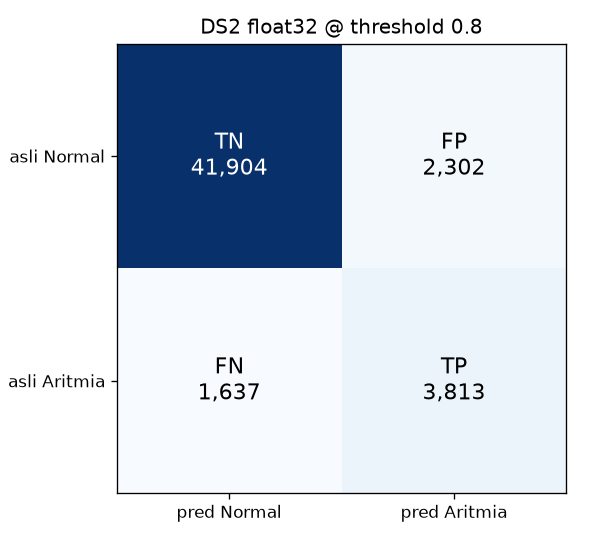
\includegraphics[width=\linewidth,keepaspectratio]{fase6_confusion_fp32.png}\\
    \small (a)
  \end{minipage}\hspace{0.05\linewidth}
  \begin{minipage}{0.4\linewidth}
    \centering
    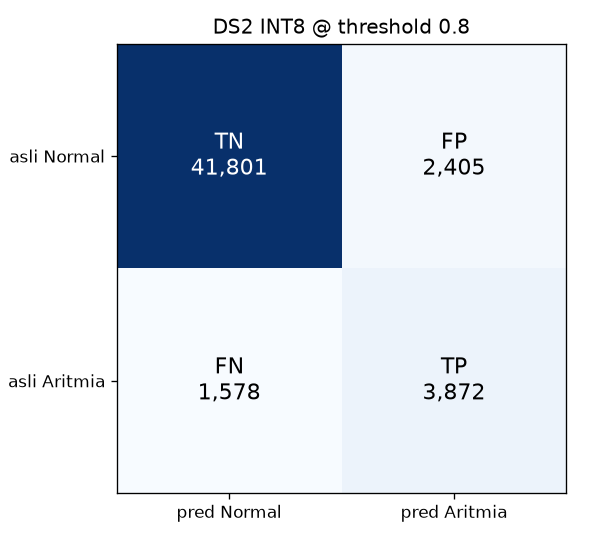
\includegraphics[width=\linewidth,keepaspectratio]{fase7_confusion_int8.png}\\
    \small (b)
  \end{minipage}
  \caption{\textit{Confusion matrix} DS2 pada \textit{threshold} 0,80, (a) model \textit{float32} dan (b) model INT8}
  \label{fig:cm-ds2}
\end{figure}

Pada Gambar~\ref{fig:cm-ds2}, baris adalah label sebenarnya dan kolom adalah prediksi. Model INT8 pada panel (b) menemukan 3.872 detak Aritmia, 59 lebih banyak daripada model \textit{float32} pada panel (a), dengan tambahan 103 FP dari 2.302 menjadi 2.405. Hasil kuantisasi ini bergantung pada varian \textit{deploy} yang dipakai. AveragePooling1D sempat dicoba sebagai pengganti, tetapi menurunkan \textit{recall} DS2 model versi lama dari 0,655 menjadi 0,528 karena operasi \textit{pooling} mewarisi skala kuantisasi masukannya.
% sumber: gambar laporan/buku-pa/gambar/fase6_confusion_fp32.png (TN 41.904, FP 2.302, FN 1.637, TP 3.813) dan fase7_confusion_int8.png (TN 41.801, FP 2.405, FN 1.578, TP 3.872), keduanya dibuka dan dibaca; 3.872 - 3.813 = 59; 2.405 - 2.302 = 103
% sumber: model/CLAUDE.md jebakan "Op pooling mewarisi skala kuantisasi input" (recall DS2 0,655 -> 0,528, skala input diwarisi)

\subsubsection{Kesetaraan dan Kinerja di Perangkat}

Butir ini bertujuan memastikan model INT8 memenuhi batas waktu dan memori di ESP32-S3. Kesetaraan keluarannya dengan PC sudah dibahas pada Subbab~\ref{subsec:hasil-tujuan1}, dan seluruh kasus uji di papan lulus, yaitu 16 kasus pada 18 September 2026 dan 29 kasus pada 13 Oktober 2026 setelah uji perangkat dan uji integrasi ditambahkan. Latensi diukur pada 18 September 2026 atas tujuh detak acuan pada CPU 240 MHz dengan \textit{kernel} referensi TensorFlow Lite Micro tanpa ESP-NN, sedangkan RAM dan Flash diambil dari laporan \textit{build} PlatformIO, seperti ditunjukkan pada Tabel~\ref{tab:sumber-daya}.
% sumber: firmware/test/test_inference/test_inference.cpp test_latensi_dan_memori (rata-rata us_terpakai atas GOLDEN_RR_FIRST sampai GOLDEN_N_BEAT = 7 detak, arena_used_bytes, ESP.getFreeHeap, getCpuFreqMHz); model/docs/firmware-walkthrough.md bagian 6 (240 MHz, kernel referensi tanpa ESP-NN); model/CLAUDE.md HW-1 dan HW-6 (pio test -e esp32-s3 16/16, angka diperbarui 18 Sep 2026); git log f6042b5 dan 07a5a07 (13 Okt 2026, board 29/29; angka latensi tidak dicatat ulang)

\begin{table}[!ht]
  \centering
  \caption{Pemakaian sumber daya model INT8 dan \textit{firmware} di ESP32-S3}
  \label{tab:sumber-daya}
  \setstretch{1.0}
  \setlength{\tabcolsep}{4pt}
  \renewcommand{\arraystretch}{1.15}
  \small
  \begin{tabular}{|>{\RaggedRight\arraybackslash}p{2.6cm}|>{\RaggedRight\arraybackslash}p{3.3cm}|>{\RaggedRight\arraybackslash}p{4.0cm}|>{\RaggedRight\arraybackslash}p{2.7cm}|}
    \hline
    \rowcolor{headgray}
    \textbf{Besaran} & \textbf{Nilai} & \textbf{Kondisi \textit{Build}} & \textbf{Target} \\
    \hline
    Ukuran model INT8 & 22,94 KB (23.488 byte) & Model INT8 format TensorFlow Lite, \textit{window} 256 & $<$ 25 KB \\
    \hline
    Latensi inferensi & 26,6 ms per detak & Uji perangkat, 240 MHz, \textit{kernel} referensi, \textit{window} 256 & Lebih kecil dari interval antardetak \\
    \hline
    \textit{Tensor arena} dan \textit{heap} bebas & 12.948 dari 24.576 byte, \textit{heap} bebas 312.396 byte & Uji perangkat, \textit{window} 256 & Muat di SRAM \\
    \hline
    RAM statis dan Flash & 74.284 byte (22,7\%) dan 430.569 byte (6,6\%) & \textit{Firmware} tanpa MQTT, dengan tabel \textit{replay} & Muat di memori \\
    \hline
    RAM statis dan Flash & 121.336 byte (37,0\%) dan 887.873 byte (13,5\%) & \textit{Firmware} dengan MQTT, kredensial WiFi terisi & Muat di memori \\
    \hline
  \end{tabular}
\end{table}
% sumber: model/docs/firmware-walkthrough.md bagian 6 (inferensi 26,6 ms, tensor arena 12.948 dari 24.576, model 22,94 KB, heap bebas 312.396, RAM 74.284 byte 22,7% dari 320 KB, Flash 430.569 byte 6,6% dari 6,25 MB); model/CLAUDE.md HW-1 (26,6 ms, 12.948 B, 312.396 B); model/docs/firmware-walkthrough.md bagian 6 dan model/docs/mqtt-walkthrough.md bagian 7 (build firmware utama dengan MQTT dan kredensial terisi: RAM 37,0% 121.336 B, Flash 13,5% 887.873 B; angka tanpa kredensial tidak dipakai; nilai lama 36,9% 121.008 B dan 881.861 B diperbarui 13 Okt 2026); firmware/src/klasifikasi.cpp ARENA_N = 24 * 1024; laporan/buku-pa/bab/bab3.tex tab:pengujian-model (target)

Berdasarkan Tabel~\ref{tab:sumber-daya}, latensi 26,6 ms setara paling banyak 13,3\% dari periode refraktori detektor 200 ms, yaitu interval antardetak terpendek, dan sekitar 4,4\% waktu CPU untuk inferensi saja pada laju \textit{replay} sekitar 1,6 detak per detik. \textit{Tensor arena} terpakai 52,7\% dari alokasinya. RAM statis naik dari 22,7\% menjadi 37,0\% dan Flash dari 6,6\% menjadi 13,5\% karena tumpukan WiFi dan klien MQTT ikut di-\textit{link}, dihitung terhadap RAM 320 KB dan partisi aplikasi 6,25 MB, dan angka ini hanya sah bila kredensial WiFi terisi (Subbab~\ref{subsec:validitas-pengukuran}). Seluruh besaran memenuhi target, sehingga model INT8 layak dijalankan secara \textit{on-device} tanpa \textit{cloud}, dengan keterbatasan bahwa latensi diukur tanpa WiFi aktif.
% sumber: tab:sumber-daya; firmware/include/ecg_preproc.h ECG_PT_REFRACTORY 72 sampel = 200 ms pada 360 Hz dan model/config.py PT_REFRACTORY_MS 200; 26,6 / 200 = 0,133; model/CLAUDE.md status HW-7 Replay dan model/docs/firmware-walkthrough.md §5c (11 detak per putaran 6,67 detik = 1,65 detak per detik), 26,6 x 11 / 6.670 = 0,044; 12.948 / 24.576 = 0,527; model/docs/firmware-walkthrough.md bagian 6 (320 KB, 6,25 MB)

\subsubsection{Konsumsi Daya}

Konsumsi daya per mode operasi belum terukur, sehingga target daya pada Tabel~\ref{tab:pengujian-model} belum dapat dinilai. Jalur pengukurannya telah tersedia di \textit{firmware}, yaitu enam tingkat beban bertahap pada Tabel~\ref{tab:tangga-daya} yang dapat dijalankan perangkat secara mandiri dari menu Ukur daya dengan catu baterai, pembacaan INA219 yang dirata-ratakan per jendela 10 detik, serta penyimpanan hasil per tingkat ke memori \textit{flash} beserta pemeriksaan keabsahannya. Jalur ini sudah diuji dari ujung ke ujung, yaitu keenam tingkat dapat dijalankan dengan sampel hilang nol pada setiap tingkat dan radio tersambung kembali pada tingkat 5, tetapi angka arusnya belum sah. Pada rangkaian saat ini papan masih dicatu langsung dari USB dan kedua pin masukan INA219 belum tersambung ke jalur arus, sehingga INA219 membaca tegangan bus sekitar 0 V dan arus yang tidak berasal dari beban. Pengukuran menunggu perakitan INA219 pada sisi baterai sesuai Subbab~\ref{subsec:perangkat-keras}. \PlaceholderData{arus, simpangan baku, tegangan, dan daya rata-rata per tingkat beban 0 sampai 5, selisih antartingkat, serta tingkat yang dinyatakan tidak sah bila ada}
% PLACEHOLDER-DATA daya: isi dari tangga mandiri (menu Ukur daya -> make pull-daya -> model/artifacts/metrics/daya/<YYYYmmdd-HHMM>-board-NNN.csv) atau dari laptop (model/scripts/measure_power.py -> model/artifacts/metrics/daya/<ts>.csv); 6 tingkat p0-p5, 6 jendela sah x 10 s per tingkat; kolom tabel: tingkat, I rata-rata (mA), sd, V, P (mW), sah; prosedur firmware/README.md bagian Ukur daya tanpa laptop dan model/docs/firmware-walkthrough.md §5d
% sumber: model/docs/firmware-walkthrough.md §5d "Kondisi jalur ukur saat ini" (13 Okt 2026, board dicatu USB laptop, bus 0-4 mV, shunt melompat 133-220 mV, VIN mengambang; jalur ukur diuji ujung ke ujung dengan --paksa, keenam mode terkonfirmasi, lewat = 0 di semua mode, radio tersambung kembali di p5); model/CLAUDE.md Pekerjaan terbuka "Konsumsi daya per mode operasi" (terhalang rangkaian); firmware/src/daya.cpp (tangga mandiri, hasil /daya/NNN.csv)

Pengukuran yang sah memerlukan beban yang identik pada setiap ulangan, sehingga seluruh tingkat memakai sinyal \textit{replay} acuan, dan perangkat mengalihkan sumber sensor ke \textit{replay} acuan selama pengukuran lalu mengembalikannya. Tingkat 5 memakai setelan radio tanpa mode tidur seperti pada pengujian \textit{pipeline}, karena setelan itu diperkirakan menambah arus sekitar 30~mA, dan memerlukan jaringan WiFi serta \textit{broker} yang terjangkau agar mewakili operasi normal.
% sumber: model/docs/firmware-walkthrough.md §5c "Sumber sinyal replay" (beban kerja identik tiap ulangan) dan §5d (sumber wajib replay, p5 setSleep(false)); firmware/README.md bagian Ukur daya tanpa laptop (ADC dialihkan ke replay acuan lalu kembali, WiFi dan broker harus terjangkau); model/docs/mqtt-walkthrough.md §7c dan §10 (setSleep(false) sekitar +30 mA)

\subsection{Jalur \textit{Pipeline Edge-to-Cloud} Resilien (Tujuan 3)}
\label{subsec:hasil-tujuan3}

Subbab ini menjawab Tujuan 3 pada Subbab~\ref{sec:tujuan}, yaitu membangun \textit{pipeline edge-to-cloud} yang resilien dengan protokol MQTT dan bufer lokal untuk menjamin kontinuitas data saat koneksi terputus. Keberhasilannya dinilai pada enam target di Tabel~\ref{tab:pengujian-pipeline}, dengan latensi dinilai pada median dan p95 dilaporkan (Tabel~\ref{tab:parameter-eksperimen}). Seluruh pengukuran dilakukan pada 19 September 2026 dengan sumber sinyal \textit{replay} rekaman 208 (Subbab~\ref{sec:karakteristik-data}), karena sinyal yang deterministik membuat hasil antarulangan dapat dibandingkan dan jumlah detak yang dikirim dapat dihitung secara pasti. Yang diuji karena itu adalah jalur dari pemrosesan di perangkat sampai \textit{dashboard}, bukan kualitas sinyal tubuh. Hasilnya dipaparkan dalam lima butir, yaitu gerbang kualitas, \textit{streaming} normal, putus koneksi, latensi, dan \textit{dashboard}.
% sumber: laporan/buku-pa/bab/bab1.tex Tujuan butir 3; laporan/buku-pa/bab/bab3.tex tab:pengujian-pipeline (enam aspek); bab4.tex tab:parameter-eksperimen baris f (latensi dinilai pada median, p95 dilaporkan) dan tab:lingkup-progres (pipeline MQTT dengan sinyal replay); model/docs/mqtt-walkthrough.md (19 September 2026); git log 6fc426c (2026-09-19)

\subsubsection{Gerbang Kalibrasi dan Kualitas Sinyal}

Butir ini bertujuan memastikan hanya detak dari sinyal layak yang masuk ke antrean dan dikirim ke \textit{cloud}. Rancangan pada Subbab~\ref{subsec:pipeline-edge-cloud}, dengan alur penilaian pada Gambar~\ref{fig:alir-firmware}, memuat dua gerbang, yaitu fase kalibrasi yang baru berakhir setelah elektroda stabil 10 menit, interval R-R berada pada 300--1500~ms dengan $|\Delta \mathrm{RR}| \leq 200$~ms selama 30 detik, dan ayunan tersaring mencapai 60 \textit{count}, lalu gerbang ayunan yang menilai setiap detak dari ayunannya saja. Seluruh uji pada subbab ini melewati syarat stabilisasi dan syarat R-R. Potongan 6,67 detik dari rekaman 208 yang diputar ulang bersifat aritmik dengan selisih R-R antardetak hingga $-$0,364 dan $+$0,478 detik sehingga kriteria R-R tidak akan terpenuhi, padahal kriteria itu dirancang untuk subjek sehat yang duduk diam. Gerbang masuk karena itu dilewati selama \textit{replay} aktif dan perangkat mengumumkan hal tersebut melalui serial, sedangkan stabilisasi ikut dilewati karena \textit{replay} tidak memakai elektroda. Pada pengujian ini pelewatan dinyalakan bersama \textit{replay}, sedangkan pada \textit{firmware} akhir pelewatan itu melekat pada sumber \textit{replay} dan berhenti begitu sumber kembali ke sensor (Subbab~\ref{subsec:pipeline-edge-cloud}), sehingga tidak dapat terbawa ke pemantauan sinyal tubuh.
% sumber: firmware/src/gerbang.cpp gerbang_nilai_fase() baris 227-249 (kalibrasi ke baik butuh stabil, rr_tenang, ayun_ok; sesudahnya fase = ayun_ok ? baik : buruk), baris 239-243 dan 523-527 (lewati_kalibrasi, replay) dan STABIL_MS 10 menit, RR_TENANG_MS 30 s, RR 0,300-1,500 s, DRR_MAKS 0,200 s, AMBANG_AYUN 60; model/docs/mqtt-walkthrough.md §3.1 dan §3.1b (dRR rekaman 208 terukur -0,364 s dan +0,478 s, kriteria RR gerbang masuk, toggle y menyalakan lewati_kalibrasi, pesan GERBANG DILEWATI (bench)); firmware/src/gerbang.cpp gerbang_nilai_fase() (firmware akhir: bypass melekat pada akuisisi_replay(), pesan GERBANG DILEWATI (replay)); model/docs/akuisisi-walkthrough.md §2; laporan/buku-pa/bab/bab3.tex subsec:pipeline-edge-cloud (alur gerbang pada fig:alir-firmware); potongan replay 6,67 detik: bab4.tex sec:karakteristik-data (golden_ref.h GOLDEN_N 2400, 2400 / 360 = 6,67 detik)

Yang benar-benar diuji karena itu hanya gerbang ayunan, dan pengujiannya mencakup dua arah. Sinyal \textit{replay} berayun sekitar 2.700 \textit{count}, lolos dengan nol detak ditahan, dan melewati gerbang ayunan lewat jalur kode yang sama dengan sinyal tubuh. Pada pengujian awal tanpa elektroda dengan gerbang ayunan saja, 19 detak terdeteksi, tujuh di antaranya diklasifikasi Aritmia, dan seluruhnya ditahan sehingga tidak satu pun terkirim ke \textit{broker}. Setelah fase kalibrasi ditambahkan, detak karangan tanpa elektroda berayun sekitar 27 \textit{count} dengan R-R 0,208 detik dan gagal pada kedua kriteria menurut catatan pengembangan, tetapi keluaran serialnya tidak disimpan. Batas pemisah antara elektroda lepas dan sinyal tubuh yang lemah belum diuji, karena ayunan \textit{replay} jauh di atas ambang 60 \textit{count} sedangkan keadaan tanpa elektroda berada di bawahnya. Gerbang ayunan karena itu terbukti bekerja pada kedua arah, sedangkan stabilisasi dan kriteria R-R tidak diuji dengan sinyal tubuh karena pengujian \textit{pipeline} memakai sinyal \textit{replay}.
% sumber: model/docs/mqtt-walkthrough.md bagian "Jalur data, terukur" (tanpa elektroda: beat 19 (7 aritmia, 19 ditahan) terkirim 0; replay: ditahan 0, terkirim 100%), §4.3 (ayunan replay sekitar 2700 counts, satu jalur kode tanpa cabang dummy) dan §10 (apakah AMBANG_AYUN 60 memisahkan elektroda lepas dari sinyal tubuh lemah belum teruji, replay terlalu jauh di atas ambang, gerbang kalibrasi penuh tertahan HW-5); model/CLAUDE.md HW-6 dan git show 33d9a80 (beat karangan tanpa elektroda gagal di dua gerbang, ayun 27 < 60 dan RR 0,208 s < 0,300 s, tertulis di pesan commit dan catatan, tidak ada berkas log keluaran serial); laporan/buku-pa/bab/bab4.tex tab:lingkup-progres (gerbang kalibrasi dengan sinyal tubuh ditunda)

\subsubsection{\textit{Streaming} Normal}

Butir ini bertujuan memastikan detak yang lolos gerbang sampai di ThingsBoard secara utuh dan tepat waktu pada jaringan yang tidak sengaja diganggu. Perangkat terhubung melalui WiFi lokal ke ThingsBoard di komputer pengembangan (Subbab~\ref{sec:tempat-ujicoba}), dan skrip pengukur \textit{pipeline} di komputer mengukur selama 180 detik sebanyak dua ulangan. Skrip membaca pencacah paket pada \textit{firmware} untuk PDSR dan membaca REST API ThingsBoard sekitar tiap 100~ms untuk latensi. PDSR dihitung per paket, bukan per detak, karena satu paket dapat memuat sampai 50 detak. Hasil keenam target ditunjukkan pada Tabel~\ref{tab:target-pipeline}.
% sumber: model/docs/mqtt-walkthrough.md §7c (dashboard/ukur_pipeline.py 180, replay ON, tanpa elektroda, dua ulangan); dashboard/ukur_pipeline.py (pencacah firmware lewat serial, polling REST dengan time.sleep(0.1)); firmware/include/ecg_mqtt.h (PDSR per paket, ECG_MQTT_BATCH_N 50); laporan/buku-pa/bab/bab4.tex sec:tempat-ujicoba

\begin{table}[!ht]
  \centering
  \caption{Hasil pengukuran enam target pengujian \textit{pipeline} pada dua ulangan dengan sumber sinyal \textit{replay}}
  \label{tab:target-pipeline}
  \setstretch{1.0}
  \setlength{\tabcolsep}{3pt}
  \renewcommand{\arraystretch}{1.15}
  \small
  \begin{tabular}{|>{\RaggedRight\arraybackslash}p{2.15cm}|>{\RaggedRight\arraybackslash}p{1.9cm}|>{\RaggedRight\arraybackslash}p{2.4cm}|>{\RaggedRight\arraybackslash}p{2.2cm}|>{\RaggedRight\arraybackslash}p{1.85cm}|>{\RaggedRight\arraybackslash}p{1.9cm}|}
    \hline
    \rowcolor{headgray}
    \textbf{Aspek} & \textbf{Metrik} & \textbf{Target} & \textbf{Ulangan 1} & \textbf{Ulangan 2} & \textbf{Status} \\
    \hline
    Keberhasilan pengiriman & PDSR & $\geq$ 95\% & 100,0\% (292 dari 292) & 99,2\% (253 dari 255) & Terpenuhi \\
    \hline
    Latensi \textit{end-to-end} & Median & $\leq$ 2 detik & 939~ms & 1.108~ms & Terpenuhi \\
    \hline
    Latensi \textit{end-to-end} & p95 & Dilaporkan, acuan $\leq$ 2 detik & 1.404~ms & 3.304~ms & Tidak stabil \\
    \hline
    Pemenuhan bufer lokal & Entri \textit{ring buffer} & Tidak \textit{overflow} dalam $\pm$27.000 & 27.000 terpasang, perilaku antrean penuh lulus uji unit & Konfigurasi sama & Terpenuhi \\
    \hline
    Integritas saat putus koneksi & Data hilang & Tanpa kehilangan & 0 (uji putus koneksi) & Tidak diulang & Terpenuhi \\
    \hline
    Pemulihan bufer & Durasi \textit{flush} & $\leq$ 60 detik & $\leq$ 24,6 detik (uji yang sama) & Tidak diulang & Terpenuhi \\
    \hline
    Deduplikasi \textit{cloud} & \textit{Timestamp} ganda & Duplikat QoS 1 dikenali dan diabaikan & 0 & Sama & Terpenuhi \\
    \hline
  \end{tabular}
\end{table}
% sumber: model/docs/mqtt-walkthrough.md §7c (Run 1 dan Run 2: PDSR 100,0% (292/292) dan 99,2% (253/255); median 939 dan 1.108 ms; p95 1.404 dan 3.304 ms; bufer lokal 27.000 terpasang; integritas hilang 0; pemulihan sekitar 24 dtk (43 beat), idem; deduplikasi 0 ts duplikat, idem; kolom idem pada baris ring, integritas, dan pemulihan merujuk satu skenario yang dicatat sekali pada konfigurasi awal sehingga ditulis Tidak diulang atau Konfigurasi sama, lihat git show 2857364 dan 33d9a80); 24,6 detik = 82,8 - 58,2 dari bagian "Uji resiliensi" (pembacaan status pertama sesudah tersambung kembali yang menunjukkan backlog 0); target dedup: bab3.tex Deduplikasi di ThingsBoard Rule Engine (ts_kv ditimpa, duplikat diabaikan); dan §7 (backlog 27.000 beat di PSRAM, 1.054 KB, 40 B per entri); model/CLAUDE.md HW-6 (6 dari 6 target terukur, 2 ulangan); target dari laporan/buku-pa/bab/bab3.tex tab:pengujian-pipeline dan bab4.tex tab:parameter-eksperimen baris f (latensi dinilai pada median, p95 dilaporkan); 253 / 255 = 0,9922

Berdasarkan Tabel~\ref{tab:target-pipeline}, PDSR dan median latensi memenuhi target pada kedua ulangan, sedangkan p95 tidak stabil dan dibahas pada butir d. Baris integritas dan pemulihan bersumber dari satu skenario putus koneksi (butir c), sedangkan baris bufer lokal menunjukkan kapasitas yang terpasang beserta perilaku antrean penuh yang diverifikasi pada uji unit. PDSR mencapai 100,0\% dan 99,2\%, di atas target 95\%. Pada ulangan kedua, dua dari 255 paket tidak tercatat menerima PUBACK. \textit{Firmware} hanya mengizinkan satu paket beredar, sehingga sekurang-kurangnya satu paket melewati batas 5 detik tanpa PUBACK lalu dikirim ulang dari antrean, dan detaknya tidak hilang karena baru dihapus setelah PUBACK. Penyebab pastinya tidak diperiksa, tetapi ulangan yang sama juga memiliki ekor latensi lebih panjang (butir d).
% sumber: laporan/buku-pa/bab/bab3.tex tab:pengujian-pipeline (PDSR >= 95%); firmware/src/ecg_mqtt.cpp ecg_mqtt_layani() baris 406-424 (menunggu_ack lalu return, satu PUBLISH beredar saja; PUBACK timeout 5000 ms memicu putus dan kirim ulang dari antrean) dan kirim_batch() (paket_kirim++ saat tulis, paket_ack++ saat PUBACK); model/docs/mqtt-walkthrough.md §7c (p95 3.304 ms pada Run 2, porsi paket lambat 24/255 = 9,4%); penyebab dua paket tidak dicatat di sumber manapun

Nol \textit{timestamp} ganda tidak berarti paket ganda tidak pernah tiba. Pengiriman ulang QoS 1 dapat mengirim detak yang sama dua kali, tetapi ThingsBoard menimpa baris yang \textit{timestamp}-nya sama. Mekanisme ini diuji dengan skrip uji asap (\textit{smoke test}) yang menerbitkan ulang sebuah \textit{timestamp} dengan nilai berbeda dan mendapati enam baris tanpa duplikat dengan nilai lama tertimpa. Baris integritas dan pemulihan bersumber dari satu skenario putus koneksi yang tidak diulang, sehingga kolom Ulangan 2 pada baris itu diisi Tidak diulang, dan cakupannya diuraikan pada butir c.
% sumber: dashboard/smoke_test.py (assert len(rows) == 6, len(by_ts) == 6, by_ts[base] == 999.0 setelah publikasi ulang ts identik); model/docs/mqtt-walkthrough.md §3.3 (uji dedup smoke_test tetap lulus); laporan/buku-pa/bab/bab3.tex Deduplikasi di ThingsBoard Rule Engine (upsert ts_kv); model/docs/mqtt-walkthrough.md §7c (0 ts duplikat); skenario putus koneksi satu kali: butir c subbab ini

Pada uji jalur data dan uji putus koneksi, pencacah sampel ADC yang hilang di perangkat tetap 0, sedangkan rancangan awal yang menunggu PUBACK di dalam \textit{loop} sempat menghilangkan 4.493 sampel (Tabel~\ref{tab:perubahan-rancangan}).
% sumber: model/docs/mqtt-walkthrough.md bagian "Jalur data, terukur" (baris "sampel hilang selama semua uji" bernilai 0, diukur di board 19 September 2026 bersama uji resiliensi docker pause) dan §7b bug 1 (4.493 sampel hilang, menjadi 146, hasil akhir 0 setelah bug 2); git show 2857364 (sampel hilang 0 pada pengukuran 171 baris / 103,2 detik); bab4.tex tab:perubahan-rancangan baris Transmisi (4.493); sumber hanya menulis "semua uji" tanpa merinci apakah pencacah dibaca pada uji pause secara terpisah

\subsubsection{Putus Koneksi dan Pemulihan}

Butir ini bertujuan memastikan tidak ada detak yang hilang ketika koneksi ke \textit{broker} terputus dan \textit{backlog} terkuras habis setelah koneksi pulih. Putusnya koneksi ditiru dengan membekukan \textit{container} ThingsBoard selama 24 detik saat \textit{replay} berjalan, lalu melanjutkannya kembali. Pembekuan dipilih karena \textit{container} yang beku tidak menjawab CONNECT sama sekali sehingga batas waktu \textit{connect} dan CONNACK ikut diuji, berbeda dengan \textit{container} yang dihentikan dan menjawab dengan pemutusan seketika. Skenario ini berbeda dari rencana pada Tabel~\ref{tab:pengujian-pipeline} yang menyebut pemutusan WiFi, dan sekaligus menguji deteksi koneksi \textit{half-open} lewat batas PUBACK 5 detik. Perubahan \textit{backlog} yang dicetak perangkat lewat serial ditunjukkan pada Gambar~\ref{fig:4-bufer}.
% sumber: model/docs/mqtt-walkthrough.md bagian "Uji resiliensi" (docker pause 24 detik, alasan pause dipilih dibanding stop, baris status) dan §4.4 (kolom status terkirim, backlog, hilang, gagal); laporan/buku-pa/bab/bab3.tex tab:pengujian-pipeline baris Integritas data saat putus koneksi (skenario putus WiFi paksa); firmware/src/ecg_mqtt.cpp baris 408 (PUBACK timeout 5000 ms memicu putus dan kirim ulang)

% PLACEHOLDER-GAMBAR fig:4-bufer  (plot data, skrip belum ada, tanya user dulu)
% Jenis      : plot data garis, landscape
% Pesan      : backlog naik selama broker beku lalu terkuras habis tanpa detak hilang
% Elemen     : sumbu x "Waktu (detik)" dan sumbu y "Backlog (detak)"; satu garis backlog; dua penanda vertikal "Broker dibekukan" pada 32,3 detik dan "Broker dilanjutkan" pada 56,1 detik; empat titik terukur pada 30,2 detik (1 detak), 54,0 detik (33), 58,2 detik (43), dan 82,8 detik (0); empat titik ditandai penanda dan dihubungkan garis putus-putus karena nilai antar-titik tidak diukur
% Alur baca  : kiri ke kanan, backlog hampir 0, naik selama broker beku sampai 43 detak, lalu terbaca 0 pada 82,8 detik, paling lama 24,6 detik sesudah perangkat tersambung kembali
% Teks       : label persis "Waktu (detik)", "Backlog (detak)", "Broker dibekukan", "Broker dilanjutkan"
% Bahan repo : model/docs/mqtt-walkthrough.md bagian "Uji resiliensi" (empat baris status bertanda waktu 30,2 s sampai 82,8 s). Titiknya sedikit, jadi untuk kurva yang halus uji perlu diulang dengan baris status 's' dicatat tiap detik. Skrip plot belum ada, tanyakan user dulu
% Ukuran     : width=\linewidth,keepaspectratio
\begin{figure}[!ht]
  \centering
  \PlaceholderGambar{Plot data}{jumlah detak pada bufer selama \textit{broker} dibekukan lalu dilanjutkan}
  \caption{Jumlah detak pada bufer selama \textit{broker} dibekukan 24 detik dan dikuras setelah dilanjutkan}
  \label{fig:4-bufer}
\end{figure}

Gambar~\ref{fig:4-bufer} memperlihatkan \textit{backlog} 1 detak pada 30,2 detik, sebelum \textit{broker} dibekukan pada 32,3 detik. Selama \textit{broker} beku, \textit{backlog} naik menjadi 33 detak pada 54,0 detik dan 43 detak pada 58,2 detik, saat perangkat tersambung kembali sekitar 2 detik setelah \textit{broker} dilanjutkan pada 56,1 detik. \textit{Backlog} terbaca 0 pada 82,8 detik, yaitu pembacaan status pertama sesudah tersambung kembali, sehingga pengurasan selesai paling lama 24,6 detik sementara detak baru tetap datang. Detak hilang tetap 0 dan hanya satu paket gagal tercatat, yang wajar karena \textit{broker} memang dibekukan. Pada deret waktu di ThingsBoard, jeda antar-\textit{timestamp} terbesar hanya 911~ms walaupun \textit{broker} beku 24 detik, karena detak yang tertahan dikirim dengan \textit{timestamp} waktu kejadian dan bukan waktu kirim, sehingga lubang pada grafik terisi oleh \textit{backlog}.
% sumber: model/docs/mqtt-walkthrough.md bagian "Uji resiliensi" ([30,2s] backlog 1; [32,3s] docker pause; [54,0s] backlog 33 gagal 1; [56,1s] docker unpause; [58,2s] tersambung, backlog 43 beat; [82,8s] backlog 0 hilang 0 gagal 1); 82,8 - 58,2 = 24,6 detik dan 56,1 - 32,3 = 23,8 detik; "gagal berhenti di 1, satu-satunya yang sah, saat broker memang dibekukan" (§7b bug 3); jeda maksimum 911 ms untuk outage 24 detik, backlog mengisi lubang dengan ts asli (bagian "Uji resiliensi" dan "Jalur data, terukur": 171 baris / 103,2 detik, 0 ts duplikat, jeda antar-ts 433-911 ms); firmware/src/klasifikasi.cpp publikasi() (ts dari r_abs, bukan waktu kirim)

Hasil ini memenuhi target tanpa kehilangan data dan pengurasan di bawah 60 detik. Cakupan skenarionya perlu dicatat. Putus koneksi ditiru dengan membekukan \textit{broker} dan bukan memutus WiFi. Skenario dicatat satu kali pada tahap awal pengembangan, ketika antrean berkapasitas 64 detak dan batas paket hanya 8 sampai 16 detak, sedangkan konfigurasi akhir berkapasitas 27.000 detak di PSRAM dengan paket 50 detak. Skenario itu tidak diulang pada konfigurasi akhir, sehingga jalur penulisan paket besar, yang pada konfigurasi awal sempat memotong paket 16 detak, tidak tercatat pernah diuji pada pengurasan di perangkat. Gangguan 24 detik hanya mengisi 43 dari 27.000 entri atau sekitar 0,16\%, sehingga kapasitas untuk $\pm$4--7 jam belum pernah diisi. Perilaku saat antrean penuh hanya diuji pada uji unit di komputer, dan waktu pengurasan untuk \textit{backlog} yang jauh lebih panjang belum diukur. Target integritas dan pemulihan karena itu terpenuhi pada skenario yang diuji, yaitu satu gangguan pendek terhadap \textit{broker}.
% sumber: model/docs/mqtt-walkthrough.md §7b bug 3 (paket 16 beat sekitar 4,8 KB terpotong karena sock.write() tidak habis, ECG_MQTT_BATCH_N 16 menjadi 8) dan git show 2857364 (pesan commit: payload besar 16 beat tidak habis ditulis, paket MQTT terpotong), git show 94dc0a0 (ring backlog 64 beat) dan 33d9a80 (ring 64 menjadi 27.000 beat di PSRAM, batch 16 menjadi 50, 27.000 x 40 B = 1,08 MB), git log -S"backlog 43 beat" (log resiliensi masuk di 2857364, sebelum 33d9a80); model/docs/mqtt-walkthrough.md §7c (pemulihan "~24 dtk (43 beat)", kolom Run 2 "idem"); 43 / 27.000 = 0,0016; firmware/test/test_mqtt/test_mqtt.cpp test_antre_penuh_buang_tertua (pio test -e native -f test_mqtt, 6 kasus lulus); firmware/src/ecg_mqtt.cpp ecg_mqtt_layani() (satu PUBLISH beredar saja)

\subsubsection{Latensi \textit{End-to-End}}

Butir ini bertujuan menilai apakah latensi dari terjadinya detak sampai tersedia di ThingsBoard memenuhi target 2 detik, dan menelusuri sumbernya. Latensi dihitung sebagai waktu komputer melihat baris telemetri di REST API dikurangi \textit{timestamp} baris itu, yaitu waktu kejadian R-\textit{peak}, dengan selisih jam perangkat dan komputer dikoreksi melalui epoch\_ms pada baris status. Alat ukur melaporkan batas bawah dan batas atas yang berselisih sebesar biaya \textit{polling} sekitar 100~ms, dan catatan hasil tidak menyebut batas yang dikutip sehingga angka dibaca dengan ketelitian sekitar 100~ms. Pada Tabel~\ref{tab:target-pipeline}, median 939 dan 1.108~ms memenuhi target, sedangkan p95 sebesar 1.404 dan 3.304~ms hanya memenuhi pada ulangan pertama.
% sumber: dashboard/ukur_pipeline.py (docstring dan kode: latensi = waktu laptop melihat ts baru dikurangi ts perangkat, ts_koreksi = ts - offset, offset dari epoch_ms, batas bawah memakai waktu sebelum REST dan batas atas sesudahnya, bias polling sekitar 100 ms, vonis memakai statistics.median(lo) <= 2000); model/docs/mqtt-walkthrough.md §7c (median 939 dan 1.108 ms, p95 1.404 dan 3.304 ms, minimum 429 dan 527 ms; batas yang dikutip tidak disebut)

Pengukuran awal memberi median 1.907~ms karena basis waktu perangkat semula berasal dari fungsi beresolusi satu detik (Subbab~\ref{subsec:validitas-pengukuran}), dan dekomposisi awal yang memakai angka itu keliru menyimpulkan bahwa sisa sekitar 1 detik milik \textit{broker}. Sesudah sumber waktu diganti dengan gettimeofday() dan selisih jam dikoreksi, median menjadi 939 sampai 1.108~ms, dan \textit{probe} yang menerbitkan 60 pesan berurutan ke \textit{broker} lewat antarmuka \textit{loopback} di komputer yang sama, tanpa melewati WiFi, mengukur waktu proses \textit{broker} 1,1~ms pada median dengan maksimum 3,5~ms dan tidak ada pesan di atas 1 detik. Dekomposisi yang berlaku ditunjukkan pada Tabel~\ref{tab:dekomposisi-latensi}.
% sumber: git show 33d9a80 (median 1.907 ms, sisa sekitar 1.033 ms milik broker) dan 6fc426c (koreksi: gettimeofday, latensi minimum 1.286 menjadi 429 ms, median 1.907 menjadi 939 ms); model/docs/mqtt-walkthrough.md §7b bug 6 dan §7c "KOREKSI" (probe 60 detik: minimum 0,4 ms, median 1,1 ms, p95 2,5 ms, maksimum 3,5 ms, > 1000 ms: 0 dari 60); dashboard/probe_rtt.py (socket.create_connection(("127.0.0.1", 1883)) yaitu antarmuka loopback tanpa WiFi, N 60 bawaan, satu PUBLISH QoS 1 per iterasi dan RTT sampai PUBACK); model/CLAUDE.md jebakan "time() beresolusi 1 detik" dan "Menyalahkan komponen jauh sebelum mengukurnya"

\begin{table}[!ht]
  \centering
  \caption{Dekomposisi latensi \textit{end-to-end} berdasarkan lokasi penundaan}
  \label{tab:dekomposisi-latensi}
  \setstretch{1.0}
  \setlength{\tabcolsep}{4pt}
  \renewcommand{\arraystretch}{1.15}
  \small
  \begin{tabular}{|>{\RaggedRight\arraybackslash}p{3.5cm}|>{\centering\arraybackslash}p{1.9cm}|>{\centering\arraybackslash}p{1.6cm}|>{\RaggedRight\arraybackslash}p{5.0cm}|}
    \hline
    \rowcolor{headgray}
    \textbf{Komponen} & \textbf{Nilai (ms)} & \textbf{Porsi} & \textbf{Keterangan} \\
    \hline
    Sisi perangkat, dari R-\textit{peak} sampai detak masuk antrean pengiriman & 869 & 87\% & Rerata dicacah \textit{firmware}, 869--887 pada 7 pengukuran, maksimum 1.353. Kadens deteksi 1 detik dan 356~ms sesudah R \\
    \hline
    Jaringan dan \textit{cloud}, dari antrean sampai terbaca di REST & $\approx$ 130 & 13\% & Selisih terhadap total, memuat pengiriman, WiFi, \textit{broker}, \textit{rule engine}, penyimpanan, dan bias \textit{polling} \\
    \hline
    Di dalamnya, \textit{broker} (RTT PUBACK) & 1,1 & $<$ 1\% & Median 60 pesan, diukur langsung dari komputer ke \textit{broker} \\
    \hline
    Total & $\approx$ 1.000 & 100\% & Dibulatkan dari median 939 dan 1.108, sehingga porsi bergeser antara 78\% dan 93\% menurut ulangan \\
    \hline
  \end{tabular}
\end{table}
% sumber: model/docs/mqtt-walkthrough.md §7c "Latensi dipecah" (tunda alat 887 / 880 / 879 / 878 / 876 / 870 / 869 ms, maks 1.353 ms; sisi alat 869 ms; jaringan + cloud sekitar 130 ms; latensi median sekitar 1.000 ms; broker 1,1 ms); firmware/src/klasifikasi.cpp publikasi() baris 285-287 (tunda = millis() - t.ms dihitung saat detak dimasukkan ke antrean, bukan saat paket ditulis ke soket seperti tertulis di catatan pengembangan, tunda_jml / tunda_n = rerata, tunda_maks); 869 / (869 + 130) = 0,870 sehingga 87%, catatan pengembangan menulis 89% yang tidak dapat direproduksi dari kedua komponen; 130 / 999 = 0,130; 128 / 360 = 0,356 detik; porsi per ulangan: 869 / 939 = 0,925 (93%) dan 869 / 1.108 = 0,784 (78%)

Berdasarkan Tabel~\ref{tab:dekomposisi-latensi}, sekitar 87\% latensi berasal dari sisi perangkat bila total dibulatkan menjadi 1.000~ms, atau 93\% pada ulangan pertama dan 78\% pada ulangan kedua, dan bagian itu bersifat arsitektural. Deteksi dijalankan tiap 1 detik atas \textit{ring} 4 detik dan detak baru boleh keluar 128 sampel atau 356~ms sesudah puncak R, sehingga penundaan berada di antara 356 dan 1.356~ms, dengan rerata sekitar 856~ms bila setiap detak menunggu siklus deteksi setengah detik, sejalan dengan 869~ms yang terukur. Jaringan dan \textit{cloud} menyumbang sisanya, sekitar 130~ms pada total yang dibulatkan dan sudah termasuk bias \textit{polling}, sedangkan \textit{broker} sendiri 1,1~ms. Menurunkan kadens deteksi menjadi 0,5 detik diperkirakan memangkas sekitar 250~ms dari rerata, tetapi menggandakan frekuensi deteksi yang bebannya belum diukur ulang, sedangkan median sudah memenuhi target, sehingga perubahan itu tidak dilakukan dalam penelitian ini.
% sumber: tab:dekomposisi-latensi; perkiraan kadens 0,5 detik (perhitungan): rerata tunggu siklus 0,5 detik menjadi 0,25 detik sehingga rerata 356 + 500 = 856 ms menjadi 356 + 250 = 606 ms, selisih 250 ms; beban deteksi pada kadens 1 detik: tab:beban-komputasi; model/docs/mqtt-walkthrough.md §7c (ecg_live.h menjalankan deteksi tiap ECG_LIVE_TIAP = 1 detik atas ring 4 detik, beat keluar setelah ECG_WIN_POST = 128 sampel = 356 ms, batas bawah teoretis 356-1.356 ms, minimum terukur 429 ms); firmware/include/ecg_live.h (ECG_LIVE_TIAP, ECG_LIVE_RING 4 * ECG_FS); 356 + 1.000 = 1.356 dan 356 + 500 = 856 (perhitungan, siklus deteksi seragam terhadap waktu detak); git show 33d9a80 (menurunkan kadens menyentuh modul tervalidasi golden Python-C, gate point, tidak diubah)

Ekor sebaran adalah kelemahan terukur pada butir ini. RTT PUBACK yang dicatat perangkat berkelompok di sekitar 1,2, 2,0, dan 4,2 detik, yang menyerupai pola penggandaan \textit{retransmission timeout} TCP saat segmen yang hilang di WiFi dikirim ulang. Penyebab lain sudah dikesampingkan, yaitu \textit{broker} menjawab dalam 1,1~ms, soket kosong ketika PUBACK melewati batas waktu sehingga aliran baca tidak bergeser, dan kuat sinyal $-$50 dBm bukan sinyal lemah. Dugaan yang tersisa adalah kontensi kanal pada jaringan yang tidak terisolasi (Subbab~\ref{sec:tempat-ujicoba}), yang belum diukur langsung.
% sumber: model/docs/mqtt-walkthrough.md §7c "Ekor p95" (RTT PUBACK berkelompok 1,2 / 2,0 / 4,2 detik, backoff RTO TCP 1-2-4, sock.available() = 0 byte saat timeout, RSSI -50 dBm, kontensi kanal WiFi) dan model/CLAUDE.md jebakan "Menyalahkan komponen jauh sebelum mengukurnya"; firmware/src/ecg_mqtt.cpp (komentar setSleep: RTT 1.236 / 2.037 / 4.235 ms); laporan/buku-pa/bab/bab4.tex sec:tempat-ujicoba (WiFi tidak terisolasi)

Dua penanganan diterapkan, yaitu setNoDelay(true) agar algoritma Nagle tidak menahan paket kecil dan WiFi.setSleep(false) agar radio tidak tidur dan menjatuhkan paket masuk. Porsi paket ber-RTT di atas 1 detik turun dari 11,1\% (23 dari 207 paket) menjadi 8,1\% dan 5,1\% pada kedua langkah itu, lalu terukur 1,0\% (3 dari 292) dan 9,4\% (24 dari 255) pada dua ulangan di Tabel~\ref{tab:target-pipeline}, sehingga berayun antara 1 dan 9\%. Penurunan menjadi 8,1\% dan 5,1\% tidak dapat dipisahkan dari ayunan antarulangan tersebut, dan yang berubah antarulangan adalah kondisi kanal, bukan kode. Sisa ekor tidak dikejar karena satu-satunya langkah pada \textit{firmware} yang tersisa, yaitu \textit{pipelining} QoS 1, mengubah implementasi QoS 1 yang sederhana dan terbukti demi 1 sampai 9\% paket pada jaringan di tempat uji, sedangkan median dan PDSR sudah memenuhi target. Setelan setSleep(false) menambah arus yang diperkirakan sekitar 30~mA dan belum diukur, sehingga pengukuran daya WiFi harus memakainya (Subbab~\ref{subsec:hasil-tujuan2}), dan p95 yang bersih memerlukan titik akses yang tidak padat dengan lebih banyak ulangan.
% sumber: model/docs/mqtt-walkthrough.md §7c (tabel perubahan dan paket lambat: awal 23/207 = 11,1%, setNoDelay 18/222 = 8,1%, setSleep(false) 11/217 = 5,1%, dua run terakhir 3/292 = 1,0% dan 24/255 = 9,4%) dan §7b bug 5 (Nagle berpasangan dengan delayed-ACK, RTT berulang sekitar 1.250 ms); firmware/src/ecg_mqtt.cpp baris 322-330 (WiFi.setSleep(false)) dan 392-399 (sock.setNoDelay(true)); penyebut 292 dan 255 sama dengan jumlah paket Run 1 dan Run 2 pada tab:target-pipeline
% sumber: model/docs/mqtt-walkthrough.md §7c "Keputusan: tidak dikejar lebih jauh" (pipelining QoS-1 menambah pembukuan pid dan beat dan aturan geser ring setelah ack tertua, kejadian 1-dari-20 di jaringan uji, median dan PDSR lulus, bab3 menyebut target indikatif dan pengujian fungsional bukan klinis; kalau butuh p95 bersih ukur di AP tidak padat dan laporkan n run), setSleep(false) sekitar +30 mA (biaya daya, perkiraan) tanpa pengukuran HW-7 mode WiFi; porsi paket lambat 23/207, 18/222, 11/217, 3/292, 24/255 dari tabel §7c; firmware/src/ecg_mqtt.cpp komentar setSleep; laporan/buku-pa/bab/bab3.tex Rencana Pengujian (bukan klinis, target indikatif)

\subsubsection{\textit{Dashboard}}

Butir ini bertujuan memastikan data yang tiba di ThingsBoard dapat dibaca pada \textit{dashboard} yang dikonfigurasi tanpa pemrograman \textit{frontend}, dengan tujuh \textit{widget} bawaan ThingsBoard CE 4.2.1.1 sesuai Tabel~\ref{tab:widget-thingsboard} yang dirakit melalui skrip penyiapan \textit{dashboard} lewat REST API agar dapat diulang, dan tampilannya ditunjukkan pada Gambar~\ref{fig:4-dashboard}.
% sumber: dashboard/README.md bagian Dashboard (tujuh widget bawaan, dibangun dengan provision_dashboard.py lewat REST agar bisa diulang); dashboard/docker-compose.yml (thingsboard/tb-postgres:4.2.1.1); laporan/buku-pa/bab/bab3.tex tab:widget-thingsboard

\begin{figure}[!ht]
  \centering
  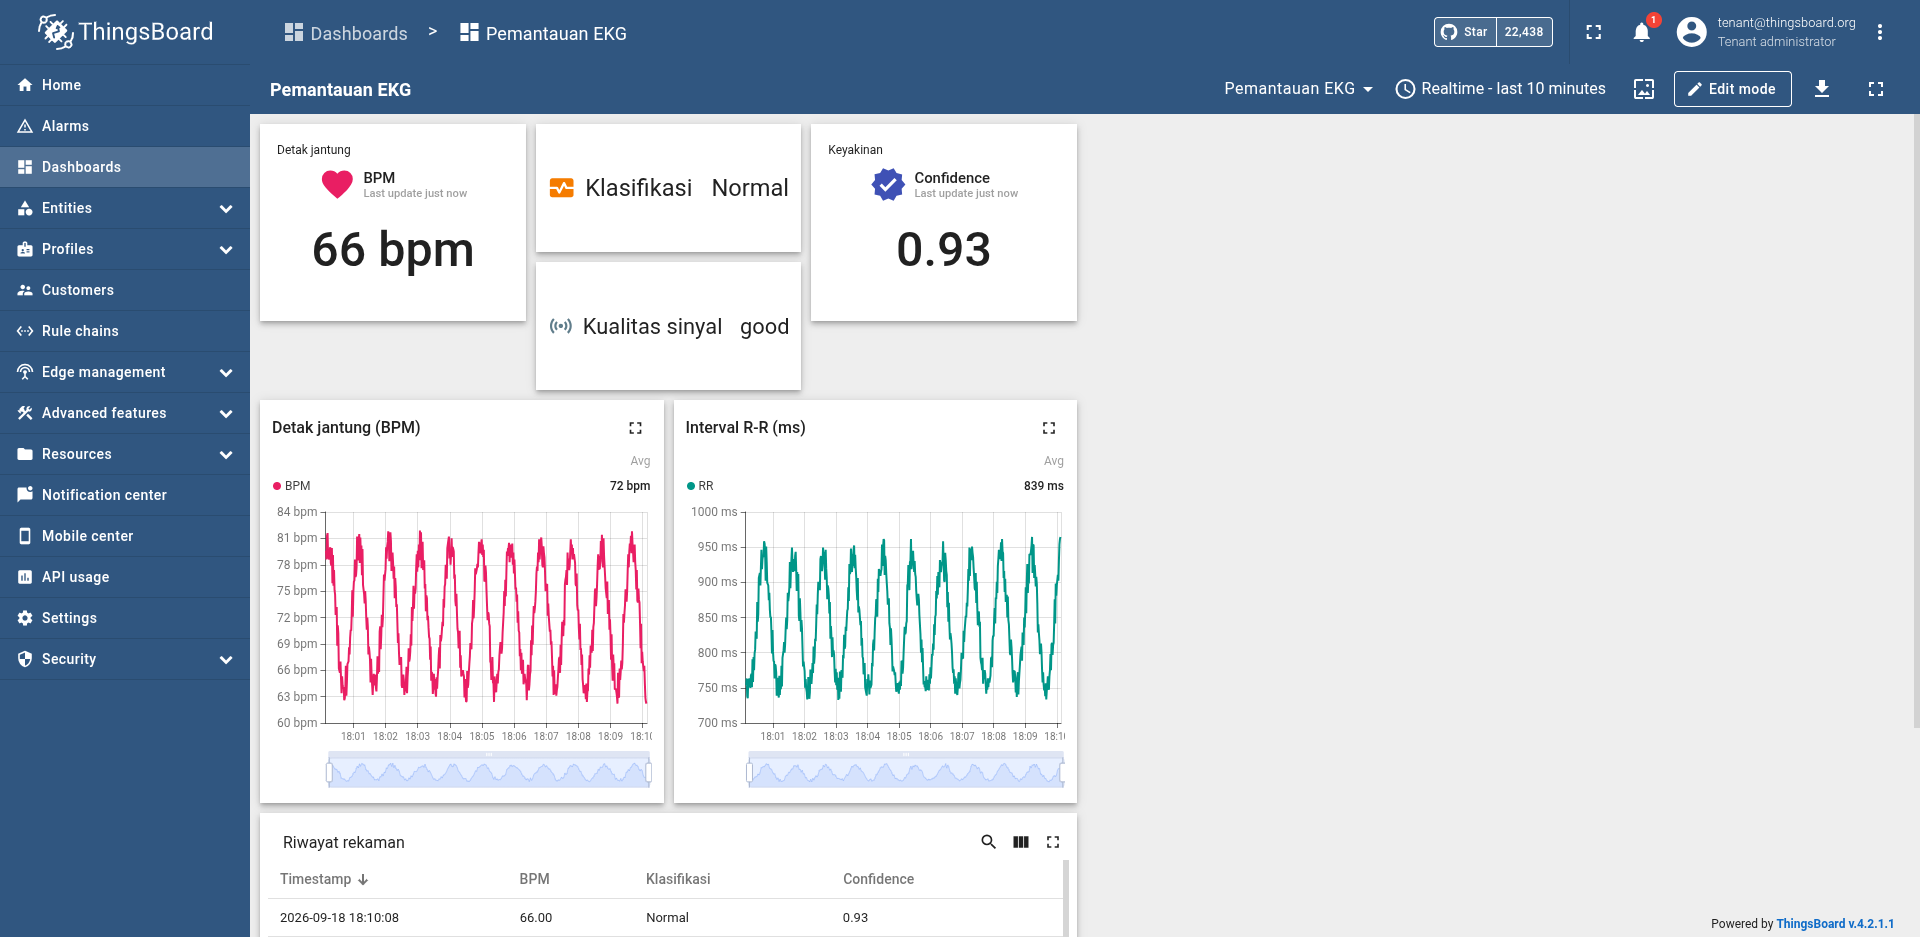
\includegraphics[width=\linewidth,keepaspectratio]{dashboard_preview.png}
  \caption{Tampilan \textit{dashboard} Pemantauan EKG pada ThingsBoard dengan telemetri uji tanggal 18 September 2026}
  \label{fig:4-dashboard}
\end{figure}

Gambar~\ref{fig:4-dashboard} diambil pada 18 September 2026, sebelum klien MQTT perangkat selesai, dan nilai \textit{confidence} 0,93 sama dengan konstanta \textit{payload} pada skrip uji asap. Data yang tampak karena itu adalah telemetri uji dan bukan keluaran perangkat, sehingga gambar hanya menunjukkan tata letak \textit{widget}, yaitu kartu BPM, klasifikasi, \textit{confidence}, dan kualitas sinyal di bagian atas, dua grafik tren BPM dan interval R-R di tengah, serta tabel riwayat rekaman di bagian bawah. Tangkapan layar dengan telemetri perangkat belum diambil, aturan alarm belum dipasang, dan ecg\_snippet belum memiliki \textit{widget} walaupun datanya sudah tiba.
% KONFIRMASI PENULIS: ambil ulang tangkapan layar dengan telemetri replay perangkat
% sumber: gambar laporan/buku-pa/gambar/dashboard_preview.png (dibuka dan dibaca: kartu BPM 66 bpm, Klasifikasi Normal, Kualitas sinyal good, Confidence 0.93, grafik Detak jantung (BPM) rerata 72 bpm sumbu 60-84 bpm, grafik Interval R-R (ms) rerata 839 ms sumbu 700-1000 ms, tabel Riwayat rekaman 2026-09-18 18:10:08 BPM 66.00 Normal 0.93; tata letak kartu di atas, dua grafik di tengah, tabel di bawah); dashboard/provision_dashboard.py (WIDGETS)
% sumber: dashboard/preview.png (berkas 18 Sep 2026 20:09, identik dengan laporan/buku-pa/gambar/dashboard_preview.png), git log b906903 (2026-09-18 19:59, dashboard dibuat) dan 94dc0a0 (2026-09-19 20:01, klien MQTT perangkat pertama); dashboard/smoke_test.py record() (confidence 0.93, signal_quality good, label_str Normal); laporan/buku-pa/bab/bab3.tex Antarmuka Monitoring (aturan alarm belum dipasang); model/docs/mqtt-walkthrough.md §10 (widget ecg_snippet belum digambar); sumber data tampilan diinferensikan dari kesamaan nilai, bukan dari log

Dengan demikian keenam target terukur dengan sinyal \textit{replay}, tiga di antaranya pada dua ulangan, dan seluruhnya terpenuhi. PDSR dan median latensi memenuhi target pada kedua ulangan, p95 tidak stabil karena kondisi kanal, dan putusnya koneksi selama 24 detik tidak menghilangkan satu detak pun. Gerbang masuk dengan sinyal tubuh, skenario putus koneksi pada kapasitas akhir bufer, dan latensi pada jaringan yang tidak padat berada di luar cakupan pengujian ini dan dicatat sebagai keterbatasan.
% sumber: tab:target-pipeline; butir a sampai d pada subbab ini; tiga target pada dua ulangan adalah PDSR, latensi, dan deduplikasi (model/docs/mqtt-walkthrough.md §7c, kolom Run 1 dan Run 2), sedangkan bufer lokal, integritas, dan pemulihan bersumber dari konfigurasi dan skenario yang tidak diulang

\section{Analisis Hasil Eksperimen}
\label{sec:analisis}

Subbab ini menilai hasil pada Subbab~\ref{sec:hasil-eksperimen} terhadap ketiga tujuan pada Subbab~\ref{sec:tujuan}. Status Tercapai diberikan bila seluruh target pada rencana pengujian terukur dan terpenuhi, sedangkan Sebagian Tercapai diberikan bila ada target yang belum terukur. Tujuan 3 berstatus Tercapai. Tujuan 1 berstatus Sebagian Tercapai karena akuisisi sinyal tubuh belum diuji melalui pengujian rekaman resmi, walaupun seluruh target jalur komputasi terpenuhi, sedangkan Tujuan 2 berstatus Sebagian Tercapai karena konsumsi daya per mode operasi belum diukur, walaupun seluruh target model dan kinerja di perangkat terpenuhi. Penilaian dirangkum pada Tabel~\ref{tab:ketercapaian} dan alasannya diuraikan per tujuan pada subbab berikutnya.
% PLACEHOLDER-DATA status-tujuan1: status Tujuan 1 dinilai ulang setelah tab:kualitas-rekaman terisi dari pengujian rekaman resmi (Tercapai bila kriteria kualitas terpenuhi)

\begin{table}[!ht]
  \centering
  \caption{Ketercapaian tujuan penelitian}
  \label{tab:ketercapaian}
  \setstretch{1.0}
  \setlength{\tabcolsep}{3pt}
  \renewcommand{\arraystretch}{1.15}
  \small
  \begin{tabular}{|>{\RaggedRight\arraybackslash}p{2.4cm}|>{\RaggedRight\arraybackslash}p{3.1cm}|>{\RaggedRight\arraybackslash}p{3.3cm}|>{\RaggedRight\arraybackslash}p{1.6cm}|>{\RaggedRight\arraybackslash}p{2.3cm}|}
    \hline
    \rowcolor{headgray}
    \textbf{Tujuan} & \textbf{Target} & \textbf{Hasil} & \textbf{Status} & \textbf{Justifikasi} \\
    \hline
    Tujuan 1\newline Preprocessing \textit{real-time} &
    Setara dengan Python dalam toleransi data acuan, tanpa sampel hilang, dan sinyal tubuh memenuhi kriteria kualitas &
    Seluruh tahap uji data acuan lulus, beban 3,0\% anggaran, sampel hilang 0, sinyal tubuh \PlaceholderData{jumlah rekaman Berhasil dari jumlah sesi} &
    Sebagian Tercapai &
    Jalur komputasi terbukti setara, akuisisi sinyal tubuh menunggu pengujian resmi \\
    % PLACEHOLDER-DATA ketercapaian-tujuan1: kolom Hasil dan Status diisi ulang dari tab:kualitas-rekaman setelah pengujian rekaman resmi
    % sumber: bab4 tab:uji-kesetaraan-tahap, tab:beban-komputasi, tab:kualitas-rekaman; target dari bab3 tab:pengujian-model dan bab4 tab:parameter-eksperimen baris d dan e
    \hline
    Tujuan 2\newline Model INT8 \textit{on-device} &
    $|\Delta \textit{recall}| < 0{,}02$, model $<$ 25~KB, latensi di bawah interval antardetak, muat di SRAM, daya per mode &
    $\Delta$\textit{recall} $+$0,0108, 22,94~KB, 26,6~ms per detak, \textit{arena} 12.948 byte, F1 INT8 0,6604, daya belum diukur &
    Sebagian Tercapai &
    Target model dan perangkat terpenuhi, konsumsi daya belum diukur \\
    % sumber: bab4 tab:delta-int8, tab:sumber-daya, subsec:hasil-tujuan2 butir Konsumsi Daya; target dari bab3 tab:pengujian-model
    \hline
    Tujuan 3\newline \textit{Pipeline} MQTT resilien &
    PDSR $\geq$ 95\%, median latensi $\leq$ 2 detik, tanpa \textit{overflow} dan data hilang, \textit{flush} $\leq$ 60 detik, duplikat dikenali &
    PDSR 100,0\% dan 99,2\%, median 939 dan 1.108~ms, duplikat 0, hilang 0 dan \textit{flush} $\leq$ 24,6 detik pada uji putus koneksi &
    Tercapai &
    Seluruh target terpenuhi, p95 di luar target tidak stabil \\
    % sumber: bab4 tab:target-pipeline (seluruh baris Terpenuhi; hilang 0 dan flush <= 24,6 detik dari satu uji putus koneksi, p95 tidak stabil dan bukan target); target dari bab3 tab:pengujian-pipeline dan bab4 tab:parameter-eksperimen baris f
    \hline
  \end{tabular}
\end{table}

Berdasarkan Tabel~\ref{tab:ketercapaian}, seluruh target yang bergantung pada komputasi dan pengiriman data terpenuhi. Target yang belum dapat dinilai adalah kualitas sinyal tubuh pada Tujuan 1, yang menunggu pengujian rekaman resmi, dan konsumsi daya per mode operasi pada Tujuan 2.

\subsection{Ketercapaian Tujuan 1}
\label{subsec:analisis-tujuan1}

Jalur komputasi preprocessing terbukti setara dengan Python dan berjalan secara \textit{real-time}. Seluruh tahap pada Tabel~\ref{tab:uji-kesetaraan-tahap} lulus, termasuk 11 R-\textit{peak} yang sama dengan Python dalam toleransi 1 sampel dan keputusan akhir yang identik pada tujuh detak acuan. Beban rata-rata hanya 82 $\mu$s per sampel atau 3,0\% anggaran, dan sampel hilang tetap 0 walaupun puncak beban sesaat mencapai 33,4~ms (Tabel~\ref{tab:beban-komputasi}). Kesetaraan ini dijamin oleh koefisien filter dan model yang dihasilkan otomatis dari Python lalu diuji tahap demi tahap, sedangkan ADC yang dibaca di ISR dan antrean 256 sampel menyerap \textit{burst} deteksi dan inferensi, sehingga syarat pada Tabel~\ref{tab:pengujian-model} terpenuhi.
% sumber: bab4 tab:uji-kesetaraan-tahap (11 puncak, toleransi 1 sampel, label identik 7 detak), tab:beban-komputasi (82 us, 3,0%, 33,4 ms, sampel hilang 0, antrean 256), sec:karakteristik-data butir penyelarasan (berkas ecg_preproc.h dan model_int8.h dihasilkan otomatis)

Kelayakan sinyal tubuh sebagai masukan jalur ini dinilai melalui pengujian rekaman resmi, yaitu \PlaceholderData{jumlah rekaman yang memenuhi kriteria kualitas pada Tabel~\ref{tab:kualitas-rekaman} dari jumlah sesi perekaman}. Segmentasi hasil detektor tidak merusak klasifikasi, dengan F1 0,6499 dibandingkan 0,6594 pada segmentasi anotasi (Tabel~\ref{tab:segmentasi-deteksi}). Catatannya, kesetaraan tahap demi tahap dibuktikan pada sinyal \textit{replay} sepanjang 6,67 detik tanpa kelas S, beban rata-rata diukur pada model \textit{window} 250, dan detektor menemukan kelas S dengan \textit{sensitivity} 0,6494 (Tabel~\ref{tab:sensitivity-detektor}). Tujuan 1 karena itu dinilai Sebagian Tercapai, karena jalur komputasi memenuhi seluruh targetnya sedangkan akuisisi sinyal tubuh belum diuji secara resmi.
% PLACEHOLDER-DATA analisis-tujuan1: kalimat pertama dan status akhir diisi ulang dari tab:kualitas-rekaman setelah pengujian rekaman resmi
% sumber: bab4 subsec:hasil-tujuan1 butir port C (rekaman 208, 6,67 detik, tanpa kelas S) dan butir alur hidup (window 250), tab:sensitivity-detektor (S 0,6494), tab:segmentasi-deteksi

\subsection{Ketercapaian Tujuan 2}
\label{subsec:analisis-tujuan2}

Model INT8 berjalan secara \textit{on-device} di ESP32-S3 dalam batas waktu dan memori yang ditargetkan. Kuantisasi hanya menggeser \textit{recall} sebesar $+$0,0108 dengan ukuran 22,94~KB, keduanya di bawah ambang rencana pengujian (Tabel~\ref{tab:delta-int8}), inferensi memakan 26,6~ms per detak atau paling banyak 13,3\% dari interval antardetak terpendek 200~ms, dan \textit{tensor arena} terpakai 12.948 dari 24.576 byte (Tabel~\ref{tab:sumber-daya}). Hasil ini bergantung pada varian \textit{deploy} berbasis DepthwiseConv1D, karena operasi MEAN pada TensorFlow Lite Micro salah hitung tanpa pesan kesalahan dan hanya terungkap oleh uji data acuan (Tabel~\ref{tab:perubahan-rancangan}).
% sumber: bab4 tab:delta-int8 (+0,0108, 22,94 KB), tab:sumber-daya dan paragraf sesudahnya (26,6 ms, 13,3% dari 200 ms, 12.948 dari 24.576 byte), tab:perubahan-rancangan baris Model deploy

Kualitas klasifikasi, yang tidak memiliki ambang angka, mencapai \textit{recall} 0,6996, F1 0,6594, dan AUC 0,9334 pada model \textit{float32} (Tabel~\ref{tab:hasil-ds2}) dengan median \textit{recall} per pasien 0,9167. Kelemahan terbesarnya adalah kelas S dengan \textit{recall} 0,4390, karena QRS-nya mirip Normal dan pembedanya terletak pada waktu kedatangan serta gelombang P, dan kelemahan ini terbawa ke data uji SVDB dan INCART dengan \textit{recall} S konfigurasi terkunci 0,2494 dan 0,1503 (Subbab~\ref{subsec:hasil-tujuan2}). Target daya belum dapat dinilai karena INA219 belum dirakit pada jalur catu baterai walaupun jalur pengukurannya di \textit{firmware} sudah siap, dan latensi diukur tanpa WiFi aktif. Tujuan 2 karena itu dinilai Sebagian Tercapai, karena target kuantisasi, ukuran, latensi, dan memori terpenuhi, sedangkan konsumsi daya belum diukur.
% sumber: bab4 tab:hasil-ds2 (0,6996, 0,6594, 0,9334), subsec:hasil-tujuan2 butir Evaluasi DS2 (median per pasien 0,9167, recall S 0,4390, alasan QRS mirip Normal), butir Ablasi (TEST-B 0,2494, TEST-C 0,1503), butir Konsumsi Daya (INA219 belum dirakit di sisi baterai), paragraf sesudah tab:sumber-daya (latensi tanpa WiFi aktif)

\subsection{Ketercapaian Tujuan 3}
\label{subsec:analisis-tujuan3}

\textit{Pipeline} MQTT dengan bufer lokal memenuhi target \textit{streaming} pada dua ulangan dengan sumber \textit{replay}, yaitu PDSR 100,0\% dan 99,2\% serta median latensi 939 dan 1.108~ms, sedangkan p95 tidak stabil. Pada satu uji putus koneksi tidak ada detak hilang dan pengurasan selesai paling lama 24,6 detik. \textit{Timestamp} ganda tidak ditemukan pada kedua ulangan (Tabel~\ref{tab:target-pipeline}). Kontinuitas pada uji putus koneksi berasal dari antrean yang baru melepas detak setelah PUBACK diterima dan dari \textit{timestamp} berisi waktu kejadian, sehingga jeda terbesar pada deret waktu hanya 911~ms selama \textit{broker} beku 24 detik. Median latensi dibatasi arsitektur deteksi dan bukan jaringan, karena sekitar 87\% latensi, atau 78\% sampai 93\% menurut ulangan, berasal dari sisi perangkat dan \textit{broker} hanya 1,1~ms (Tabel~\ref{tab:dekomposisi-latensi}).
% sumber: bab4 tab:target-pipeline (100,0% dan 99,2%, 939 dan 1.108 ms, p95 tidak stabil, hilang 0 dan flush <= 24,6 detik dari satu uji, ts ganda 0 pada dua ulangan), subsec:hasil-tujuan3 butir Streaming Normal (dihapus setelah PUBACK, ThingsBoard menimpa ts sama) dan butir Putus Koneksi (jeda 911 ms, beku 24 detik, antrean pada uji itu masih berkapasitas 64 detak), tab:dekomposisi-latensi (87%, rentang 78% sampai 93%, 1,1 ms)

Cakupan pengujiannya perlu dicatat. Seluruh pengukuran memakai sinyal \textit{replay} sekitar 1,6 detak per detik dengan hanya gerbang ayunan yang diuji, skenario putus koneksi dijalankan satu kali sebelum antrean dipindahkan ke PSRAM berkapasitas 27.000 entri dengan paket 50 detak, dan p95 berayun antara 1.404~ms dan 3.304~ms yang diduga akibat kontensi kanal WiFi. Karena seluruh target pada Tabel~\ref{tab:pengujian-pipeline} terpenuhi pada pengujian yang dilakukan, Tujuan 3 dinilai Tercapai, dengan cakupan tersebut dicatat sebagai keterbatasan.
% sumber: bab4 sec:karakteristik-data butir replay (sekitar 1,6 detak per detik), subsec:hasil-tujuan3 butir Gerbang (hanya gerbang ayunan), butir Putus Koneksi (satu kali, antrean 64 detak, konfigurasi akhir 27.000 entri dan paket 50 detak), tab:target-pipeline (p95 1.404 dan 3.304 ms), butir Latensi (dugaan kontensi kanal)

\subsection{Perbandingan dengan Penelitian Terkait}
\label{subsec:analisis-perbandingan}

Perbandingan dibatasi pada penelitian yang skema evaluasinya diuraikan pada Subbab~\ref{sec:penelitian-terkait}, yaitu Zambrano-de la Torre et al.~\cite{zambrano_2026} dan penelitian pendahulu~\cite{mulyawan_2026} yang memakai platform sensor dan \textit{dashboard} yang sama, dan protokolnya disandingkan pada Tabel~\ref{tab:perbandingan-protokol}.

\begin{table}[!ht]
  \centering
  \caption{Perbandingan protokol evaluasi dengan penelitian terkait}
  \label{tab:perbandingan-protokol}
  \setstretch{1.0}
  \setlength{\tabcolsep}{3pt}
  \renewcommand{\arraystretch}{1.15}
  \small
  \begin{tabular}{|>{\RaggedRight\arraybackslash}p{2.3cm}|>{\RaggedRight\arraybackslash}p{2.0cm}|>{\RaggedRight\arraybackslash}p{2.5cm}|>{\RaggedRight\arraybackslash}p{2.4cm}|>{\RaggedRight\arraybackslash}p{3.5cm}|}
    \hline
    \rowcolor{headgray}
    \textbf{Penelitian} & \textbf{Kelas} & \textbf{Pembagian Data} & \textbf{Lokasi Inferensi} & \textbf{Hasil yang Dilaporkan} \\
    \hline
    Zambrano-de la Torre et al.~\cite{zambrano_2026} &
    Tiga kelas, yaitu N, V, dan S &
    Per detak tanpa pemisahan antarpasien pada MIT-BIH &
    Arduino UNO 8-bit, 1D-CNN INT8 &
    \textit{Accuracy}, degradasi kuantisasi $<$ 0,7\%, model $<$ 22~KB, latensi sekitar 200~ms per detak \\
    % sumber: bab2 subsec:related-zambrano2026 dan tab:perbandingan-penelitian baris 11
    \hline
    Penelitian pendahulu~\cite{mulyawan_2026} &
    Atrial fibrilasi &
    Pengujian \textit{offline}, dilatih pada MIT-BIH &
    SVM di \textit{backend cloud}, ESP32 untuk akuisisi dan fitur R-R &
    \textit{Accuracy} tinggi pada pengujian \textit{offline} \\
    % sumber: bab2 subsec:related-mulyawan2026 dan tab:perbandingan-penelitian baris 12 (tanpa angka akurasi)
    \hline
    Penelitian ini &
    Biner, yaitu Normal dan Aritmia &
    \textit{Inter-patient} DS1/DS2, DS2 berisi 22 pasien &
    ESP32-S3, model \textit{hybrid} INT8 \textit{on-device} &
    INT8 pada DS2 \textit{recall} 0,7105, F1 0,6604, AUC 0,9344, \textit{accuracy} 0,9198, model 22,94~KB, latensi 26,6~ms per detak \\
    % sumber: bab4 tab:delta-int8 (INT8), tab:sumber-daya (26,6 ms), subsec:hasil-tujuan2 butir Evaluasi DS2 (22 pasien)
    \hline
  \end{tabular}
\end{table}

Berdasarkan Tabel~\ref{tab:perbandingan-protokol}, angka ketiga penelitian tidak dapat dibandingkan langsung karena kelas, pembagian data, dan metriknya berbeda. Pembagian per detak membuat detak dari pasien yang sama dapat muncul di himpunan latih dan uji, sedangkan DS2 berisi 22 pasien yang tidak pernah dilihat saat pelatihan (Subbab~\ref{subsec:evaluasi-metrik}). Latensi juga tidak dibandingkan karena Arduino UNO 8-bit dan ESP32-S3 berbeda kelas. Pada sisi metrik, 89,0\% detak DS2 berlabel Normal sehingga menebak Normal untuk seluruh detak sudah memberi \textit{accuracy} sekitar 0,89 (Subbab~\ref{sec:parameter-eksperimen}), dan \textit{accuracy} model ini, yaitu 0,9207 pada \textit{float32} dan 0,9198 pada INT8, hanya sekitar 3 poin di atasnya (Tabel~\ref{tab:delta-int8}). \textit{Accuracy} pada data setimpang ini belum menunjukkan kemampuan mendeteksi aritmia, sehingga hasil penelitian ini dilaporkan melalui \textit{recall}, F1, dan AUC.
% sumber: bab2 subsec:evaluasi-metrik (pembagian per detak optimistis, sekitar 89% Normal, akurasi sekitar 0,89), bab4 sec:parameter-eksperimen (89,0%, sekitar 0,89), subsec:hasil-tujuan2 butir Evaluasi DS2 (accuracy 0,9207 sekitar 3 poin di atas tebak Normal), tab:delta-int8 (0,9207 dan 0,9198)

Terhadap penelitian pendahulu yang mendeteksi atrial fibrilasi dengan SVM di sisi \textit{cloud}~\cite{mulyawan_2026}, penelitian ini melanjutkan dengan memindahkan klasifikasi per detak ke ESP32-S3 dan menambahkan bufer lokal yang menjaga data tetap utuh selama \textit{broker} tidak terjangkau (Tabel~\ref{tab:target-pipeline}). Protokol \textit{inter-patient} disadari membuat angka penelitian ini tampak lebih rendah daripada \textit{accuracy} pada pembagian per detak, dan angka DS2 pun berpotensi sedikit optimistis karena DS2 dipakai menilai ablasi \textit{window} dan \textit{jitter}. Penelitian ini karena itu tidak mengklaim \textit{accuracy} yang lebih tinggi, melainkan evaluasi yang lebih ketat terhadap pasien baru, inferensi di perangkat yang setara dengan Python, dan \textit{pipeline} yang tidak kehilangan data pada skenario putus koneksi yang diuji.
% sumber: bab2 subsec:related-mulyawan2026 (SVM di backend cloud, AFib); bab4 tab:sumber-daya (26,6 ms), tab:target-pipeline (data hilang 0), subsec:hasil-tujuan2 butir Evaluasi DS2 (DS2 menilai ablasi window dan jitter, berpotensi sedikit optimistis), tab:uji-kesetaraan-tahap

\subsection{Keterbatasan dan Status \textit{Proof of Concept}}
\label{subsec:analisis-keterbatasan}

Walaupun jalur komputasi, model INT8, dan \textit{pipeline} telah terukur di perangkat, sistem ini berstatus \textit{proof of concept} di lingkungan non-klinis dan bukan alat diagnosis (Subbab~\ref{sec:batasan-masalah}), dengan keterbatasan yang diuraikan pada butir berikut.
\begin{enumerate}
  \item Rekaman perangkat berasal dari \PlaceholderData{jumlah subjek} subjek sehat yang dianonimkan, sehingga variasi sinyal antarindividu belum terwakili.
  \item Rekaman sinyal tubuh yang memenuhi kriteria berjumlah \PlaceholderData{jumlah rekaman Berhasil dari jumlah sesi} (Tabel~\ref{tab:kualitas-rekaman}), sehingga variasi antarsesi baru terwakili secara terbatas.
  % PLACEHOLDER-DATA keterbatasan-rekaman: butir 1 dan 2 diisi dari data primer dan tab:kualitas-rekaman pengujian resmi; sesuaikan kalimatnya bila jumlah subjek atau sesi sudah memadai
  \item Konsumsi daya belum diukur, termasuk biaya daya radio WiFi yang tidak ditidurkan.
  \item Ekor latensi belum stabil, yaitu p95 1.404~ms dan 3.304~ms pada dua ulangan yang diduga akibat kontensi kanal WiFi.
  \item Model hanya biner dan tidak menamai jenis aritmia, sesuai Batasan Masalah.
  \item \textit{Recall} kelas S masih rendah, juga lintas basis data. \textit{Learning rate} $10^{-3}$ tetap dipakai demi kelas S karena $10^{-4}$ menurunkan \textit{recall} S DS2 dari 0,4473 menjadi 0,3126 walaupun AUC naik (Tabel~\ref{tab:ablasi}), dengan konsekuensi model akhir hasil satu \textit{epoch}.
  \item Angka DS2 berpotensi sedikit optimistis karena DS2 ikut menilai ablasi \textit{window} dan \textit{jitter}.
  \item Uji \textit{pipeline} memakai sinyal \textit{replay}, sehingga perilakunya pada sinyal tubuh dengan laju dan kualitas yang berubah-ubah belum diukur.
  \item Gerbang kualitas baru diuji pada gerbang ayunan, sedangkan stabilisasi elektroda, kriteria R-R, dan batas antara elektroda lepas dan sinyal lemah belum diuji.
  \item Uji putus koneksi dijalankan satu kali pada konfigurasi awal dan hanya mengisi 43 dari 27.000 entri atau sekitar 0,16\% kapasitas akhir.
\end{enumerate}
% sumber: bab4 sec:karakteristik-data butir data primer, tab:kualitas-rekaman, subsec:hasil-tujuan2 butir Konsumsi Daya dan subsec:hasil-tujuan3 butir Latensi (setSleep(false) menambah arus, belum diukur), tab:target-pipeline (p95), bab1 sec:batasan-masalah butir 1, tab:ablasi (0,4473 dan 0,3126) dan butir Ablasi (satu epoch), butir Evaluasi DS2 (DS2 ikut menilai ablasi window dan jitter, berpotensi sedikit optimistis), subsec:hasil-tujuan3 butir Gerbang dan Putus Koneksi (43 dari 27.000, 0,16%), subsec:hasil-tujuan1 butir Segmentasi (0,6661 menjadi 0,5656, window 250)

Sebagian besar keterbatasan tersebut berkaitan dengan cakupan uji, bukan dengan jalur komputasi, dan arah pengembangannya dirangkum sebagai saran pada Bab~\ref{chap:penutup}.
